%%%%%%%%%%%%%%
%% Run LaTeX on this file several times to get Table of Contents,
%% cross-references, and citations.

%% If you have font problems, you may edit the w-bookps.sty file
%% to customize the font names to match those on your system.

%% w-bksamp.tex. Current Version: Feb 16, 2012
%%%%%%%%%%%%%%%%%%%%%%%%%%%%%%%%%%%%%%%%%%%%%%%%%%%%%%%%%%%%%%%%
%
%  Sample file for
%  Wiley Book Style, Design No.: SD 001B, 7x10
%  Wiley Book Style, Design No.: SD 004B, 6x9
%
%
%  Prepared by Amy Hendrickson, TeXnology Inc.
%  http://www.texnology.com
%%%%%%%%%%%%%%%%%%%%%%%%%%%%%%%%%%%%%%%%%%%%%%%%%%%%%%%%%%%%%%%%

%%%%%%%%%%%%%
\documentclass{wileySev}

\usepackage{graphicx}

%%%%%%%
%% for times math: However, this package disables bold math (!)
%% \mathbf{x} will still work, but you will not have bold math
%% in section heads or chapter titles. If you don't use math
%% in those environments, mathptmx might be a good choice.

% \usepackage{mathptmx}

% For PostScript text
\usepackage{w-bookps}

%%%%%%%%%%%%%%%%%%%%%%%%%%%%%%%%%%%%%%%%%%%%%%%%%%%%%%%%%%%%%%%%
%% Other packages you might want to use:

% for chapter bibliography made with BibTeX
% \usepackage{chapterbib}

% for multiple indices
% \usepackage{multind}

% for answers to problems
% \usepackage{answers}

\usepackage[svgnames]{xcolor} % Required to specify font color
\usepackage[utf8]{inputenc}
\usepackage[portuguese]{babel}

\usepackage{indentfirst}
\usepackage{float}

\usepackage{listings} % Required for inserting code snippets
\usepackage[usenames,dvipsnames]{} % Required for specifying custom colors and referring to colors by name
%%%%%%%%%%%%%%%%%%%%%%%%%%%%%%
%% Change options here if you want:
%%
%% How many levels of section head would you like numbered?
%% 0= no section numbers, 1= section, 2= subsection, 3= subsubsection
%%==>>
\setcounter{secnumdepth}{3}

%% How many levels of section head would you like to appear in the
%% Table of Contents?
%% 0= chapter titles, 1= section titles, 2= subsection titles,
%% 3= subsubsection titles.
%%==>>
\setcounter{tocdepth}{2}

\newcommand{\VT}[1]{\ensuremath{{V_{T#1}}}}

%% use a box to expand the macro before we put it into the section head:

\newbox\sectsavebox
\setbox\sectsavebox=\hbox{\boldmath\VT{xyz}}

\newcommand*{\plogo}{\hspace*{-1cm}
\includegraphics[width=200px]{images/logo}} % Generic publisher logo

\setcounter{secnumdepth}{5}

%----------------------------------------------------------------------------------------
%	TITLE PAGE
%----------------------------------------------------------------------------------------

\newcommand*{\titleGP}{\begingroup % Create the command for including the title page in the document
\centering % Center all text
\vspace*{\baselineskip} % White space at the top of the page

\rule{\textwidth}{1.6pt}\vspace*{-\baselineskip}\vspace*{2pt} % Thick horizontal line
\rule{\textwidth}{0.4pt}\\[\baselineskip] % Thin horizontal line

{\normalsize Projeto Integrado}\\[0.2\baselineskip] {\LARGE BILL MATE \\[0.3\baselineskip]} {\large Engenharia de Aplicações 13/14}\\[0.2\baselineskip] % Title

\rule{\textwidth}{0.4pt}\vspace*{-\baselineskip}\vspace{3.2pt} % Thin horizontal line
\rule{\textwidth}{1.6pt}\\[\baselineskip] % Thick horizontal line

\scshape % Small caps
A partilha de despesas nunca foi tão fácil \\ % Tagline(s) or further description
[\baselineskip] % Tagline(s) or further description
{\itshape Universidade do Minho\par} % Editor affiliation

\vspace*{\baselineskip} % Whitespace between location/year and editors

\vfill % Whitespace between editor names and publisher logo

\plogo \\[\baselineskip] % Publisher logo
%\vspace*{2\baselineskip} % Whitespace
\vfill
Braga,  2013--2014\par % Location and year

\endgroup}

%----------------------------------------------------------------------------------------
%	SNIPPETS CONFIGURATIONS
%----------------------------------------------------------------------------------------



\definecolor{DarkGreen}{rgb}{0.0,0.4,0.0} % Comment color
\definecolor{highlight}{RGB}{255,251,204} % Code highlight color

\lstdefinestyle{Style1}{ % Define a style for your code snippet, multiple definitions can be made if, for example, you wish to insert multiple code snippets using different programming languages into one document
%language=Perl, % Detects keywords, comments, strings, functions, etc for the language specified
backgroundcolor=\color{highlight}, % Set the background color for the snippet - useful for highlighting
basicstyle=\footnotesize\ttfamily, % The default font size and style of the code
breakatwhitespace=false, % If true, only allows line breaks at white space
breaklines=true, % Automatic line breaking (prevents code from protruding outside the box)
captionpos=b, % Sets the caption position: b for bottom; t for top
commentstyle=\usefont{T1}{pcr}{m}{sl}\color{DarkGreen}, % Style of comments within the code - dark green courier font
deletekeywords={}, % If you want to delete any keywords from the current language separate them by commas
%escapeinside={\%}, % This allows you to escape to LaTeX using the character in the bracket
firstnumber=1, % Line numbers begin at line 1
frame=single, % Frame around the code box, value can be: none, leftline, topline, bottomline, lines, single, shadowbox
frameround=tttt, % Rounds the corners of the frame for the top left, top right, bottom left and bottom right positions
keywordstyle=\color{Blue}\bf, % Functions are bold and blue
morekeywords={}, % Add any functions no included by default here separated by commas
numbers=left, % Location of line numbers, can take the values of: none, left, right
numbersep=10pt, % Distance of line numbers from the code box
numberstyle=\tiny\color{Gray}, % Style used for line numbers
rulecolor=\color{black}, % Frame border color
showstringspaces=false, % Don't put marks in string spaces
showtabs=false, % Display tabs in the code as lines
stepnumber=5, % The step distance between line numbers, i.e. how often will lines be numbered
stringstyle=\color{Purple}, % Strings are purple
tabsize=2, % Number of spaces per tab in the code
}

% Create a command to cleanly insert a snippet with the style above anywhere in the document
\newcommand{\insertcode}[2]{\begin{itemize}\item[]\lstinputlisting[caption=#2,label=#1,style=Style1]{#1}\end{itemize}} % The first argument is the script location/filename and the second is a caption for the listing


%----------------------------------------------------------------------------------------
%	BLANK DOCUMENT
%----------------------------------------------------------------------------------------

\newcommand{\specialcell}[2][c]{%
  \begin{tabular}[#1]{@{}c@{}}#2\end{tabular}
  }


\newcommand*{\titleTH}{\begingroup
\raggedleft
\vspace*{\baselineskip}

{\Large Universidade do Minho}\\[0.167\textheight]
{\LARGE\bfseries Projeto Integrado}\\[\baselineskip]
{\Huge Bill Mate}\\[\baselineskip]
{\Large \textit{Engenharia de Aplicações 13/14}}\par

\vfill

\large{André Santos pg25329\\Pedro Leite pg25330\\Francisco Neves pg25334\\Ricardo Branco pg25339}\par

\vspace*{3\baselineskip}
\endgroup}

\begin{document}

\titleGP % This command includes the title page

\booktitle{BILLMATE}
\subtitle{Partilha de Despesas}

\authors{André Santos PG25329\\
		\affil{Universidade do Minho}
		Pedro Leite PG25330\\
		\affil{Universidade do Minho}
		Francisco Neves PG25334\\
		\affil{Universidade do Minho}
		Ricardo Branco PG25339\\
		\affil{Universidade do Minho}
}

\titlepage

\begin{resumo}

Os projetos devem ser realizados com base em ideias novas, e não se devem focar em reinventar a roda. Foi este objetivo que moveu o grupo, e que desde o inicio pensou em realizar algo diferente e que fizesse a diferença no dia-a-dia do público-alvo.

Desde cedo surgiram várias ideias, e todas elas tinham bastante potencial, porém, o grupo queria algo que fosse útil para uso próprio e para aquelas que nos rodeiam. Assim, idealizou-se uma aplicação que pudesse ser realizada em contexto académico mas que no final da sua implementação pudesse ficar online para todos utilizarem. Com isto, pensou-se sobre uma aplicação que ajudasse na divisão de despesas entre um grupo de pessoas.

Dito isto, iniciou-se uma pesquisa que permitiu concluir que já existem algumas com o mesmo objetivo, mas, constatou-se que todas elas tentam ser muito genéricas, perdendo alguma abstração aquando da sua integração com diferentes tipos de utilizadores, e no caso dos estudantes, o grupo verificou que as existentes não abordam conceitos como "pagamento da eletricidade", ou um simples "pagamento da internet".

Com base nesta investigação, focou-se o público-alvo para estudantes, e inseriram-se todos os conceitos importantes para uma gestão organizada das despesas dos mesmos. \\\\

\textbf{Área de aplicação:} Desenvolvimento de aplicação para suportar o processo da partilha de despesas entre estudantes. Implementação de infra-estrutura aplicacional, avaliação e desempenho e escalabilidade. \\\\

\textbf{Palavras-chave:} Tomcat, Grails, Spring, WebService, CentOS, LVS, DRBD, NFS, ISCSI, MPATH, REDIS.

\end{resumo}

\contentsinbrief
\tableofcontents
\listoffigures
\listoftables

%\begin{preface}
%Fazer um pequeno resumo do projeto.


\prefaceauthor{Pedro Leite}
\where{Braga, Portugal\\
Abril, 2014}
\mbox{}\\%Dou uma opinião


\prefaceauthor{André Santos}
\where{Braga, Portugal\\
Abril, 2014}
\mbox{}\\%André dá uma opinião


\prefaceauthor{Francisco Neves}
\where{Braga, Portugal\\
Abril, 2014}
\mbox{}\\%Francisco dá uma opinião


\prefaceauthor{Ricardo Branco}
\where{Braga, Portugal\\
Abril, 2014}
\mbox{}\\%Ricardo dá uma opinião

\end{preface}
\begin{acronyms}

\acro{DRBD}{Distributed Replicated Block Device}
\acro{HTML}{Hypertext Mark Language}
\acro{ICD}{Infraestrutura de Centros de Dados}
\acro{IDE}{Integrated Development Environment}
\acro{ISCSI}{Internet Small Computer System Interface}
\acro{LVS}{Linux Virtual Server}
\acro{MPATH}{Multipath}
\acro{NFS}{Network File System}
\acro{SO}{Sistema Operativo}
\acro{UCE}{Unidade Curricular de Especialização}
\acro{VM}{Virtual Machine}

\end{acronyms}
\begin{glossary}

\term{Term} Term description

\end{glossary}


\setcounter{page}{1}
\pagestyle{headings}

\chapter[Introdução]
{Introdu\c{c}\~ao}


O trabalho que se encontra documentado neste relatório é relativo ao Projeto Integrado enquadrado na UCE de Engenharia de Aplicações, sendo que o objetivo deste projeto é conseguir utilizar os conceitos abordados nos quatro módulos desta UCE para se conseguir construir uma plataforma que suporte a aplicação com alta disponibilidade e com segurança.

Com base neste objetivo, delineou-se o desenvolvimento de uma aplicação de despesas partilhadas entre estudantes. Esta ideia surge porque, a maioria dos jovens começa a ter mais necessidades de organização aquando da sua chegada à universidade, que é quando normalmente sai da casa dos pais, e precisa de começar a pagar as suas obrigações, sejam elas de eletricidade, de gás, entre outras. Com base nisto, é certo que por várias vezes, as dívidas caem em esquecimento, e muitas são as histórias de terem ficado sem eletricidade, sem gás ou sem internet por falta de pagamento.

O nome \emph{BillMate} é uma concatenação de \emph{Bill} com \emph{Mate}, que significa exatamente aquilo que esta aplicação faz, que é a partilha de despesas entre colegas. Esta é uma excelente ferramenta para os estudantes, porque é feita por estudantes, que sabem exatamente as suas necessidades. É certo que não há melhor cliente do que o próprio cliente, uma vez que conhece todas as suas necessidades. Além disso, a facilidade de confrontar o público-alvo com esta aplicação, irá permitir que esta seja mais cómoda para o utilizador final.

O trabalho que se documenta neste relatório, descreve todo o processo de criação de uma aplicação que suporta a divisão de despesas de estudantes, ajudando a fazer a divisão entre os diversos grupos em que se encontra, para que este saiba em qualquer momento, as despesas que já estão pagas, as datas limite de pagamento, as próximas despesas, as pessoas que já pagaram, entre vários outros componentes que se referirão nos capítulos posteriores.

Os capítulos encontram-se organizados estrategicamente, apresentando-se Inicialmente uma motivação para a realização deste projeto, de modo que o utilizador final perceba quais os problemas que esta aplicação vem resolver. Esta conclusão do utilizador final terá mais ênfase quando confrontado com os casos de estudo que aparecerão posteriormente. Após estes, serão verificados os requisitos e o planeamento tomado em consideração. Com isto, entrar-se-à em detalhes mais técnicos, onde será descrita toda a infraestrutura que suportará a aplicação, passando pela modelação, interface e implementação da codificação do sistema.
Terminando todo este processo serão apresentados os resultados de desempenho da aplicação na infraestrutura desenvolvida.

\chapter[Motivação]
{Motiva\c{c}\~ao}

Todas as pessoas necessitam de organizar os seus débitos e os seus ativos, porém, por lapso ou por falta de tempo, nem sempre se lembram de todas as suas obrigações. No caso dos estudantes universitários, isto ainda é um fator mais agravante, porque estes começam a sentir esta necessidade quando vão para a universidade, porque a maior parte destes, saem da casa dos pais nesta altura, o que implica que iniciam novas responsabilidades que até este momento não tinham.

Muitas são as histórias de falta de eletricidade, falta de gás, ou até mesmo de falta de internet por atraso no pagamento. Esta aplicação tende a responder a estas necessidades. Estes problemas são contornados devido aos alertas e notificações que são enviados ao utilizador para que este não se esqueça das suas obrigações.

A grande vantagem desta aplicação, deve-se ao facto de ser elaborada por estudantes, e destinar-se a estudantes, pois, quem está a fazer a aplicação sabe as necessidades para este contexto. Não há melhor cliente do que quem elabora o produto, porque sabe todos os seus requisitos. O feedback demonstrado pelo público-alvo tem sido bastante positivo, demonstrando bastante interesse pelo resultado final desta aplicação.

Esta aplicação é bastante ambiciosa, porque a ambição do grupo também é bastante relevante, uma vez que no final deste trabalho, pretende-se que esta aplicação não fique "apenas no papel", e que saia do contexto académico, ficando online e disponível para todas as pessoas.

\chapter[Casos de estudo]
{Casos de estudo}

De seguida serão apresentados alguns casos de estudo, nos quais se verifica o comportamento em algumas das situações que o grupo identificou. Apesar de apenas se apresentarem três casos de estudo, é fácil de compreender, que muitos outros cenários se enquandram nos apresentados.

\section{Caso 1 - Habitação}

O Pedro, o André, o Francisco e o Ricardo são estudantes universitários e vivem todos na mesma habitação. Para uma melhor organização das despesas utilizam uma aplicação para fazer esta gestão. O Pedro criou uma habitação e associou os 4 amigos à mesma. Nesta habitação criou uma despesa regular de eletricidade para o dia 23 de Julho, que se repete mensalmente. No dia 23 de Julho, o Pedro recebe o aviso da despesa regular e cria a despesa da eletricidade associando a imagem da fatura à despesa.

Os restantes elementos da casa recebem o aviso indicando o valor monetário que devem ao Pedro, e efetuam o pagamento. Todos fazem o pagamento, e após o Pedro confirmar o pagamento de todos os elementos, a despesa fica resolvida. Por uma questão de organização, o Pedro decide adicionar ainda o comprovativo do recibo para que todos possam consultar e fazer download dos documentos.
\section{Caso 2 - Boleias}

O André, o Francisco e o Ricardo vivem na mesma área de residência e partilham o mesmo carro para irem para a universidade. Além deles, ainda costumam dar boleia ao Pedro, mas o Pedro mora bastante mais perto da universidade, pelo que ficou decidido que o Pedro iria pagar apenas 10\% da despesa.

O André, que é o condutor, criou um grupo para boleias e associou-os aos 4 a esse grupo. De seguida colocou o valor da despesa total, e definiu as percentagens de pagamento. Para o Pedro apenas colocou 10\% e para os restantes dividiu de forma equitativa (30\%).

Todos fizeram o pagamento e confirmaram o mesmo. O André após receber o dinheiro também confirmou a receção do mesmo. Uma vez que tanto o credor como o devedor confirmaram, então a dívida é confirmada e encerrada.

No final, a despesa da boleia é confirmada e encerrada, uma vez que já todos pagaram o pagameto.
\section{Caso 3 - Jantar}

O Pedro, o André, o Francisco e o Ricardo foram jantar a seguir às aulas, mas quem pagou toda a despesa foi o Pedro. Com o objetivo de controlar quem já pagou e quem ainda falta pagar, o Pedro criou um grupo e associou os amigos à mesma, e dividiu a despesa pelos seus amigos.

Os seus amigos recebem a notificação, procedem ao pagamento e confirmam o pagamento. De seguida o Pedro confirma que recebeu a quantia monetária. Mas, por lapso, o André esqueceu-se de pagar a despesa, e como o Pedro não definiu um limite de pagamento, o André não recebeu nenhuma notificação a lembrar da sua dívida.

O Pedro, ao analisar o seu histórico e e sua lista de débitos, verificou que tinha uma quantia ainda por receber. Assim, o Pedro relembra o André da sua dívida, e este por sua vez, procede ao pagamento ao Pedro e confirma o mesmo. Da mesma forma, o Pedro confirma que recebeu a quantia do André, e a despesa criada fica liquidada.

Uma vez que o Pedro tem todas as despesas liquidadas, ele gera um relatório detalhado para verificar as suas transações e analisar os seus gastos.
\chapter[Planeamento]
{Planeamento}

\section{Estudo do mercado}

Ao longo do processo de decisão da área de negócio sobre a qual o grupo de trabalho iria incidir, surgiram várias ideias, que foram descartadas porque existiam várias alternativas que eram muito boas, nas quais o acréscimo de funcionalidades não seria a melhor opção porque não iria abranger o público-alvo que era objetivo.

Com isto, idealizou-se o projeto de partilha de despesas, mas ao se verificarem várias fontes de dados, as possibilidades com as \textit{keywords} "split" e "bill", retornavam muitos resultados, contudo, em nenhum destes se verificaram possibilidades que tinham como público-alvo os estudantes, aparecendo todos como genéricos, o que como é óbvio, não se centraliza nas necessidades que estes têm. Com base nisto, não se encontraram concorrentes diretos a esta área de negócio.

A falta de concorrência não permite dar o conhecimento sobre os requisitos operacionais que um projeto desta dimensão terá, porque através destes, é possível ter conhecimentos sobre:
\begin{itemize}
\item
Avaliação do crescimento do mercado
\item
Analisar o comportamento e as tendências do setor.
\item
Reconhecer estratégias vencedoras.
\item
Identificar os concorrentes e o seu valor.
\end{itemize}

Apesar desta falta de resultados, a área de negócio na qual o projeto se incide, terá uma boa aceitação pelos utilizadores, uma vez que o grupo sabe quais as necessidades dos estudantes, porque todos os elementos do grupo são estudantes e sabem que esta aplicação vai ser bastante útil.

Uma estratégia levada em consideração pelo grupo, é não introduzir qualquer custo ao utilizador. Com isto, espera-se que estes experimentem a aplicação apenas por curiosidade. Com base nesta experimentação, é necessário mostrar ao utilizador as vantagens induzidas por esta perante as suas concorrentes. Sabendo que esta tem como público-alvo os estudantes, é preciso que esta seja simplista, de modo a cativar a atenção dos mesmos.

O comportamento natural dos estudantes é seguir as tendências, e se o utilizador que experimentar gostar da aplicação, então o número de estudantes a usufruir da mesma irá crescer. Este crescimento irá induzir uma maior divulgação que permitirá aumentar a tendência da sua utilização.

Durante este estudo de mercado, verificaram-se dois cenários, sendo que o primeiro refere-se às aplicações concorrentes, nas quais existe uma lógica de negócio disponibilizada para qualquer pessoa que utiliza a aplicação, e o segundo cenário refere-se às alternativas, que passam por técnicas primitivas, tal como, documentos de texto. Nas duas subsecções seguintes apresentam as diferentes opções com mais detalhe.

\subsection{Aplicações Concorrentes}

Todas as aplicações, mesmo que tenham o mesmo tema, são sempre realizadas de forma diferente. Variam essencialmente, nas suas funcionalidades, nos seus algoritmos, na sua simplicidade, e obviamente na interface gráfica.

No contexto do projeto em desenvolvimento, tal como já foi referido, a maioria das aplicações existentes tentam ser genéricas para poderem obter um maior número de utilizadores, e com isto reparou-se que estas falham em alguns aspetos, tal como a abstração que se tem perante um tema. A título de exemplo, para um casal que habita numa casa própria, uma despesa de eletricidade pode ter uma semântica, mas para um estudante que partilha a casa com mais colegas terá outro significado.

O aumento da abstração dos conceitos é o principal problema que as aplicações concorrentes têm, porque para se conseguir abranger todos os tipos de grupos, é necessário ter conhecimento de todos os estilos de pessoas que irão utilizar a aplicação, e isso será muito complicado.

Deste modo, serão apresentadas algumas aplicações concorrentes, que apesar de não serem totalmente orientadas para os estudantes, permitem que possam ser usadas pelos mesmos.\\

\textbf{\\Split Wise}
\begin{enumerate}
\item Permite criar grupos de habitação e de viagens.
\item Em qualquer dos grupos, é possível criar despesas que são associadas a amigos. Estas são divididades forma equitativa por todos, contudo, pode-se mudar para pôr exatamente as quantias ou dividir por percentagens.
\item Triangular as despesas
\item Verificar gráficos
\item Realizar comentários nas despesas.
\item Login com o google+
\item Aplicação móvel para android e ios
\item Envio de lembretes de pagamento aos amigos.
\item Definir prazos de pagamento.
\end{enumerate}

\textbf{\\Split a Bill}
\begin{enumerate}
\item Criar nova despesa fatura e criar várias despesas para essa fatura.
\item Aplicação móvel para ios.
\item Tem conversações para a fatura.
\item Partilhar a despesa com vários amigos mas apenas de forma equitativa.
\item Envio de lembretes de pagamento aos amigos.
\end{enumerate}

\textbf{\\We Split}
\begin{enumerate}
\item Criar um grupo
\item Dentro do grupo criar fatura ou despesa
\item Dividir despesa de forma automática (equitativa) ou manual.
\item Adicionar notas à despesa.
\item Aplicação móvel para android.
\end{enumerate}

\textbf{\\Bill Pin}
\begin{enumerate}
\item Aplicação móvel para ios e android.
\item Apenas cria despesas sem agrupar por grupos ou faturas.
\item Adicionar despesa e associar amigos.
\item Gerar balanço de contas para email.
\end{enumerate}

\textbf{\\Bills Up}
\begin{enumerate}
\item Aplicação móvel para ios e android e windows phone.
\item Criar grupos e associar amigos.
\item Triangular.
\item Criar Despesa e associar amigos.
\item Importar e Exportar dados.
\end{enumerate}

\section{Alternativas}

De seguida serão apresentadas algumas soluções que apesar de não serem exatamente iguais à que se está a representar neste documento, apresentam algumas características comuns. Assim, serão apresentadas algumas vantagens e desvantagens.

\subsection{Documento de Texto}

Esta forma de divisão de contas, é o mais básico que pode ser realizado, contudo é muito desorganizado e certamente centralizado. Assim, o utilizador regista de forma textual todas as suas dívidas, assim como todas as quantias que têm a receber. Esta até pode ser uma boa solução, se a cardinalidade dos registos for baixa, contudo, quando o volume de dados aumento, a complexidade na gestão da informação também será muito maior.

Além disto, podem haver muitos problemas com valores inconsistentes, porque como não há sincronização entre os utilizadores, estes podem colocar valores distintos nos seus registos.

Importa ainda salientar, que com esta abordagem, toda a consulta e gestão de dívida é muito mais complicada, porque o processo não é automático.

Este formato é completamente desaconselhado, mas acredita-se que ainda há muitos grupos de pessoas que preferem utilizar este tipo de organização.

\subsection{Folhas de Cálculo}

Contrariamente à aboragem apresentada na subsecção anterior, a utilização de folhas de cálculo (ficheiros Excel, etc) é uma melhor alternativa. Mas, o problema da sincronização continua presente. É certo que com as tecnologias habituais, já é possível sincronizar os mesmos, porém o processo de partilha era mais complicado, uma vez que seria necessário partilhar o documento apenas com as pessoas que lhe dizem respeito, tendo no limite, um ficheiro para cada evento.

Além disso, a consulta de valores necessários para a tomada de decisão é mais delicada, sendo necessário analisar todos os ficheiros e agregar apenas os valores oportunos.

A vantagem da utilização desta abordagem deve-se ao facto de que cada utilizador cria o ficheiro de acordo com as suas necessidades, ajustando-o aos seus gostos. Mas, é óbvio que este requer algum tempo para ser construído, obrigando a que o utilizador tenha algum conhecimento para que as possa ajustar às suas necessidades. Além disso, é certo que estas estarão mais suscetíveis a erros.
\section{Gestão do Projeto}

Para a melhor organização do grupo, foram delineadas algumas estratégias para que o trabalho individual possa surtir efeito, sem serem realizadas tarefas redundantes. Apesar do trabalho ser sempre realizado em grupo, no final de cada semana é realizada uma reunião para delinear objetivos e definir prioridades. Serão ainda definidas as \textit{deadlines} para as tarefas.

Deste modo, serão realizadas regularmente reuniões de grupo, para que seja feito o ponto de situação, e além disso serão definidas \textit{deadlines} para as tarefas. A atribuição de prazos tem por base o auxílio do diagrama de gantt que foi previamente realizado.

Apesar do trabalho ser feito diariamente de forma presencial com todo o grupo, utilizaram-se ferramentas que auxiliaram a organização do trabalho. Ferramentas como o \textit{Trello} e o \textit{Git} foram indispensáveis para a boa execução do projeto. O \textit{Git} é uma ferramenta de controlo de versões muito poderosa, que permite que cada utilizador trabalhe de forma independente, e que o \textit{merge} do trabalho seja feito de forma quase transparente.
O desenvolvimento seguiu o paradigma \textit{feature branch workflow}, que indica que cada nova \textit{feature} seja realizada em \textit{branches} independentes. No final de cada \textit{feature} estar terminada, é feito um \textit{pull request}, com as alterações realizadas. Este é verificado por todos os elementos do grupo, e só quando todos aceitarem, é que se pode propagar estas alterações no repositório principal.

Um ponto fundamental para o sucesso de qualquer aplicação, centra-se na escolha das ferramentas a utilizar. Neste caso existem muitas escolhas que devem ser bem ponderadas, porque os recursos necessários são elevados.

No começo do planeamento de um projeto, é preciso estruturar e modelar o problema. Assim, para a sua modelação optou-se pelo visual paradigm, porque é uma das melhores ferramentas de modelação existentes no mercado, e permite que após a modelação seja possível gerar a base de dados e o código de uma forma muito rápida. Além disto, é preciso ainda criar-se os mockups que serão desenvolvidos em \textit{Balsamiq Mockups}.

Durante a fase de desenvolvimento será utilizado o IntelliJ como IDE, porque é uma ferramenta que tem muita potencialidade para um projeto desta dimensão, e possui a vantagem de permitir a integração com o visual paradigm, permitindo realizar várias operações de modelação diretamente no IDE.

Antes de começar a desenvolver o código para a aplicação é preciso construir uma infraestrutura que suporte a mesma. Assim, para a fase de desenvolvimento, esta será criada nos computadores pessoais utilizando a vmware com máquinas virtuais de CentOS. Ainda na fase de implementação da mesma, é preciso instalar vários serviços, contudo, um serviço fundamental será o motor de base de dados. Para esta optou-se pela utilização do PostgreSQL.

Relativamente à estrutura da aplicação, esta será realizada de acordo com um modelo em 3 camadas (camada de dados, de negócio e de apresentação), sendo que para cada uma destas será utilizada uma framework. De acordo com um estudo realizado anteriormente pelo grupo, a melhor framework para a camada de dados é o Hibernate, para a camada de negócio é o Spring Framework e para a camada de apresentação é o Grails.

\section{Plataformas}

Durante o planeamento do projeto ficou delineado que o objetivo será desenvolver uma aplicação que estará disponível em suporte web e em suporte mobile.

Sabe-se que o crescimento das pessoas que navegam diariamente na internet através de um computador está a estagnar, contudo, o crescimento na navegação através de dispositivos móveis está a crescer como nunca. Principalmente desde o ano de 2010, o paradigma tem-se alterado de web para mobile. Com isto, não se quer dizer que o desenvolvimento \textit{web} já esteja estagnado, pelo contrário, mas cada vez mais é necessário desenvolver sites \textit{responsive}, para que estes se ajustem às pequenas telas dos dispositivos móveis.

Para a escolha foram necessários alguns fatores de decisão, tais como:

\begin{description}
  \item[Funcionalidades do dispositivo] \hfill \\
  Apesar das aplicações \textit{web} poderem usufruir das funcionalidades dos dispositivos, não o conseguem da mesma forma que as aplicações nativas, uma vez que estas são realizadas especificamente para o dispositivo que a está a executar.
  \item[Funcionamento offline] \hfill \\
  Apesar da funcionalidade \textit{offline} estar presente como um objetivo futuro do grupo, é certo que para se conseguir isso, é mais fácil com as aplicações nativas, porque além do \textit{browser} possuír uma cache, ainda é limitada comparativamente ao nativo.
  \item[Descoberta] \hfill \\
  Como se pretende que esta seja divulgada, é certo que as aplicações \textit{web} são encontradas de forma mais fácil, porque esta está constantemente na \textit{web}, e quando se pesquisa uma determinada \textit{keyword}, é muito provável que apareça nos resultados da pesquisa.
  \item[Velocidade] \hfill \\
  A velocidade é um fator crucial para esta aplicação, e neste caso as aplicações nativas são mais rápidas por terem acesso direto ao sistema operativo e além disso são programadas na linguagem nativa do dispositivo.
  \item[Instalação] \hfill \\
  Alguns utilizadores não gostam de ter de instalar aplicações para usufruir das funcionalidades, deste modo a escolha do grupo recai sobre a construção da aplicação \textit{web}, contudo, tal como já foi referido anteriormente atras, com esta não é possível obter o mesmo nível da \textit{User Experience} que o obtido com as aplicações nativas.
  \item[Manutenção] \hfill \\
  Devido a atualizações, é necessário que a aplicação sofra manutenção, deste modo, opta-se pelas aplicações \textit{web} pois podem ser atualizados com a frequência necessária como se fosse uma página da internet. As aplicações nativas têm mais problemas neste sentido, porque é necessário que o utilizador esteja atento às atualizações que vão surgindo.
  \item[Cross-Platform] \hfill \\
  Como é óbvio, a aplicação \textit{web} apenas necessita de um \textit{browser} para poder executar, enquanto que as aplicações nativas são feitas exclusivamente para um sistema operativo.
  \item[Interface ao utilizador] \hfill \\
  Como se pretende aumentar a \textit{User Experience}, a aplicação nativa consegue tirar mais proveito dos componentes do dispositivo. Mas, isto não significa que não se consiga bons resultados com uma aplicação \textit{web}, mas como foi dito, a usabilidade não será a mesma
\end{description}

Uma vez que todos os fatores retratados anteriormente foram importantes para a escolha do tipo da aplicação, é fácil de perceber que neste caso não há um tipo que contenha todas estas características. Assim, para o grupo conseguir atingir os objetivos para esta aplicação, optou por desenvolver uma aplicação com um conteúdo \textit{web} e um conteúdo \textit{mobile}, sendo que numa primeira instância apenas terá suporte em \textit{Android e iOS}.

\chapter[Análise de requisitos]
{Ana\'lise de requisitos}

\section{Entidades}

Após uma análise aos objetivos do sistema \textit{BillMate}, definiram-se como entidades, as que se encontram na lista seguinte. Essas entidades que são listadas são as candidatas a serem classes aquando da modelação do sistema.

\begin{itemize}
\item Acção - Corresponde ao histórico de operações. É gerada uma acção quando é executada qualquer operação no sistema. Todas as notificações serão geradas através das acções.
\item Casa - Tipo de grupo que o utilizador pode criar e tem características específicas para uma casa.
\item Coletivo - Tipo de grupo que o utilizador pode criar e tem características mais genéricas que podem ser usadas para outros tipos de círculos.
\item Tipo de despesa - Define o tipo de despesa que vai ser utilizado para as despesas.
\item Dívida - Indica o valor que cada utilizador deve em cada despesa.
\item Débito Direto - Entidade que permite criar débitos diretos, para tornar o processo de criação de despesas automático.
\item Despesa - Identifica as despesas que os utilizadores têm para os vários grupos
\item Pagamento - Entidade que representa o pagamento de um utilizador para uma determinada despesa.
\item Utilizador referenciado - Utilizador que não está registado mas que pode ser utilizado no processo de divisão de despesas.
\item Utilizador registado - Utilizador que está devidamente registado no sistema.
\item Despesa regular - Despesa que é regular de acordo com uma periodicidade. Permite relembrar o utilizador que tem de criar a despesa e permite que seja criada mais rapidamente.
\item Subscrição - Utilizador subscreve-se para receber novidades do sistema.
\item Notificação do sistema - Aviso que é apresentado ao utilizador sobre acções que lhe estão associadas.
\end{itemize}
\section{Funcionalidades}

\section{Pressupostos}

\chapter[Infraestrutura]
{Infraestrutura}

\section{Requisitos}


\section{Componentes}


\chapter[Implementação]
{Implementa\c{c}\~ao}



\section{Tecnologias}

\input{sections/implementation/technologies/server}
\input{sections/implementation/technologies/client}



\chapter[Modelação]
{Modela\c{c}\~ao}

Após o levantamento e a análise de requisitos, o processo de modelação torna-se mais simplificado. Obviamente que não é um processo simples, mas já se conhecem os requisitos que devem ser tomados em consideração na modelação.

Nas próximas subsecções, irão ser apresentados três diagramas que o grupo considerou ser mais relevantes para a realização do projeto. Inicialmente elaborou-se o diagrama de use case, onde se descreve as funcionalidades que são precisas. Após se ter o conhecimento das funcionalidades, definiu-se o relacionamento presente entre as várias entidades do sistema. Por fim, indicam-se as classes que são representadas no sistema.

De seguida apresenta-se de forma mais detalhada a modelação de cada um dos diagramas.

\section{Diagrama de Use Case}

O diagrama de \textit{use case} é feito para se perceber as funcionalidades do sistema. Este, representa a interação entre um utilizador e o sistema. Com a elaboração destes, conseguiu-se perceber a unidade de um trabalho significante. Cada caso dos que serão apresentados na imagem seguinte, descreve a funcionalidade que irá ser construída no sistema proposto.

Importa salientar que com este diagrama, não se pretende que definir como o software deverá ser construído, mas sim como se deve comportar quando estiver pronto.

O desenvolvimento de um \textit{software} é algo bastante complexo, e o desenvolvimento dos diagramas de \textit{use case} descrevem uma "fatia" do que o \textit{software} deverá oferecer.

Estes, serão também os mais indicados para o cliente final visualizar, porque são construídos com linguagem natural, facilmente percetível por qualquer pessoa. \\


\begin{figure}[ht]
\centerline{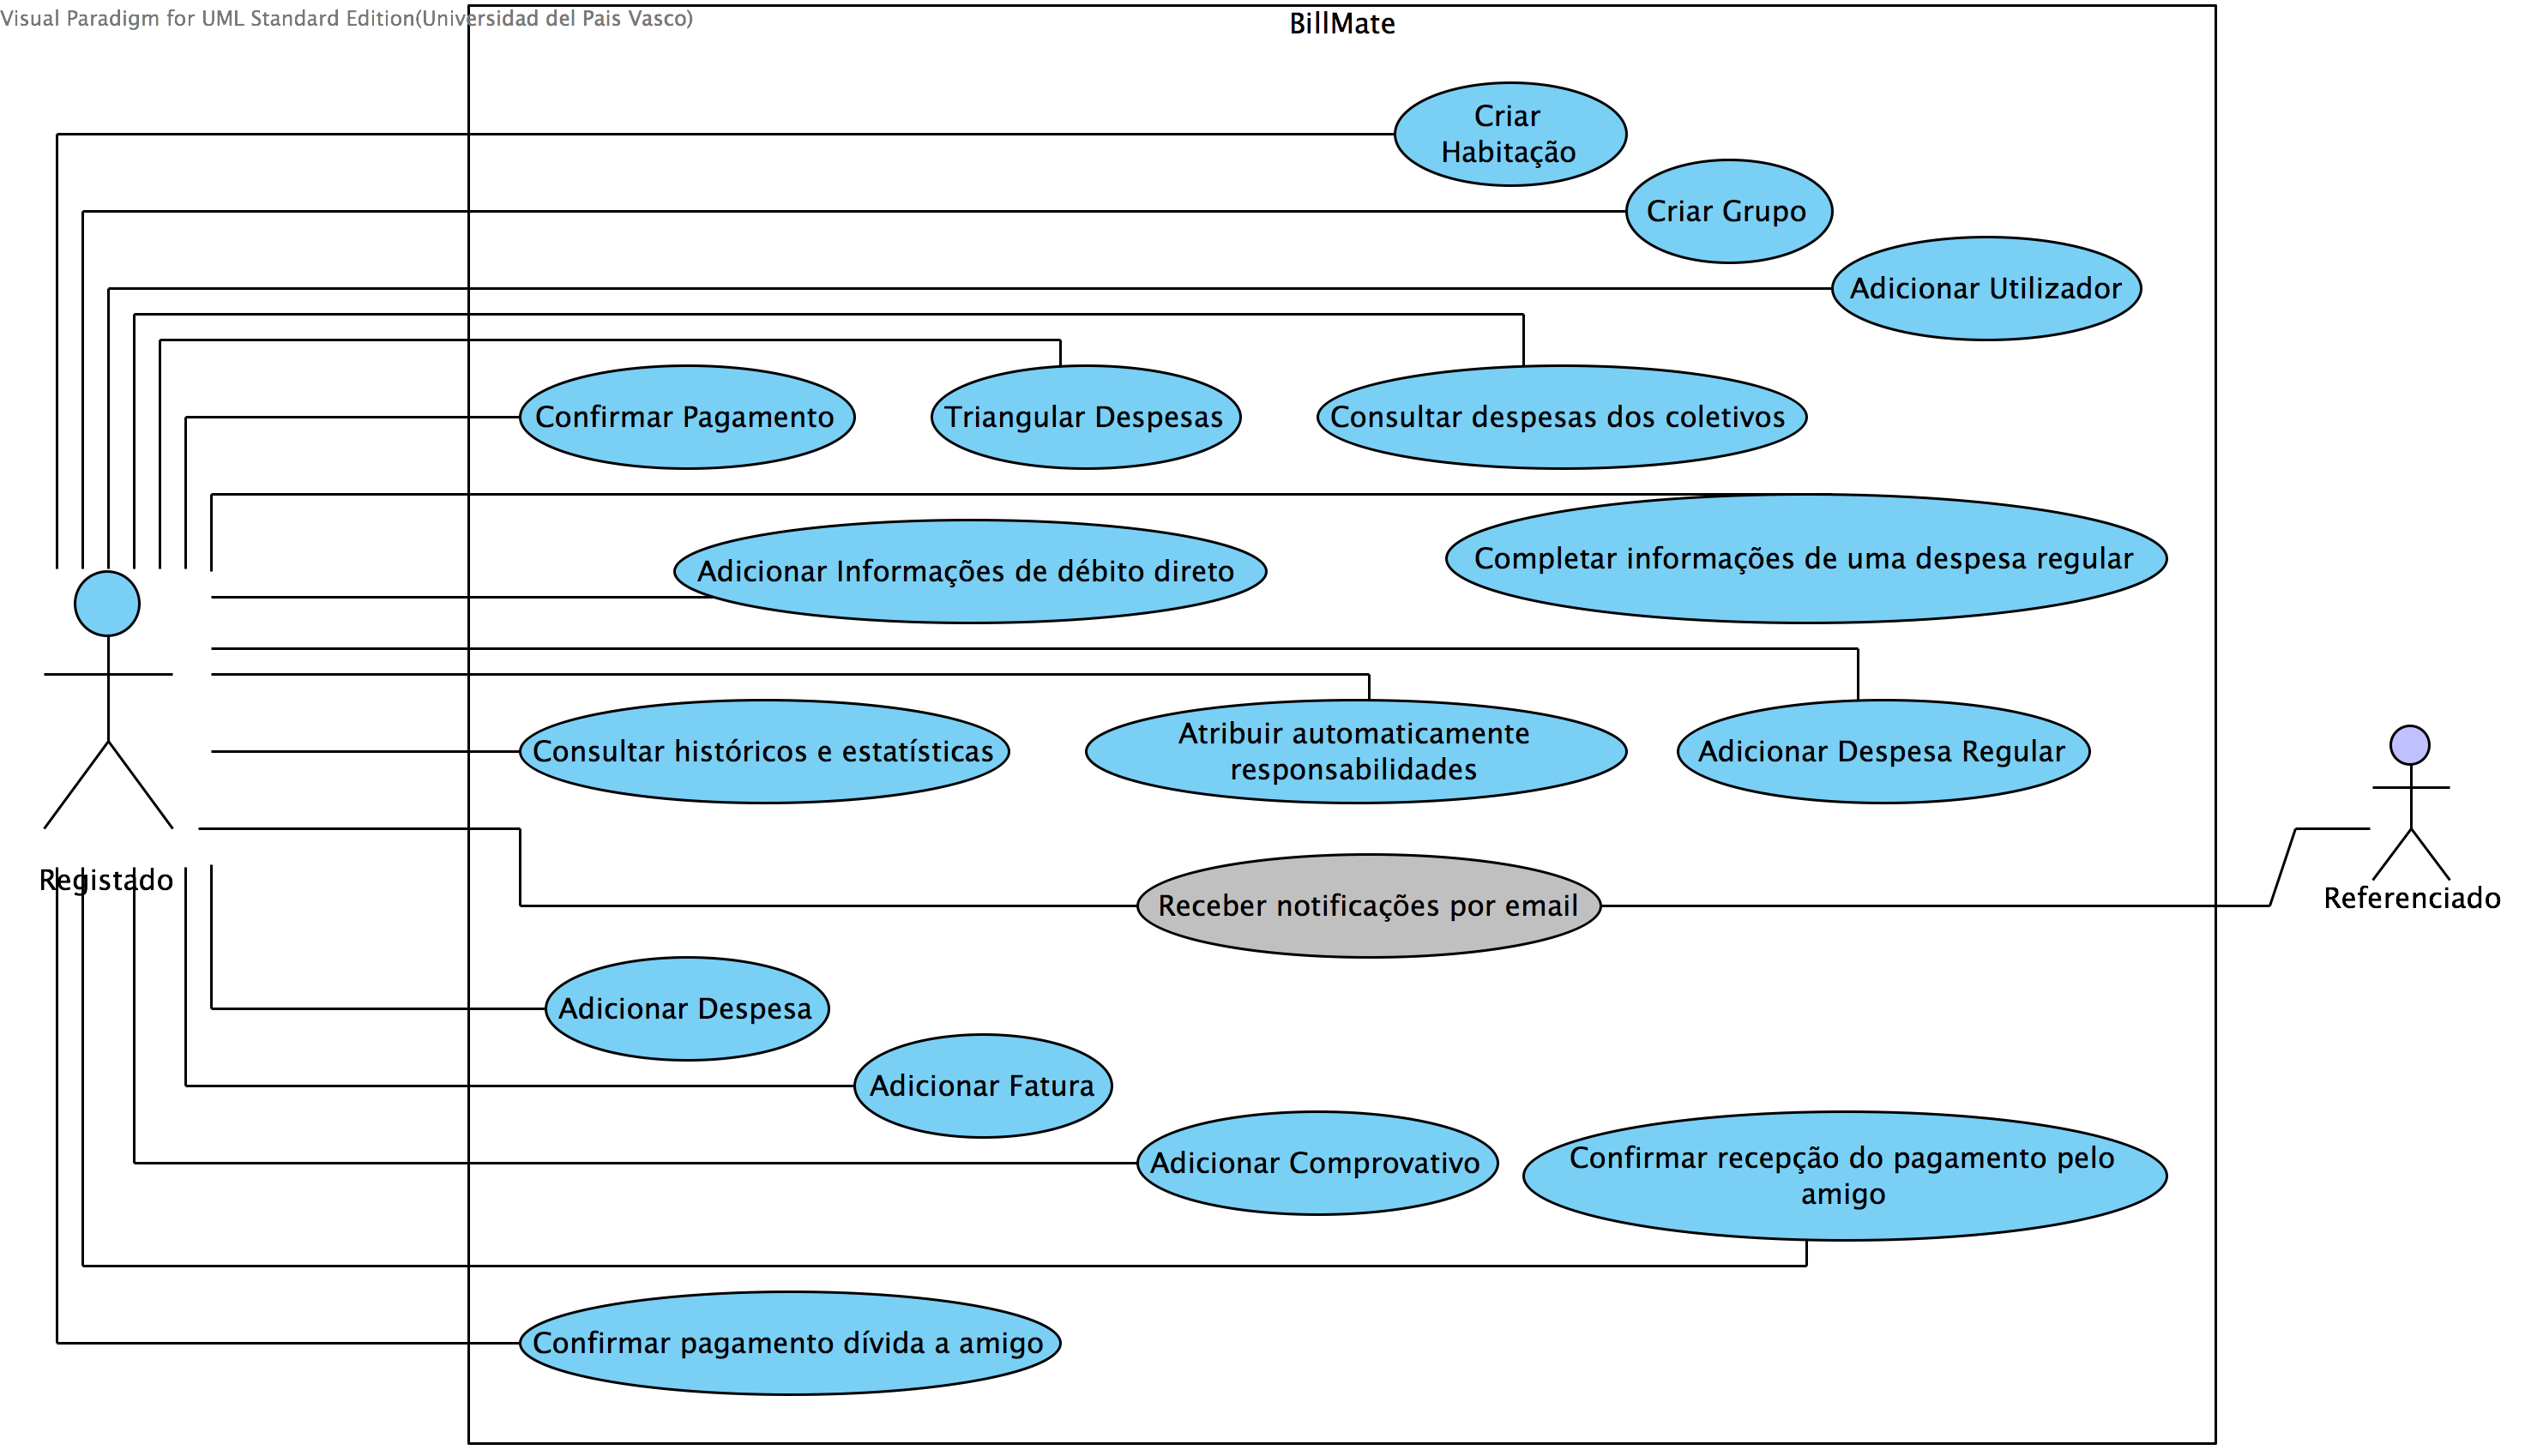
\includegraphics[width=1\textwidth]{images/modeling/useCase}}
\caption{Diagrama de use case}
\end{figure}

\section{Diagrama de Modelo de Domínio}

Tal como o próprio nome indica, domínio, é utilizado para denotar áreas funcionais dentro de sistemas que exibem funcionalidades similares. Este diagrama pode ser interpretado como sendo uma coleção de componentes de software que partilham um determinado conjunto de características.

O objetivo desta análise deve-se ao facto de se puder analisar a informação que é identificada, capturada e organizada, para que se possa reutilizar na interação entre os domínios. É certo que esta reutilização está a ser vista a um nível de abstração muito elevado, uma vez que neste momento apenas se está a analisar o domínio, mas é útil aquando da construção do diagrama de classes. Apesar de não ser este o objetivo, esta modelação será útil se for necessário que as funcionalidades sejam reutilizadas para múltiplos sistemas. \\

\begin{figure}[H]
\centerline{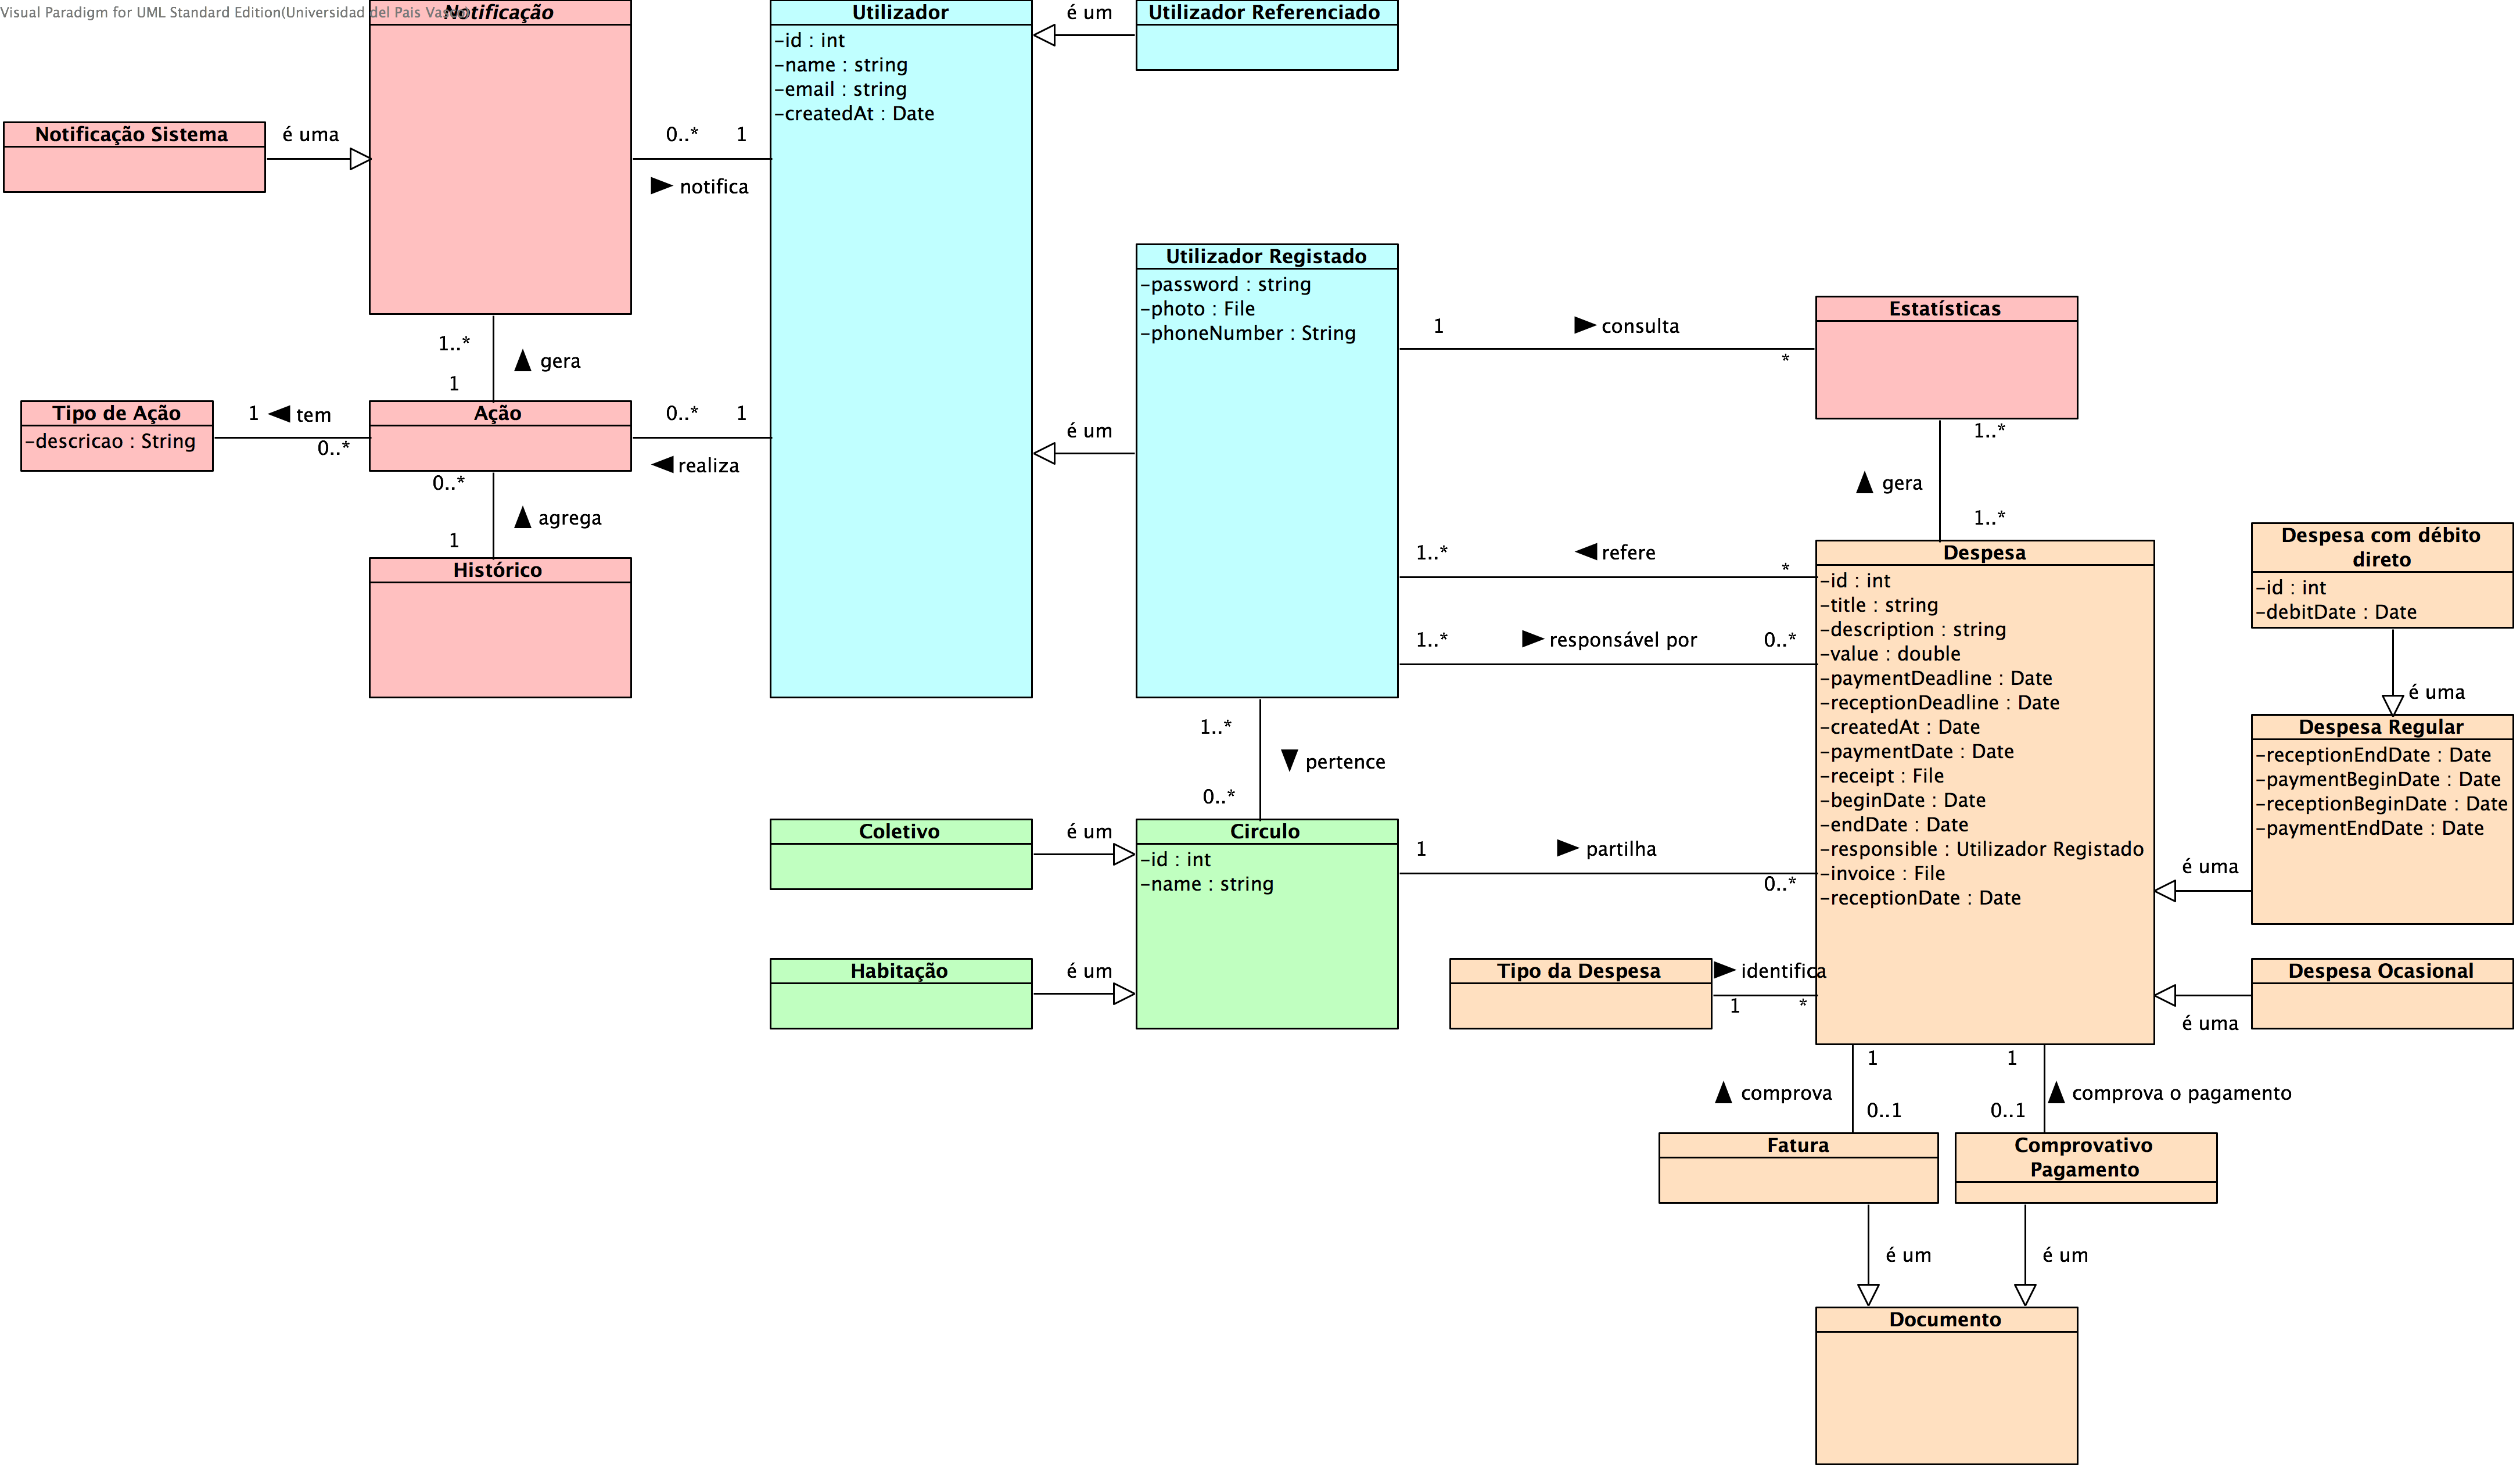
\includegraphics[width=1\textwidth]{images/modeling/modeloDominio}}
\caption{Diagrama do modelo de domínio}
\label{fig:domainModel}
\end{figure}

Tal como se pode analisar pela imagem \ref{fig:domainModel}, um utilizador é uma das entidades principais do sistema, uma vez que é este que despoleta as ações. Este utilizador pode ser classificado como registado ou referenciado. Este distinção deve-se ao facto de um utilizador não ser registado e puder ser utilizado na aplicação para partilhar despesas.
Cada utilizador encontra-se em um ou vários círculos, sendo que um círculo pode ser classificado como um tipo específico (casa), e um tipo mais genérico (colectivos).
Um determinado utilizador que se encontra em um determinado círculo tem despesas, que são partilhadas com os restantes utilizadores daquele mesmo círculo.
Definiu-se o tipo despesa no modelo de domínio, de modo a agrupar as despesas por categorias, sendo elas por exemplo, de eletricidade, de gás, entre outras, que podem até ser personalizadas.
As despesas regulares são criadas para alertar os utilizadores quando se aproxima a data de receção da fatura. Esta data, terá de ser obviamente definida pelo utilizador, que além desta data define a periodicidade com que esta se repete, normalmente mensal, mas é personalizável.
Cada despesa pode ter uma fatura e um recibo, assim como um débito direto.
Todas as ações que são feitas pelos utilizadores, geram notificações para darem feedback constante ao utilizador.

\section{Diagrama de Classes}



\chapter[Interface]
{Interface}

O processo de conceção da interface do utilizador é dividida em \emph{Wireframing e Prototyping}. Em ambos, pretende-se demonstrar interação do utilizador com a aplicação, aumentar a usabilidade e assegurar as seguintes habilidades:
\begin{description}
	\item[Fácil aprendizagem] O utilizador requer pouco treino para usufruir da aplicação
	\item[Fázil de memorizar] Reduzir o esforço de memória por parte do utilizador
	\item[Máximizar a produtividade] O utilizador deve executar uma tarefa de forma rápida e eficaz
	\item[Minimizar erros] A aplicação deve evitar a ocorrência e auxiliar na resolução destes caso ocorram
	\item[Maximizar satisfação] A aplicação transmite confiança e segurança
\end{description}
\section{Wireframing}

A primeira fase de conceção da interface, consistiu na elaboração de \emph{Wireframes}, protótipos de baixa fidelidade, que tiveram como objetivos:

\begin{itemize}
	\item Identificar funcionalidades do sistema
	\item Identificar cenários complexos
	\item Compreensão de fluxos e processos
	\item Abtração das questões estéticas
\end{itemize}

Para além dos objetivos, houve a preocupação de saber a opinião de outras pessoas, que se enquadram no público alvo a quem se destina o \emph{BillMate}

Para a conceção de \emph{Wireframes}, recorreu-se à aplicação \emph{Web} \emph{Moqups}. Na figura ~\ref{fig:mockup_dashboard} está representado o \emph{Wireframe} correspondente à \emph{Dashboard} quando acedida a partir de um \emph{browser}. Sendo esta a página mais importante da aplicação, houve um cuidado em aplicar ao máximo padrões sobre interfaces. Os padrões que mais se destacam são:

\begin{itemize}
	\item \emph{Dashboard}
	\item \emph{Accordions}
	\item \emph{Modals}
\end{itemize}

\begin{figure}[ht]
\centering
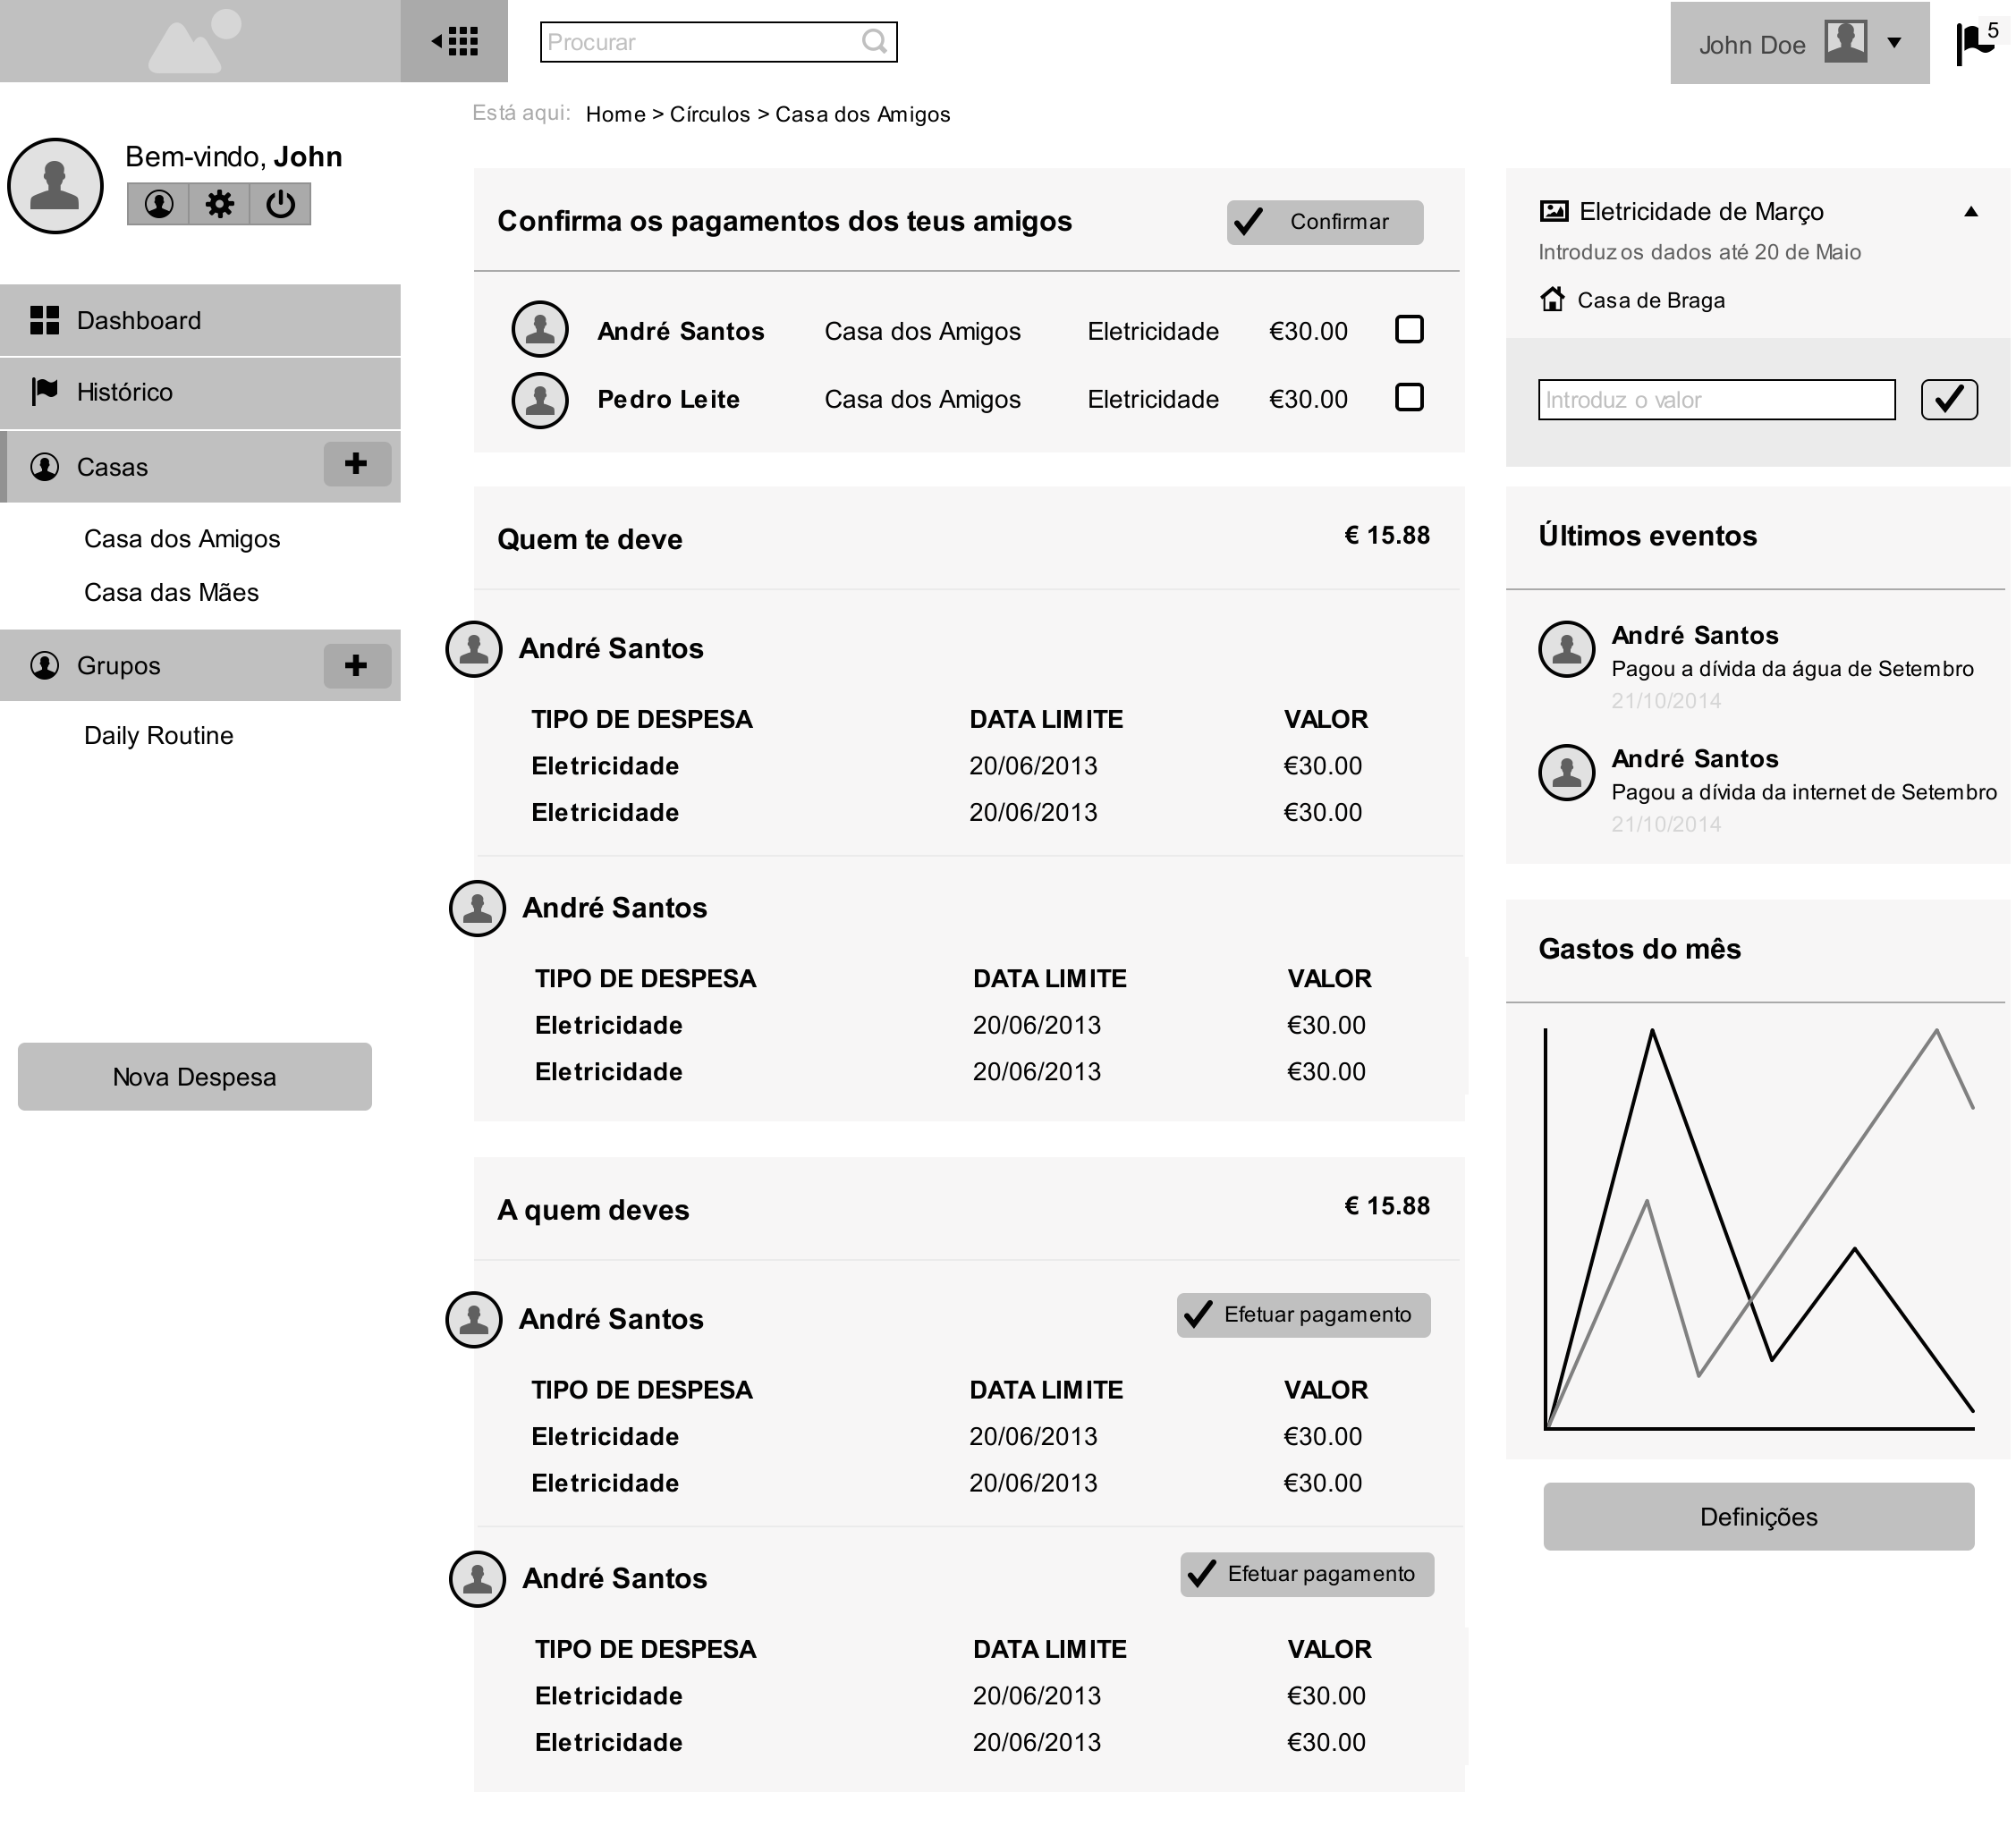
\includegraphics[width=.9\textwidth]{images/mockup_dashboard}
\caption{Dashboard vista a partir de um \emph{browser}}
\label{fig:mockup_dashboard}
\end{figure}

Nesta mesma fase, houve a preocupação de conceber a aplicação para outros equipamentos e que esta se adapta-se à ecrãs de diferentes tamanhos.

Na figura ~\ref{fig:mockup_mobile} está o \emph{Wireframe} correspondente à \emph{Dashboard} quando acedida a partir da aplicação \emph{mobile}. Nesta aplicação, as principais preocupações foram:

\begin{itemize}
	\item Mater a semelhança com a aplicação \emph{Web},
	\item Reaproveitar a barra lateral para organizar conteúdo sob a forma de lista (como é o caso das casas e dos grupos)
	\item Converter modais em novas janelas
	\item As funcionailidades principais passam a estar disponiveis numa barra de navegação no fundo da página
\end{itemize}

\begin{figure}[ht]
\centering
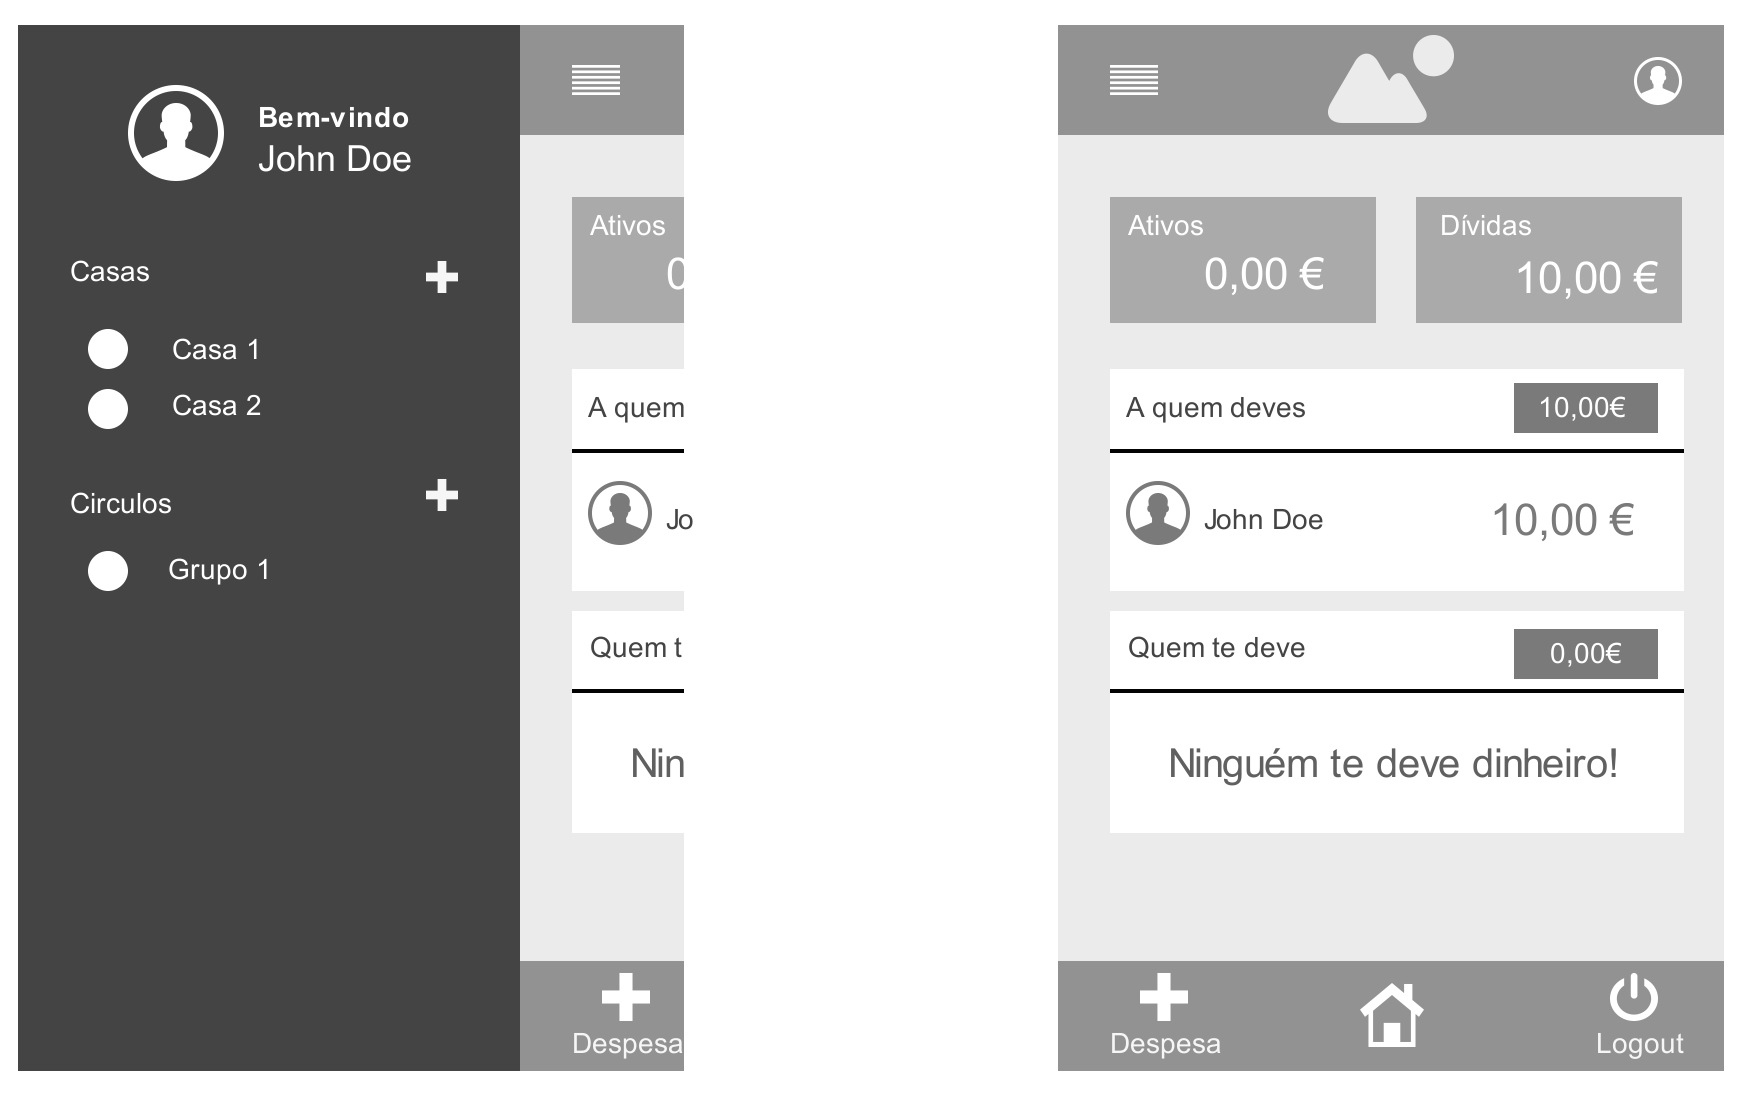
\includegraphics[width=.9\textwidth]{images/mobilemockup}
\caption{Dashboard vista a partir da aplicação \emph{mobile}}
\label{fig:mockup_mobile}
\end{figure}



\section{Prototipagem}

Nesta fase de conceção da interface do utilizador, começou-se a dar mais importantia as questões estéticas. Criou-se então protótipos com recurso a \emph{HTML CSS e JavaScript}. Houve também uma nova avaliação à usabilidade da mesma.

Quanto a adaptação da interface à ecrãs de diferentes tamanhos, utilizou-se o sistema de \emph{grids} do\emph{Bootstrap}, uma \emph{framework} de \emph{CSS e JavaScript}.

Na figura ~\ref{fig:proto_dash} está o protótipo correspondente à \emph{Dashboard} quando acedida a partir de um \emph{browser} num ecrã \'comum\' e na figura ~\ref{fig:proto_mobile} está o \emph{protótipo} correspondente à \emph{Dashboard} quando acedida a partir da aplicação \emph{mobile}.

\begin{figure}[ht]
\centering
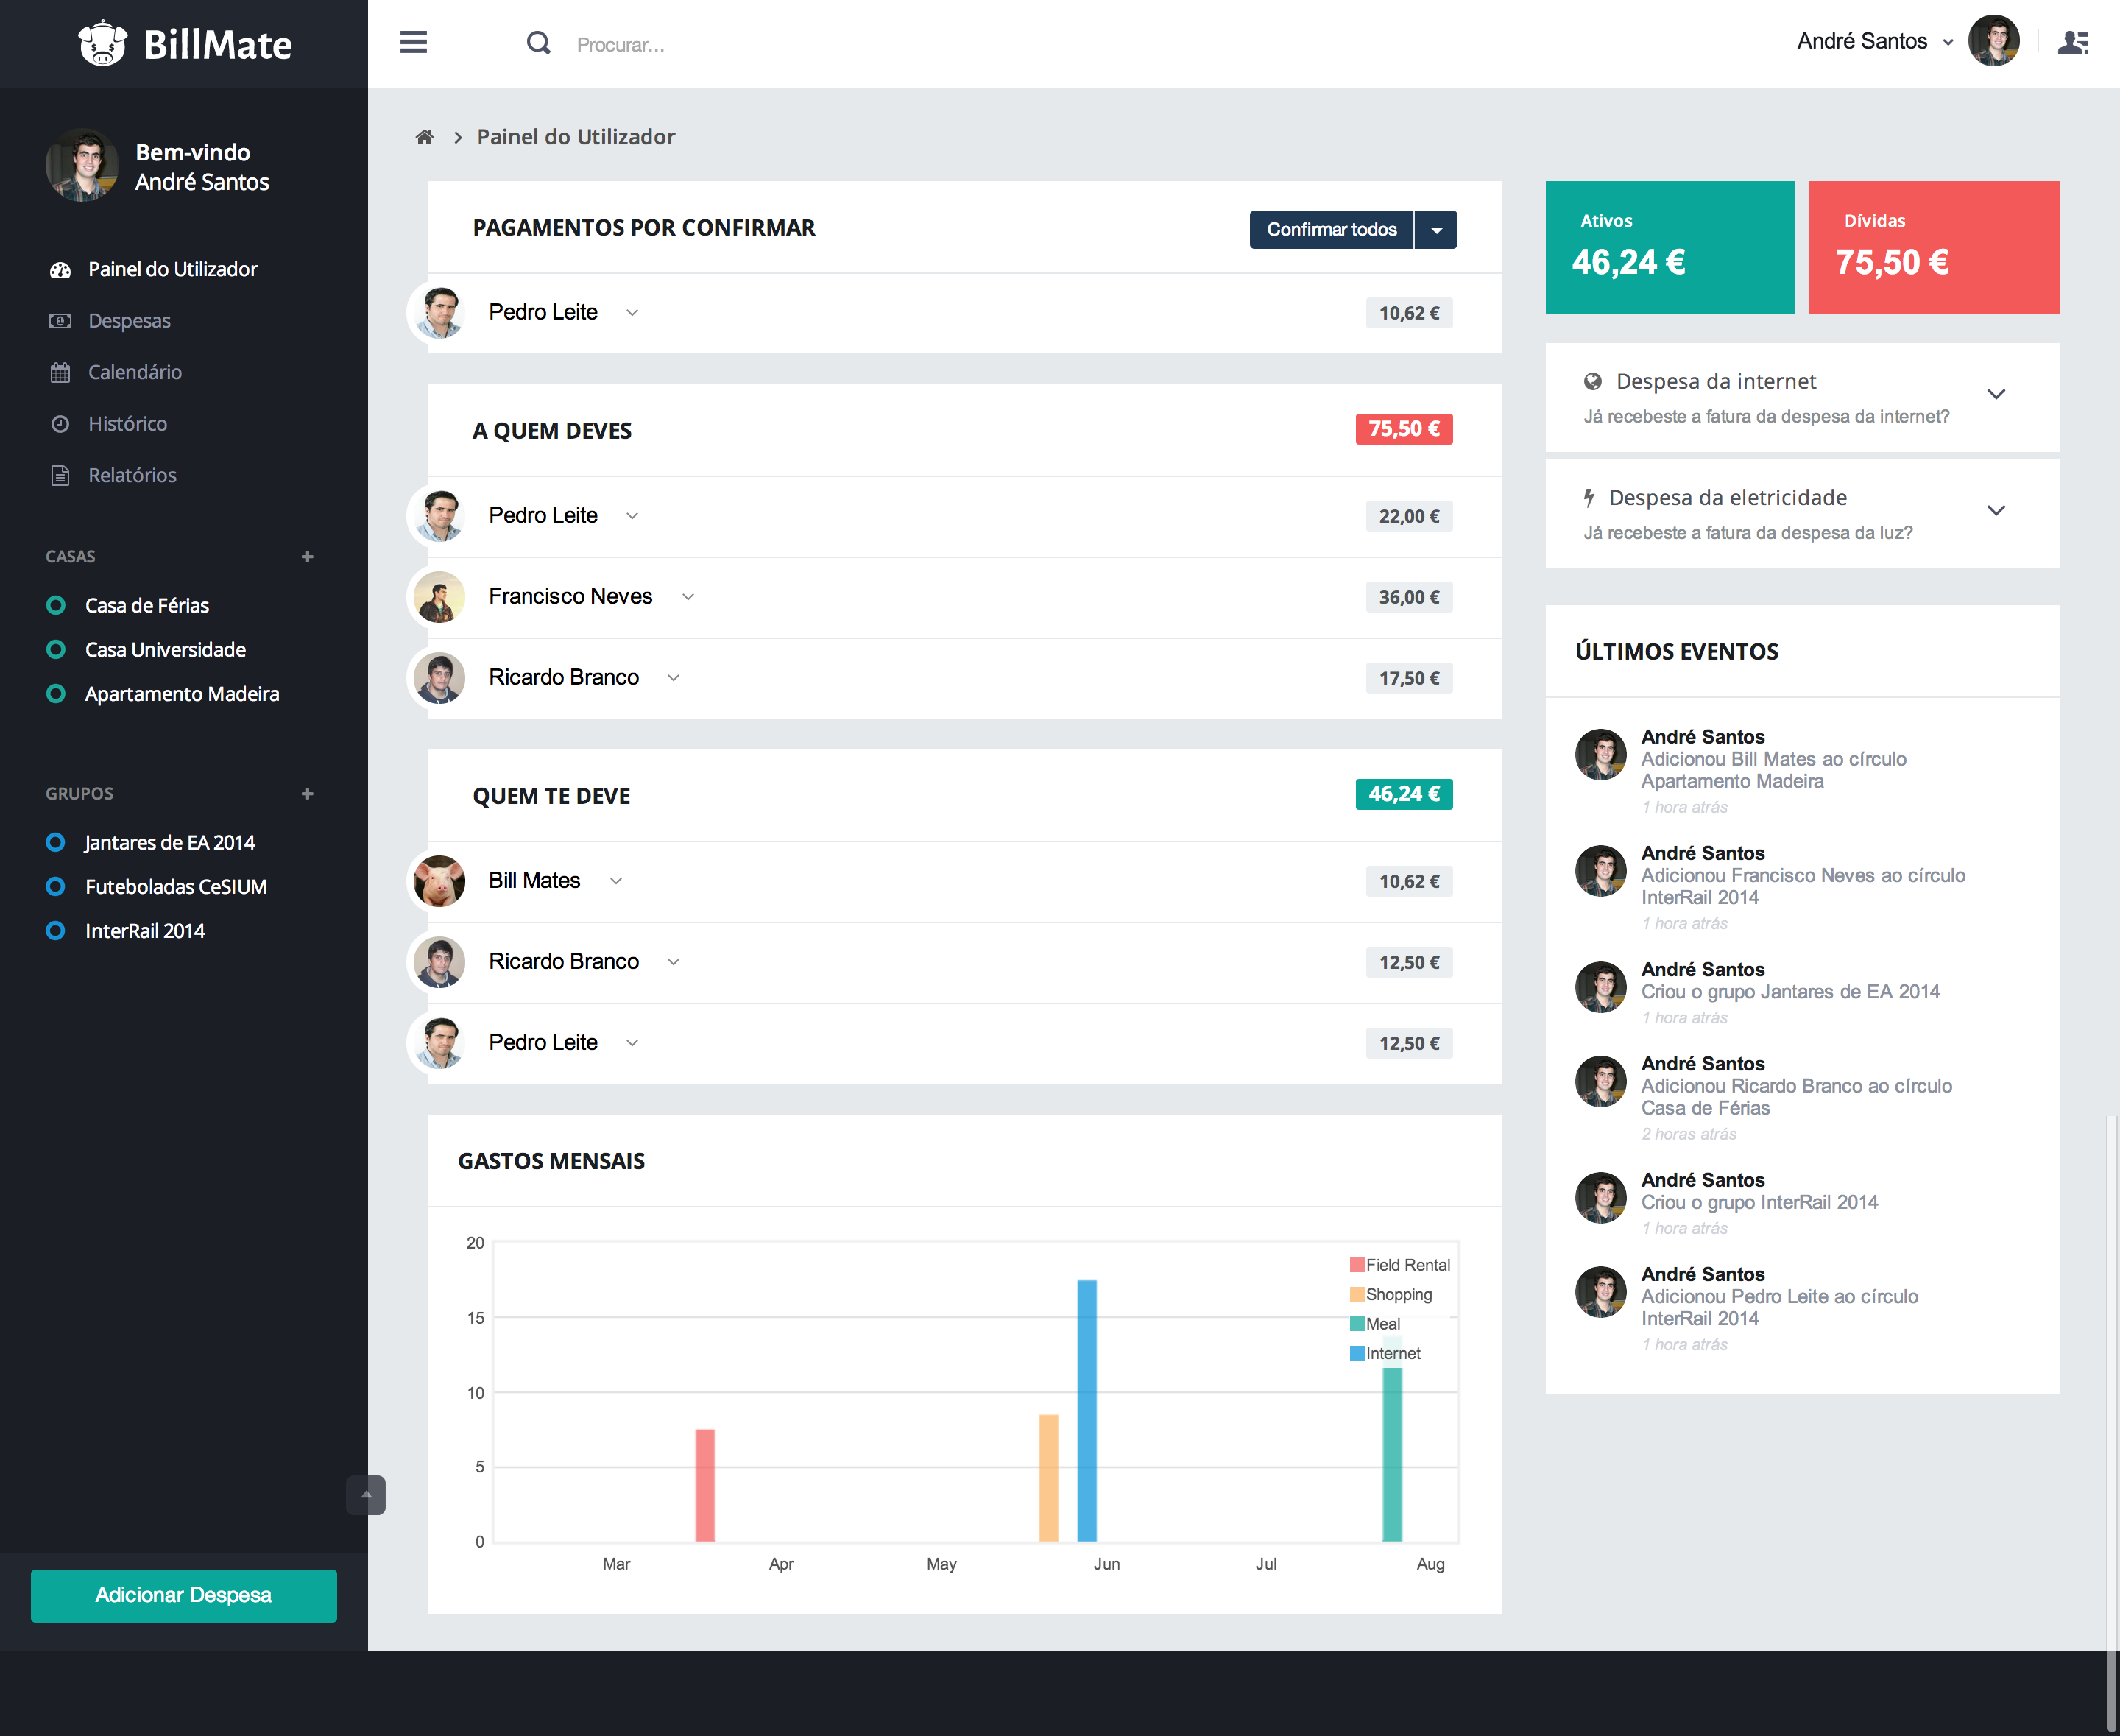
\includegraphics[width=.9\textwidth]{images/dashboardprot}
\caption{Dashboard vista a partir do \emph{browser}}
\label{fig:proto_dash}
\end{figure}


\begin{figure}[ht]
\centering
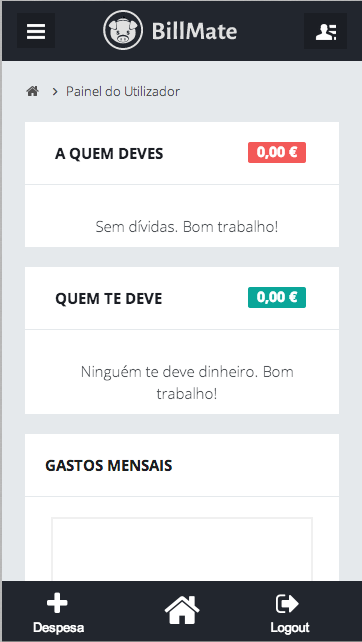
\includegraphics[width=.9\textwidth]{images/protmobile}
\caption{Dashboard vista a partir da aplicação \emph{mobile}}
\label{fig:proto_mobile}
\end{figure}


\chapter[Implementação]
{Implementa\c{c}\~ao}



\section{Tecnologias}

\section{Servidor}

\input{sections/implementation/technologies/server/webFramework}
\input{sections/implementation/technologies/server/database}

\subsection{Cliente}



\chapter[Análise de desempenho]
{An\'alise de desempenho}

Uma vez concretizada a infraestrutura e o \emph{deploy} da aplicação, é necessário analisar o desempenho do serviço, recorrendo a métodos de geração de dados, a rotinas de testes e iterações de modo a obter resultados que possam fundamentar medidas a tomar.

O objectivo da análise de desempenho é perceber até que ponto o serviço escala sem ocorrerem problemas e quais são os \emph{bottlenecks}, caso existam de uma forma explícita, que contribuem para o contrário.

\section{Povoação da base de dados}

Por forma a incluir alguma carga de registos no serviço, tais como utilizadores, círculos, despesas e pagamentos, optou-se por implementar um \emph{script} na linguagem \emph{PHP}.


A linha de pensamento seguida foi:
\begin{itemize}
	\item \textbf{Adicionar utilizadores no sistema} \\
		\indent A adição de utilizadores é necessária, visto que todo o resto do procedimento de geração de dados se torna dependente destes. Para obter a lista de utilizadores, recorreu-se à \emph{API} do \emph{www.randomuser.me}. Para registar utilizadores no sistema, usou-se o seguinte comando:
		\begin{verbatim}
			php seedRegisteredUser.php <quantity>
		\end{verbatim}

	\item \textbf{Adicionar círculos de utilizadores} \\
		\indent Tendo em conta que, no sistema, os círculos são os pontos de encontro de utilizadores, torna-se essencial gerar alguns de modo a que possam interagir através da adição de despesas e os respetivos pagamentos.
		\begin{verbatim}
			php seedCircle.php <quantity>
		\end{verbatim}

	\item \textbf{Adicionar despesas aos círculos} \\
		\indent Tendo em conta que, no sistema, os círculos são os pontos de encontro de utilizadores, torna-se essencial gerar alguns de modo a que possam interagir através da adição de despesas e os respetivos pagamentos.
		\begin{verbatim}
			php seedExpense.php <quantity_per_circle>
		\end{verbatim}

	\item \textbf{Adicionar pagamentos de despesas} \\
		\indent Para simular algum estado com algumas alterações, foram simulados pagamentos de despesa, de modo a verificar diferentes estados da aplicação.
		\begin{verbatim}
			php seedPayment.php
		\end{verbatim}
\end{itemize}

Note que os estados intermédios de cada comando são recolhidos do estado da base de dados e guardados localmente, no formato \emph{JSON}.

Desta forma, depois de inseridos os estados, pode dar-se início à rotina de recolha de dados sobre o comportamento do sistema face às cargas a que é sujeito, que será explicada de seguida.

\section{Rotina}

Como se referiu anteriormente, foi seguida uma rotina para a execução do \emph{benchmark}, que consiste na tomada de vários passos para obter os resultados do desempenho do sistema. Antes de iniciar a rotina, é reposto o estado inicial da base de dados, ou seja, o estado final após a geração de dados.

Fez-se uso da ferramenta \emph{Apache Bench}, cujo objectivo, como o nome indica, é efetuar um determinado número de pedidos ao \emph{URL} que lhe é passado, neste caso o da \emph{dashboard} do utilizador, onde o custo de carregamento de todos os \emph{widgets} nela incluídos se torna interessante de pôr em questão. Os passos tomados na rotina foram os seguintes:

\begin{itemize}
	\item Execução de um aquecimento prévio da base de dados;
	\item Execução do \emph{Apache Bench} para 500 pedidos com 8 clientes concorrentes;
	\item Execução do \emph{Apache Bench} para 500 pedidos com 16 clientes concorrentes;
	\item Execução do \emph{Apache Bench} para 500 pedidos com 32 clientes concorrentes;
	\item Geração de gráficos.
\end{itemize}

\section{Ambiente de teste}

Antes de iniciar os testes, foi preparado o seguinte ambiente de teste:

\begin{itemize}
	\item \emph{\emph{Router}} por cabo com \textit{~1.3ms} de latência
	\item \textbf{Quatro computadores:}
		\begin{itemize}
			\item \textbf{MacBook Pro 13" Late 2013}
				\begin{itemize}
					\item Core i5 (I5-4258U) 2.6GHz
					\item 16GB RAM
					\item 256GB SSD
					\item \textbf{Suporta:} \emph{Web Servers, Application Servers}
				\end{itemize}

			\item \textbf{MacBook Pro 13" Retina 2012}
				\begin{itemize}
					\item Core i5 (I5-3210M) 2.5GHz
					\item 8GB RAM
					\item 128GB SSD
					\item \textbf{Suporta:} \emph{Storage, Service Cluster}
				\end{itemize}

			\item \textbf{MacBook Air 13" 2012}
				\begin{itemize}
					\item Core i5 (I5-3427U) 1.8GHz
					\item 4GB RAM
					\item 128GB SSD
					\item \textbf{Suporta:} \emph{Application Cache Servers, Load Balancers}
				\end{itemize}

			\item \textbf{MacBook Pro 15" (Unibody)}
				\begin{itemize}
					\item Core 2 Duo (T9400) 2.53 GHz
					\item 4GB RAM
					\item 256GB SSD
					\item \textbf{Suporta:} \emph{Apache Bench, Load Balancers}
				\end{itemize}
		\end{itemize}
\end{itemize}

As diferenças a nível de características podem influenciar os resultados dos testes. Na secção seguinte, serão discutidos os resultados obtidos.

\section{Iterações}

Por forma a perceber qual o comportamento da aplicação na infraestrutura que a suporta, aplicou-se o \emph{benchmark} a várias iterações, alterando o número de \emph{Application Servers}, usufruindo da capacidade de escalar horizontalmente esta componente.

Inicialmente procedeu-se a uma otimização da base de dados, como será visto de seguida.

\subsection{Otimização da Base de Dados}

A base de dados é gerada durante o \emph{deployment} da aplicação no servidor aplicacional. Como o \emph{Hibernate} não tem conhecimento da aplicação, não é da responsabilidade do mesmo adicionar índices nem otimizar a base de dados.

A figura seguinte relata os resultados pré-otimização e pós-otimização com dois servidores aplicacionais.

\begin{figure}[H]
\centerline{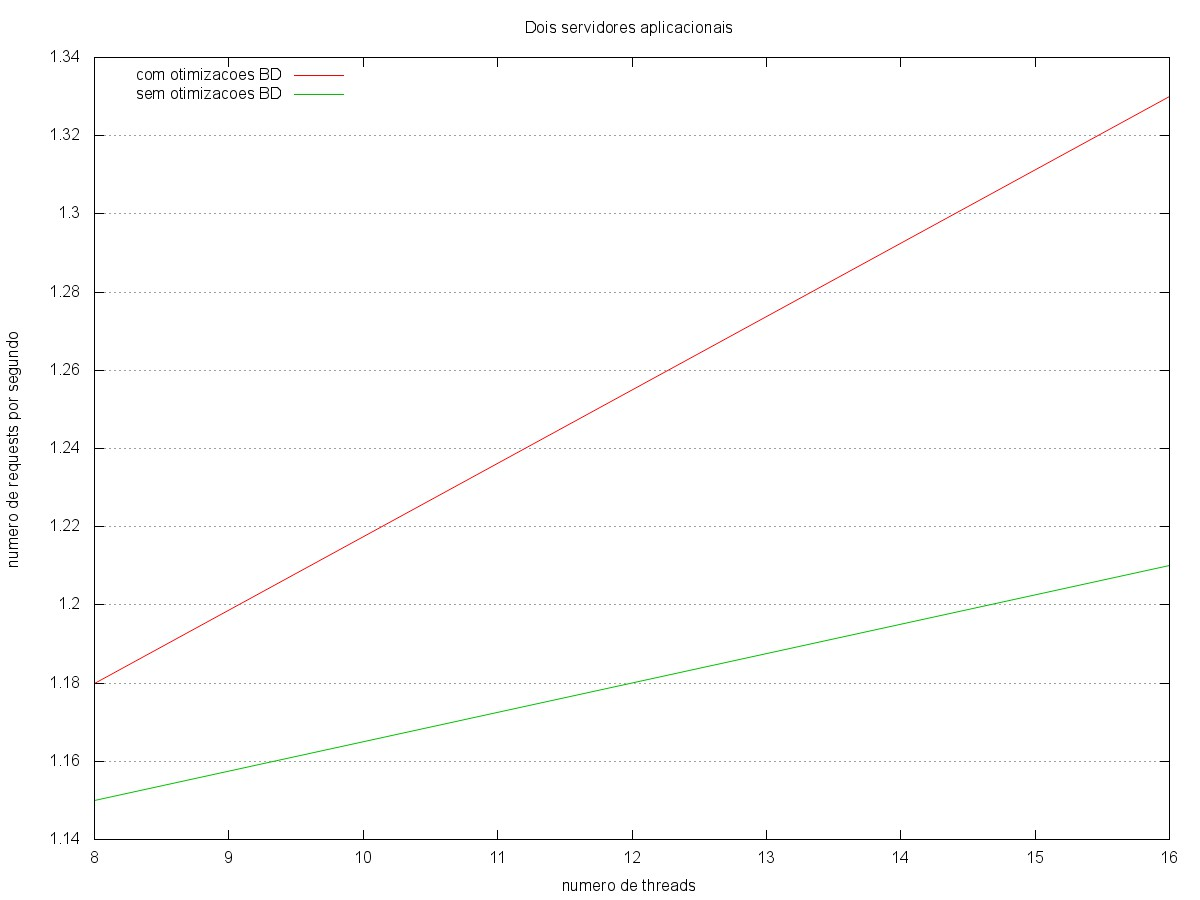
\includegraphics[width=1\textwidth]{images/benchmark/optimization}}
\label{fig:optimization}
\caption{Resultados obtidos antes e depois da otimização}
\end{figure}

Repare que, com otimização, a situação não é tão grave como sem otimização. Para atingir este objetivo, atentou-se nas \emph{queries} efetuadas com mais de \emph{10ms} de tempo de execução, adicionaram-se índices e ordenaram-se algumas tabelas de acordo com alguns deles.

Obtendo-se estes resultados, usou-se a configuração para os testes seguintes.

\subsection{Application Servers}

Prosseguindo os testes com as configurações da base de dados, foi executada a rotina para dois, três e quatro servidores aplicacionais. Não foi executada para mais servidores devido à falta de recursos.

\begin{figure}[H]
\centerline{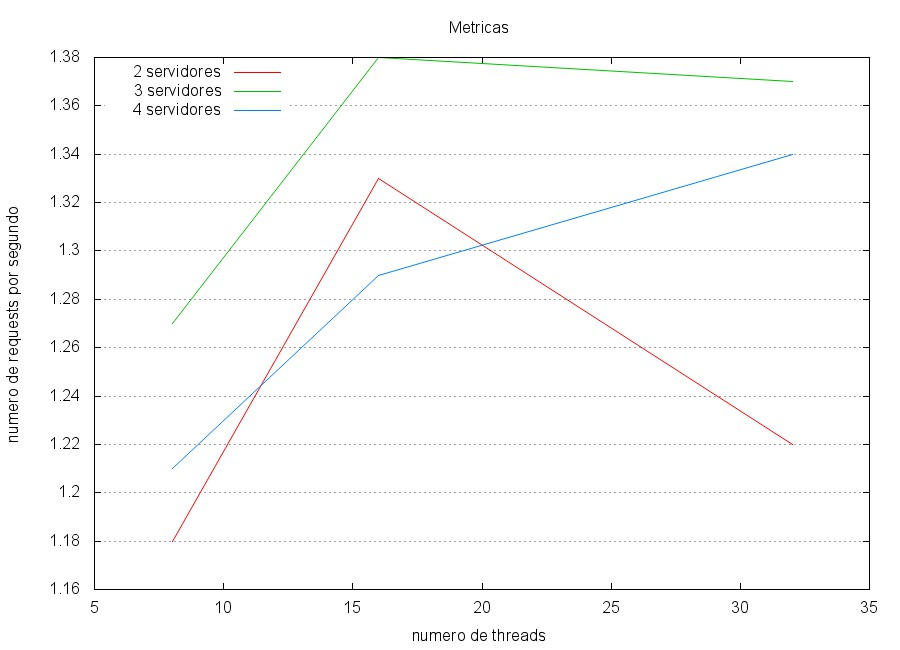
\includegraphics[width=1\textwidth]{images/benchmark/servers}}
\caption{\emph{Benchmark} para dois, três e quatro servidores}
\end{figure}


Como se verifica, a aplicação tem uma grande dificuldade em escalar. O aumento de dois para três servidores aplicacionais resolveu parte do problema, permitindo uma melhoria no desempenho. No entanto, não sendo aquilo que se esperava, adicionar um \emph{Application Server} torna tudo mais lento inicialmente, embora no final do gráfico este continue a crescer. Note, também, que a partir dos 32 clientes o gráfico deixa de existir, devido à falta de recursos para suportar mais do que os referidos. Por acréscimo, as máquinas responsáveis pela \emph{Storage} tiveram um uso de cerca de 30\% de \emph{CPU}.

Tentou-se, também, executar os testes para 64 clientes, mas não se obtiveram resultados, visto que a aplicação atingia o ponto de saturação e o tempo de espera \emph{Apache Bench} alcançava o seu \emph{timeout}.

\section{Conclusões finais}


% \chapter[Trabalho futuro]
{Trabalho futuro}



\chapter[Conclusão e trabalho futuro]
{Conclus\~ao e trabalho futuro}

Após o término do trabalho, é possível denotar alguns aspetos que não correram da melhor maneira, destacando sobretudo o facto do desconhecimento da framework. Com a evolução da implementação, foi se conhecendo novas maneiras de implementar, cada vez mais eficientes, que se fossem desenvolvidas desde o início, poderia se otimizar muito do código implementado.

Deve-se salientar também que a modelação deveria ter sido realizada com mais detalhe, porque a certa altura, teve-se de alterar os domínios do sistema para tornar a aplicação mais eficiente. Esta alteração obrigou a que fosse atualizada bastante da lógica de negócio.
A infraestrutura foi realizada com sucesso, e conseguiu-se ultrapassar os objetivos que foram propostos, mas tem-se consciência que se tivesse havido mais algum estudo sobre os recursos que foram utilizados, conseguiria-se ter menos máquinas a fazer a mesma coisa.

Um ponto negativo que também importa referir, é que os cenários de teste não foram realizados com o rigor que se pretendia, porque esse aspeto é um ponto que deve ser muito bem planeado, e nos quais não foram bem identificados.

Contudo, este trabalho permitiu melhorar algumas competências em programação orientada a objetos, perceber melhor aspetos ligados a \textit{enterprise application} que até este momento eram desconhecidos pela maioria dos elementos do grupo e começar a lidar com problemas reais como testes e \textit{deploy} da aplicação.

Como trabalho futuro, pretende-se melhorar a aplicação, otimizando e fazendo mais testes de integração. Pretende-se ainda implementar funcionalidades adicionais, tal como o triangulação de despesas que foi proposto mas não foi realizado. Terminar a aplicação móvel e lançamento da versão beta.

\begin{bibliografia}


	%\begin{chapreferences}{}
	%\bibitem{ref}NomeAutor,
	%                 {\it NomeLivro}, Editora,
	%                 Cidade, Ano.
	%\end{chapreferences}


\end{bibliografia}

\newpage
\nocite{*}
\bibliographystyle{plain}
\bibliography{www}

\begin{referenciaswww}

\newpage
\appendix{Web dashboard}
\markboth{Web dashboard}{Web dashboard}


\begin{figure}[ht]
\sidebyside{
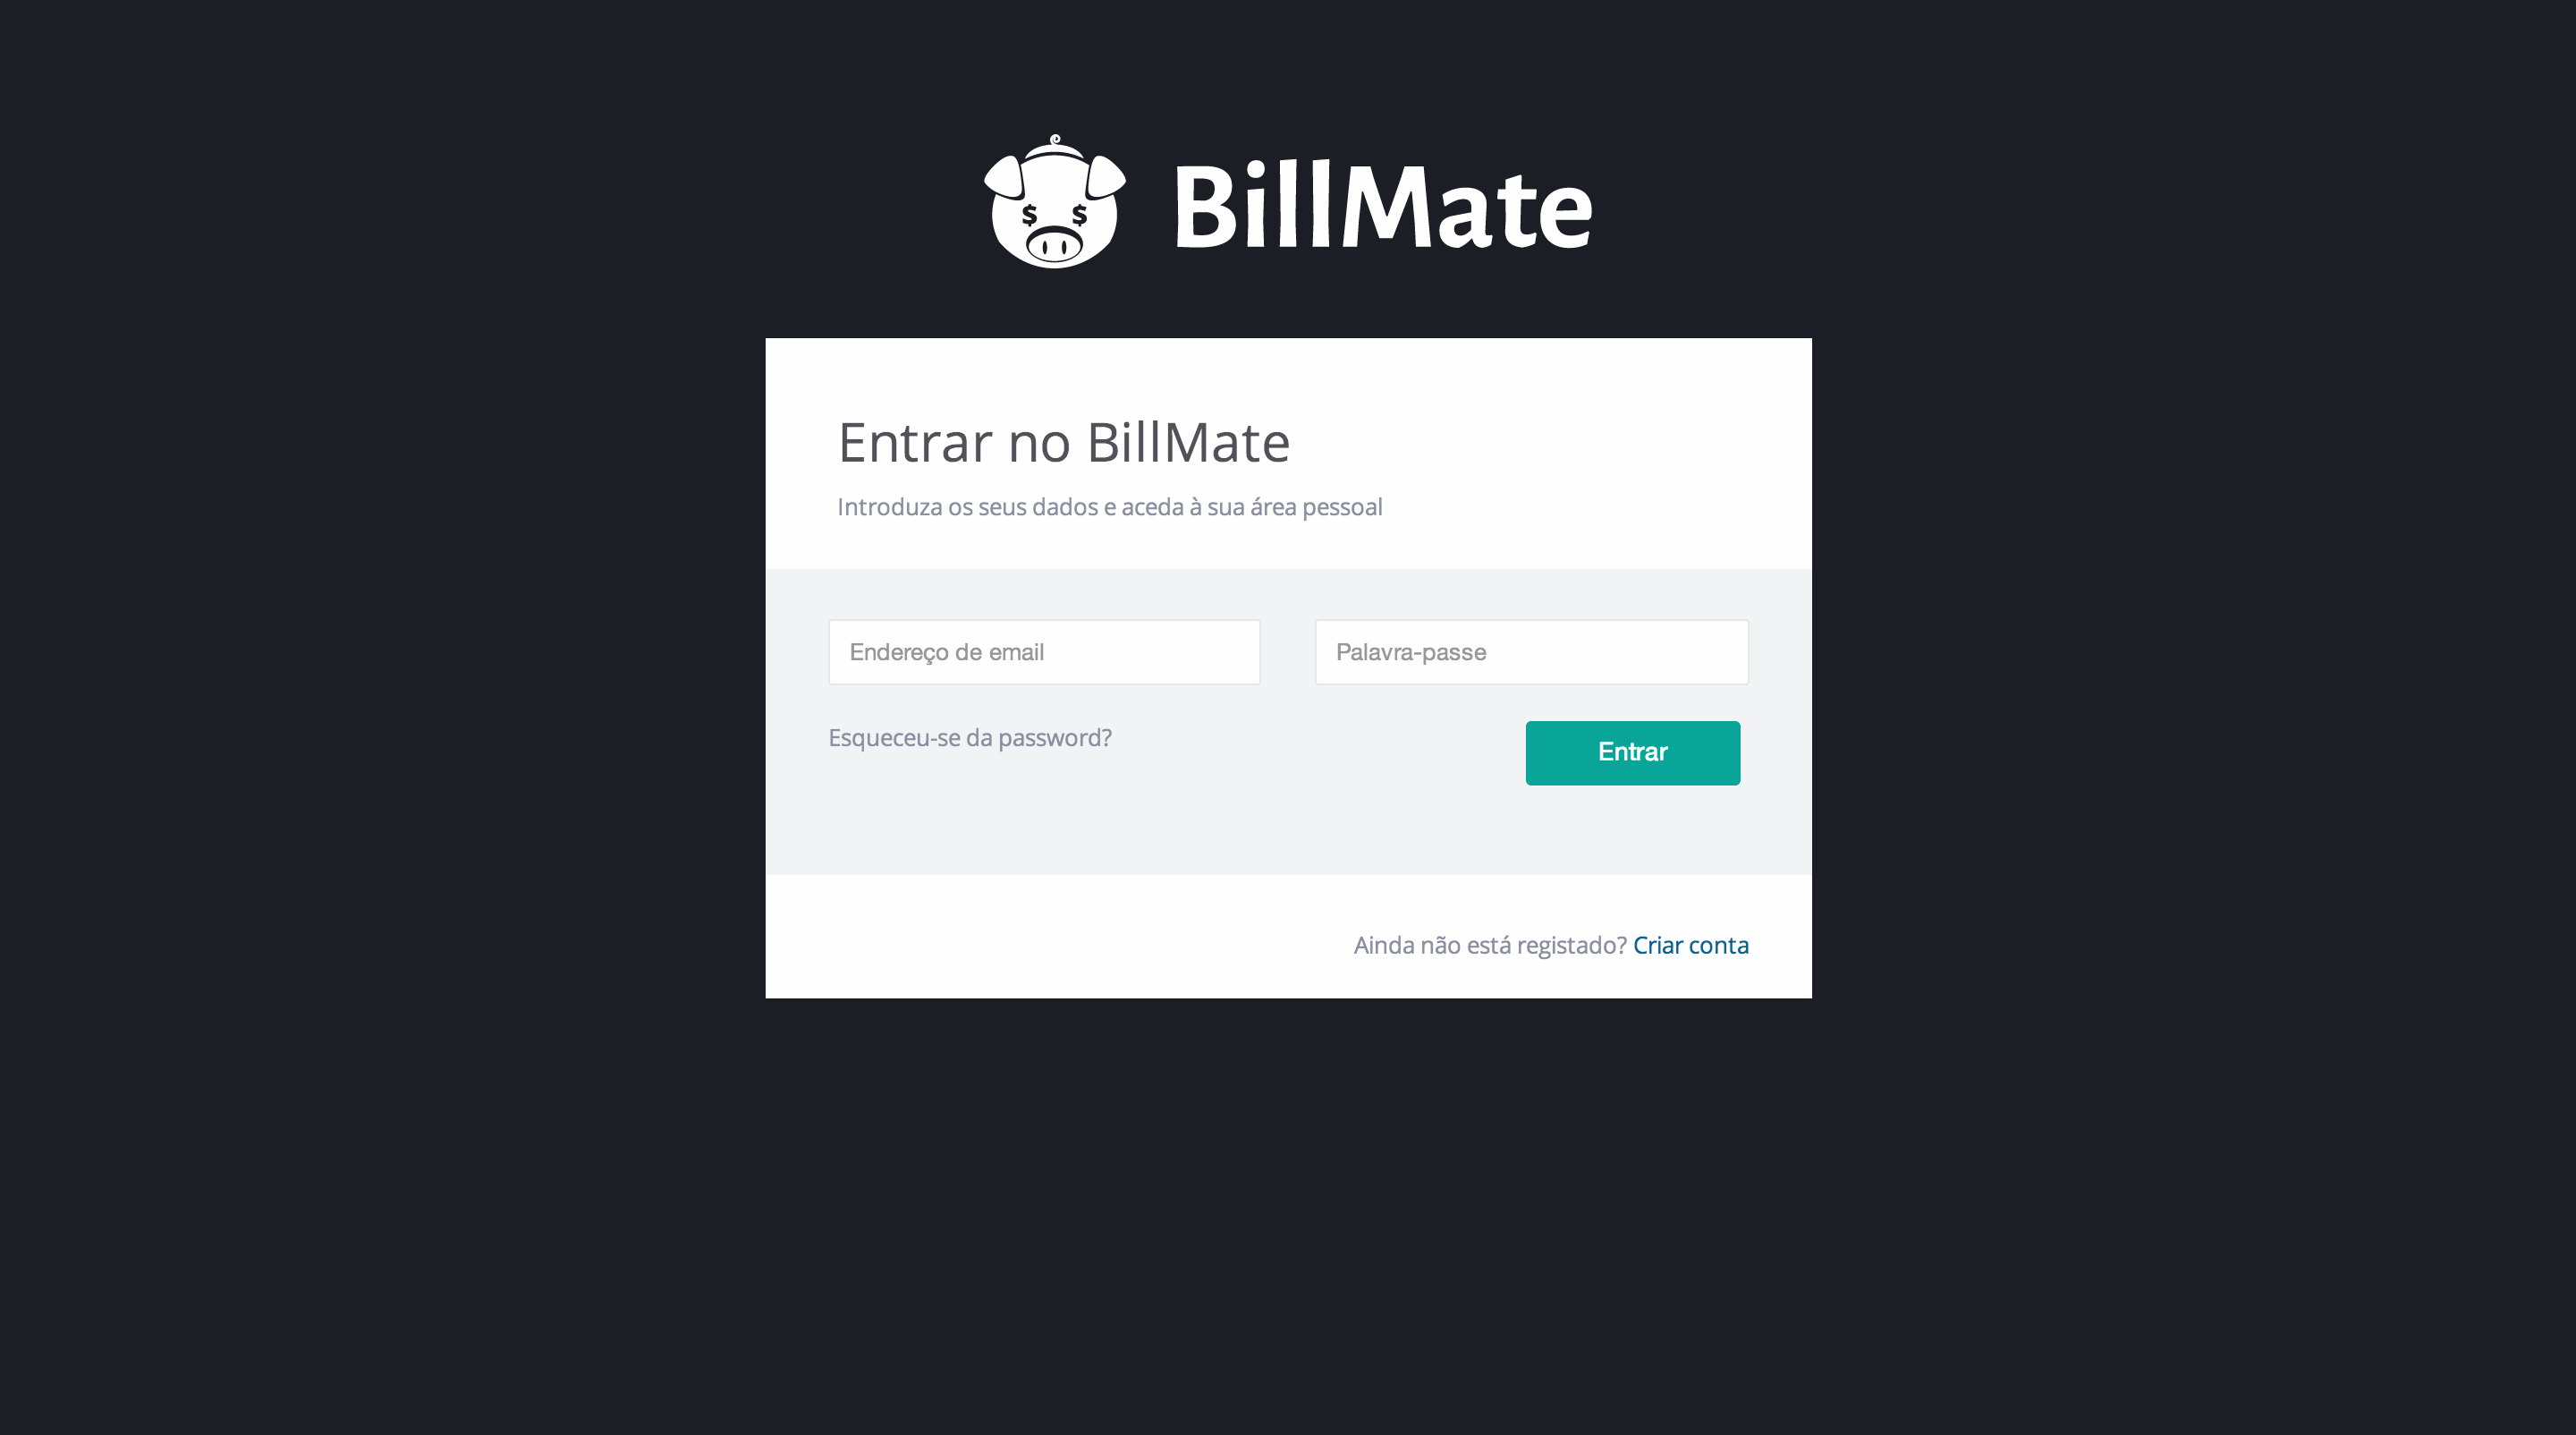
\includegraphics[width=.5\textwidth]{images/andre/login}
\caption{Login}
}
{
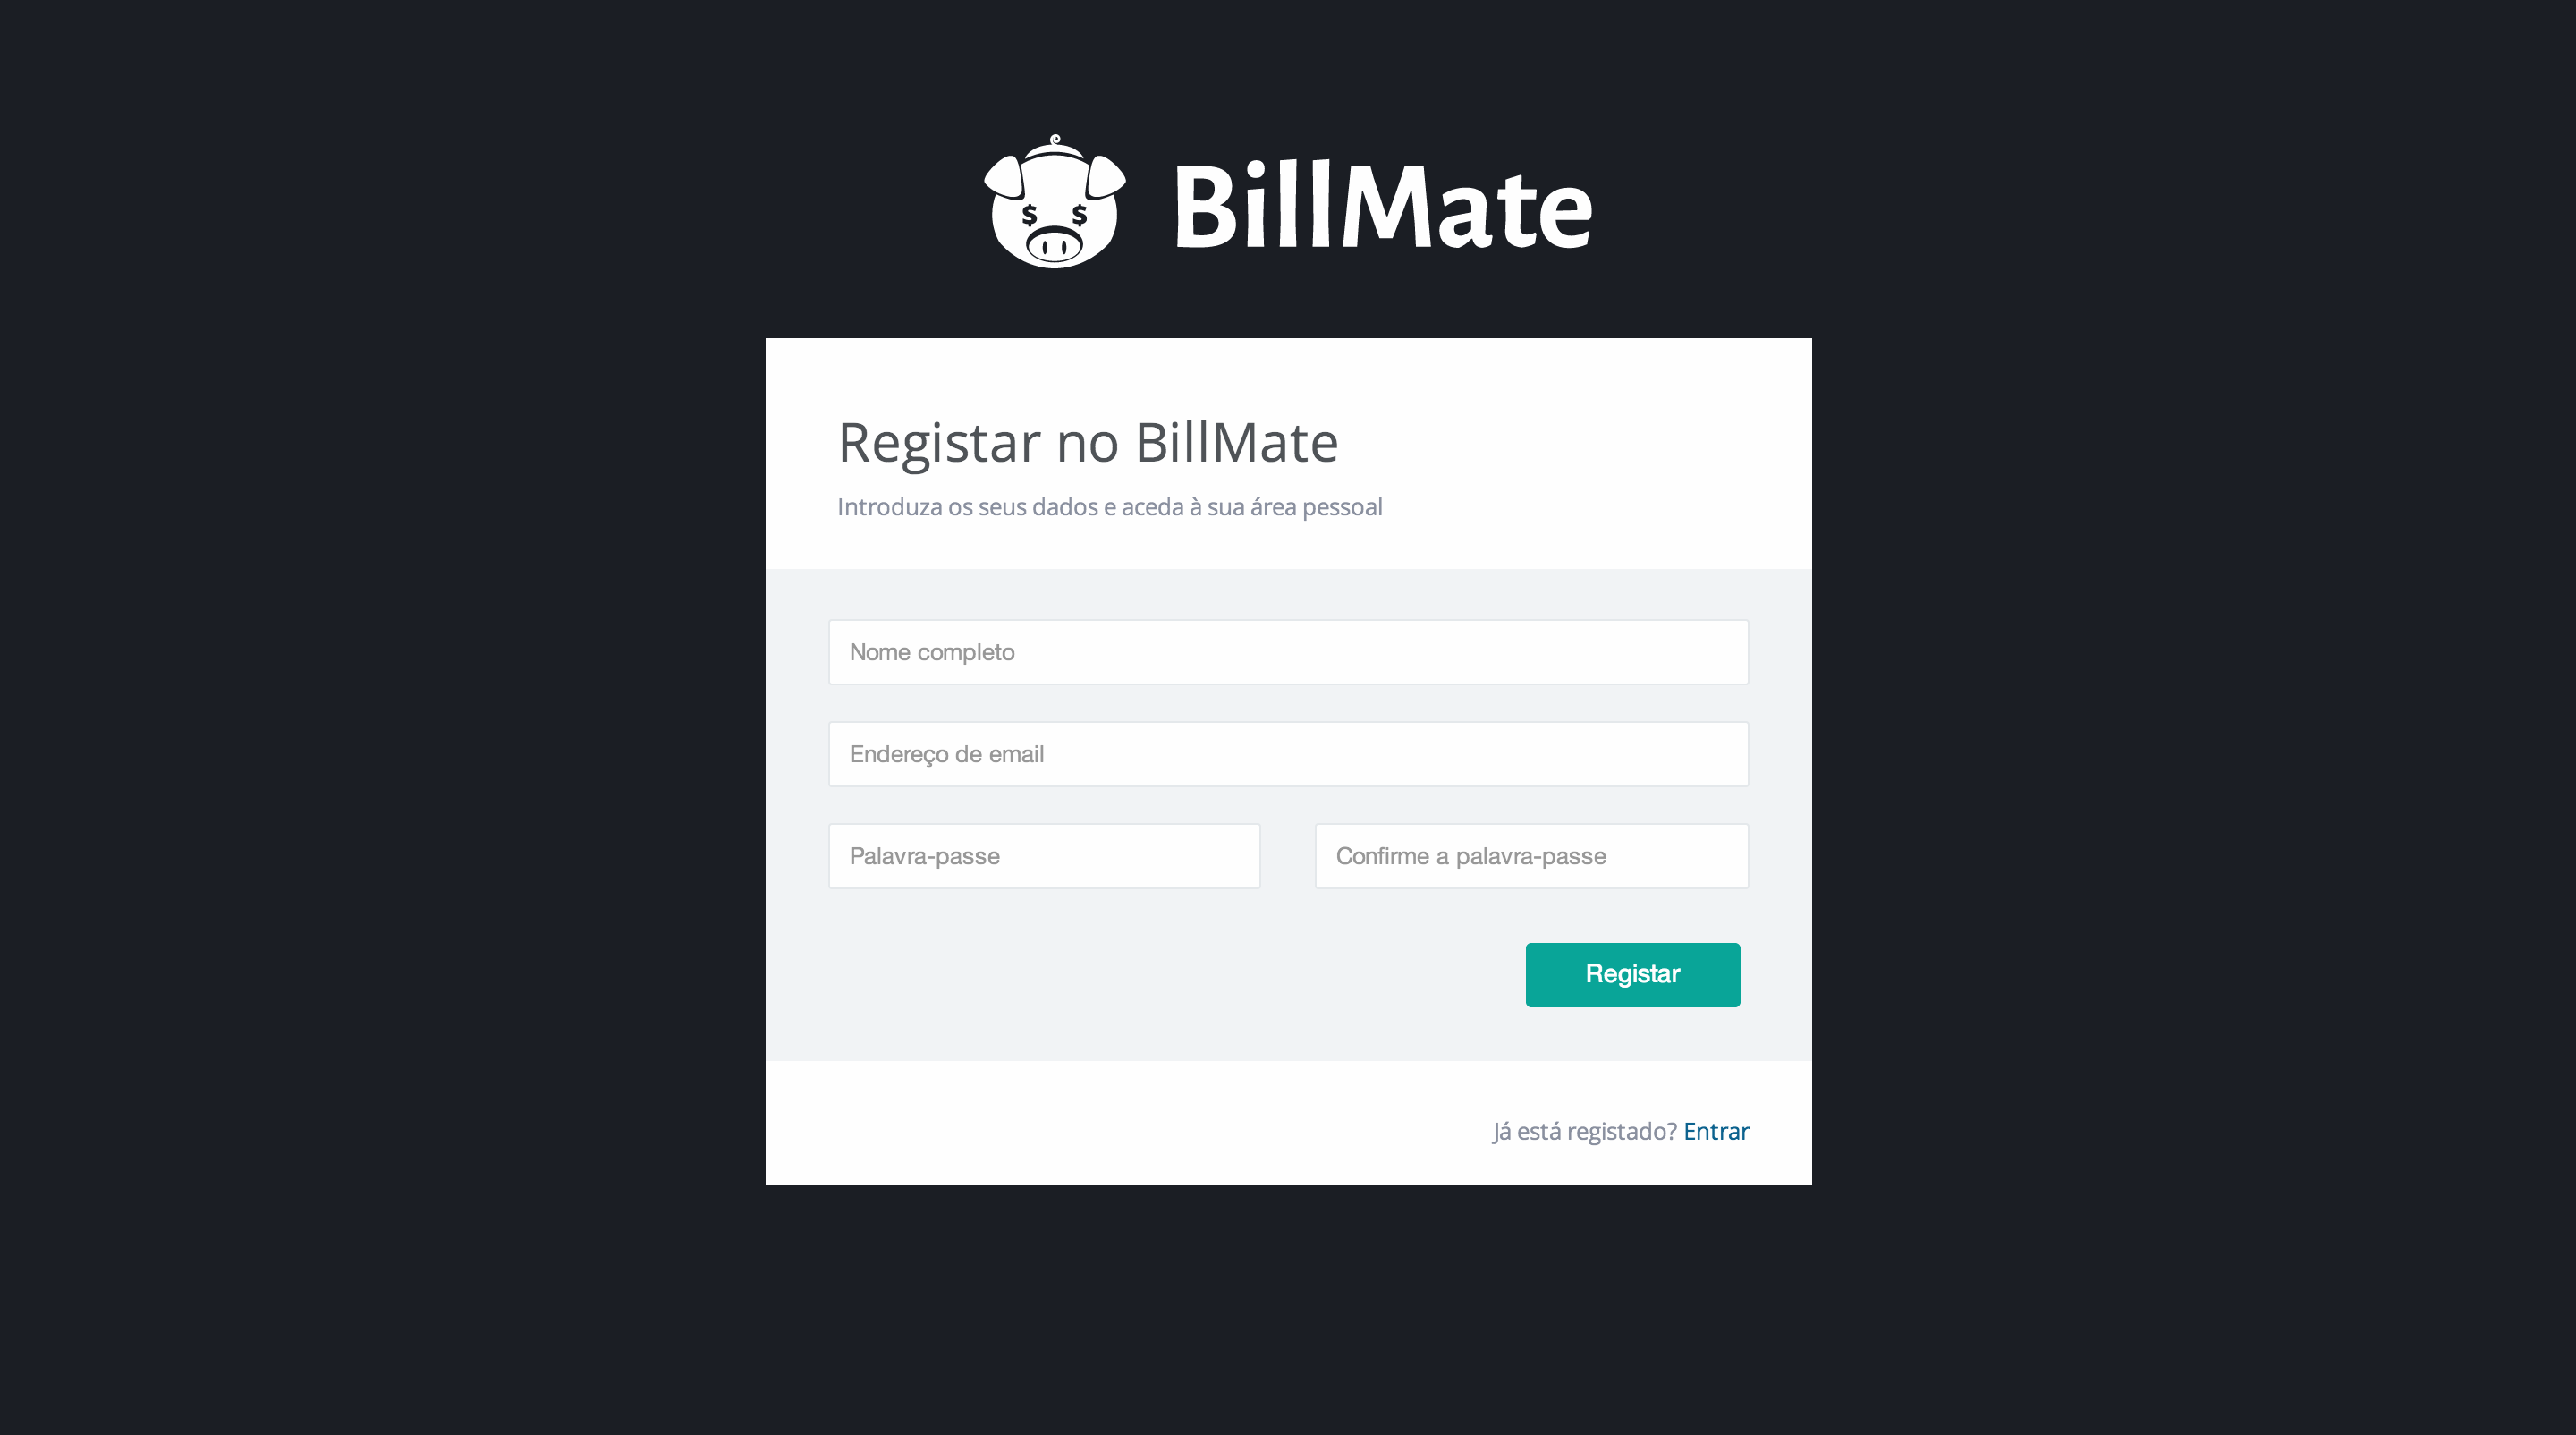
\includegraphics[width=.5\textwidth]{images/andre/registo}
\caption{Registo}
}
\end{figure}

\begin{figure}[ht]
\sidebyside{
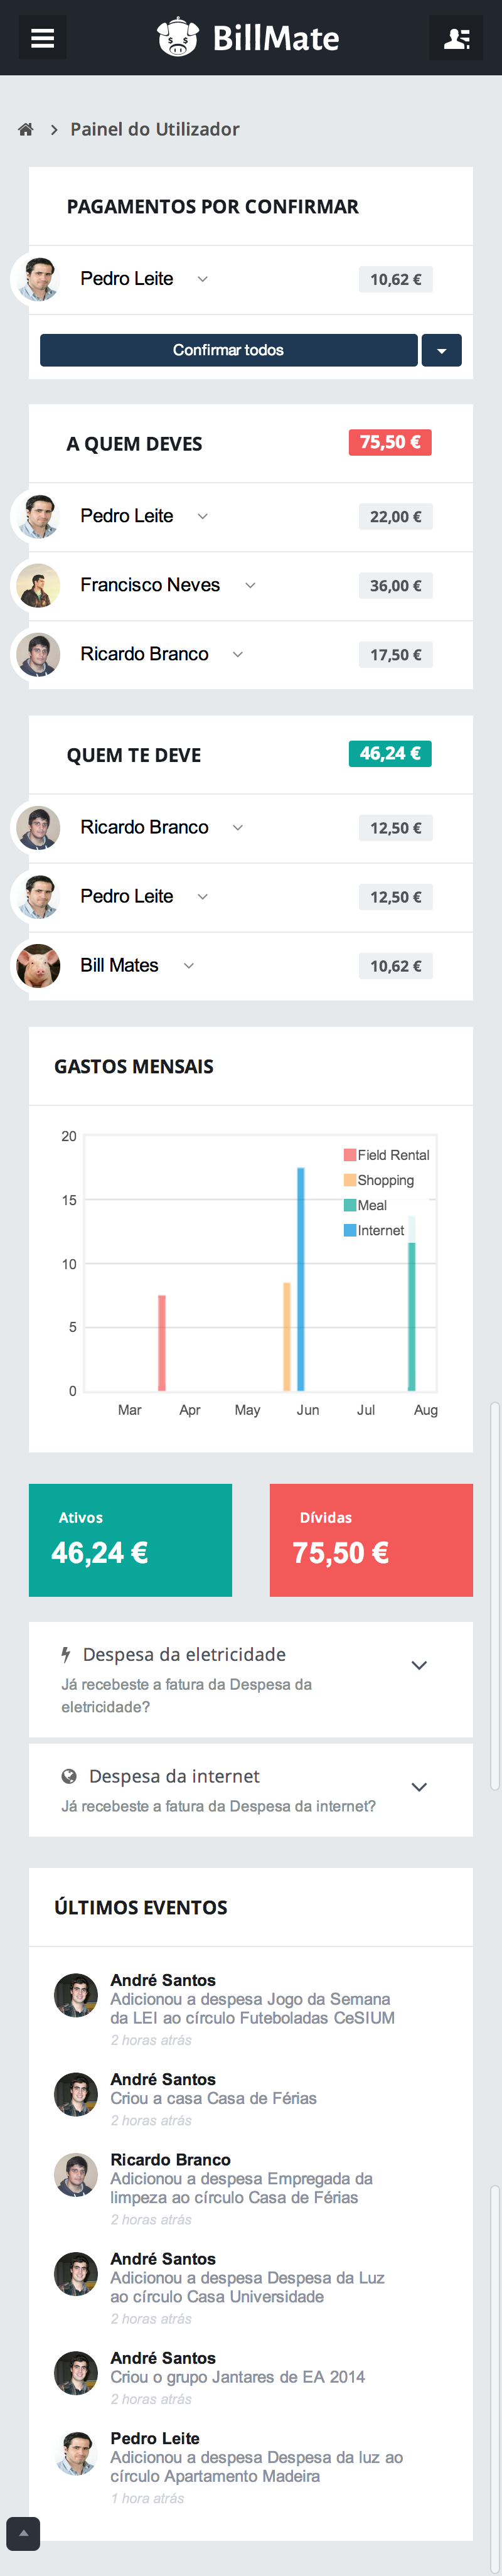
\includegraphics[width=.5\textwidth]{images/andre/dash_r}
\caption{Dashboard - Responsive}
}
{
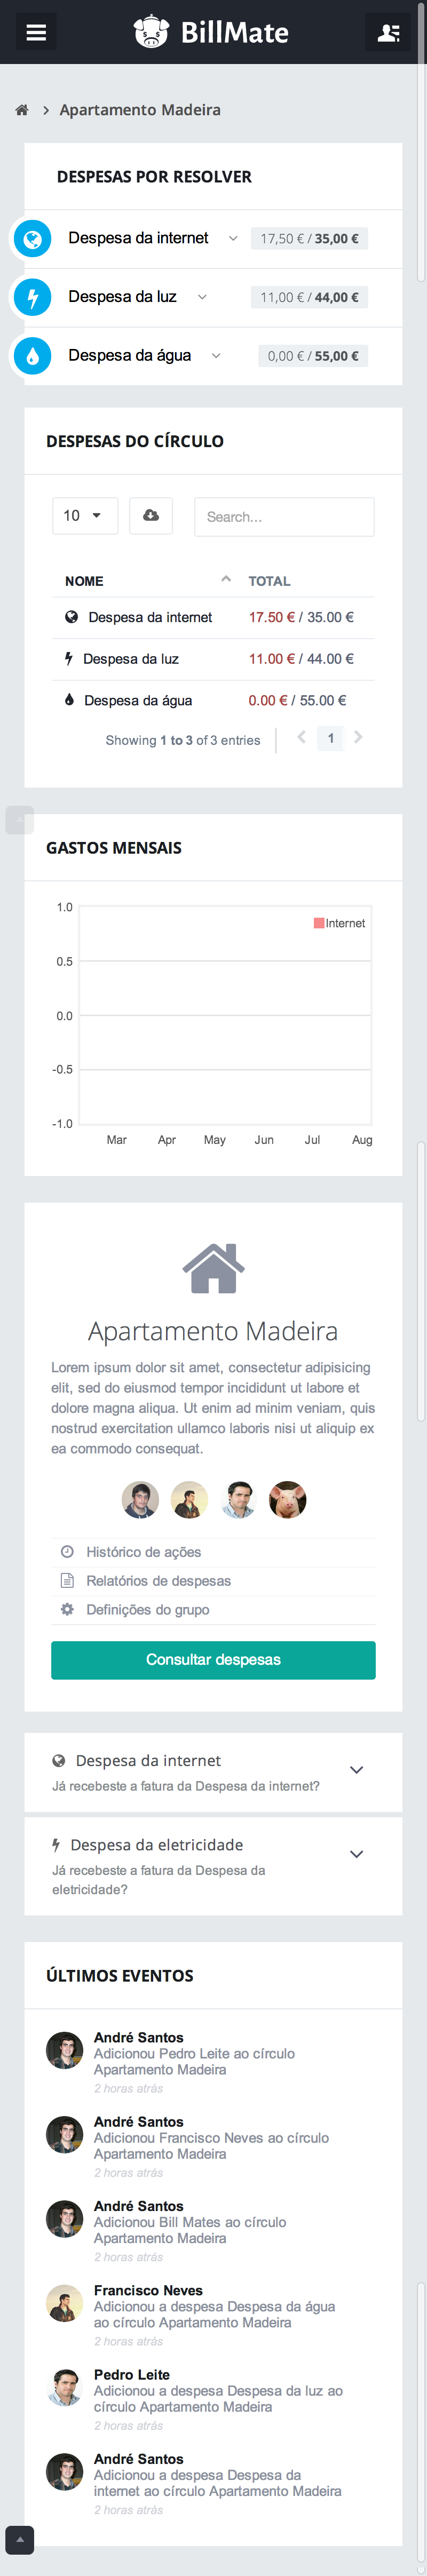
\includegraphics[width=.5\textwidth]{images/andre/circler}
\caption{Dashboard de um circulo - Responsive }
}
\end{figure}

\begin{figure}[ht]
\sidebyside{
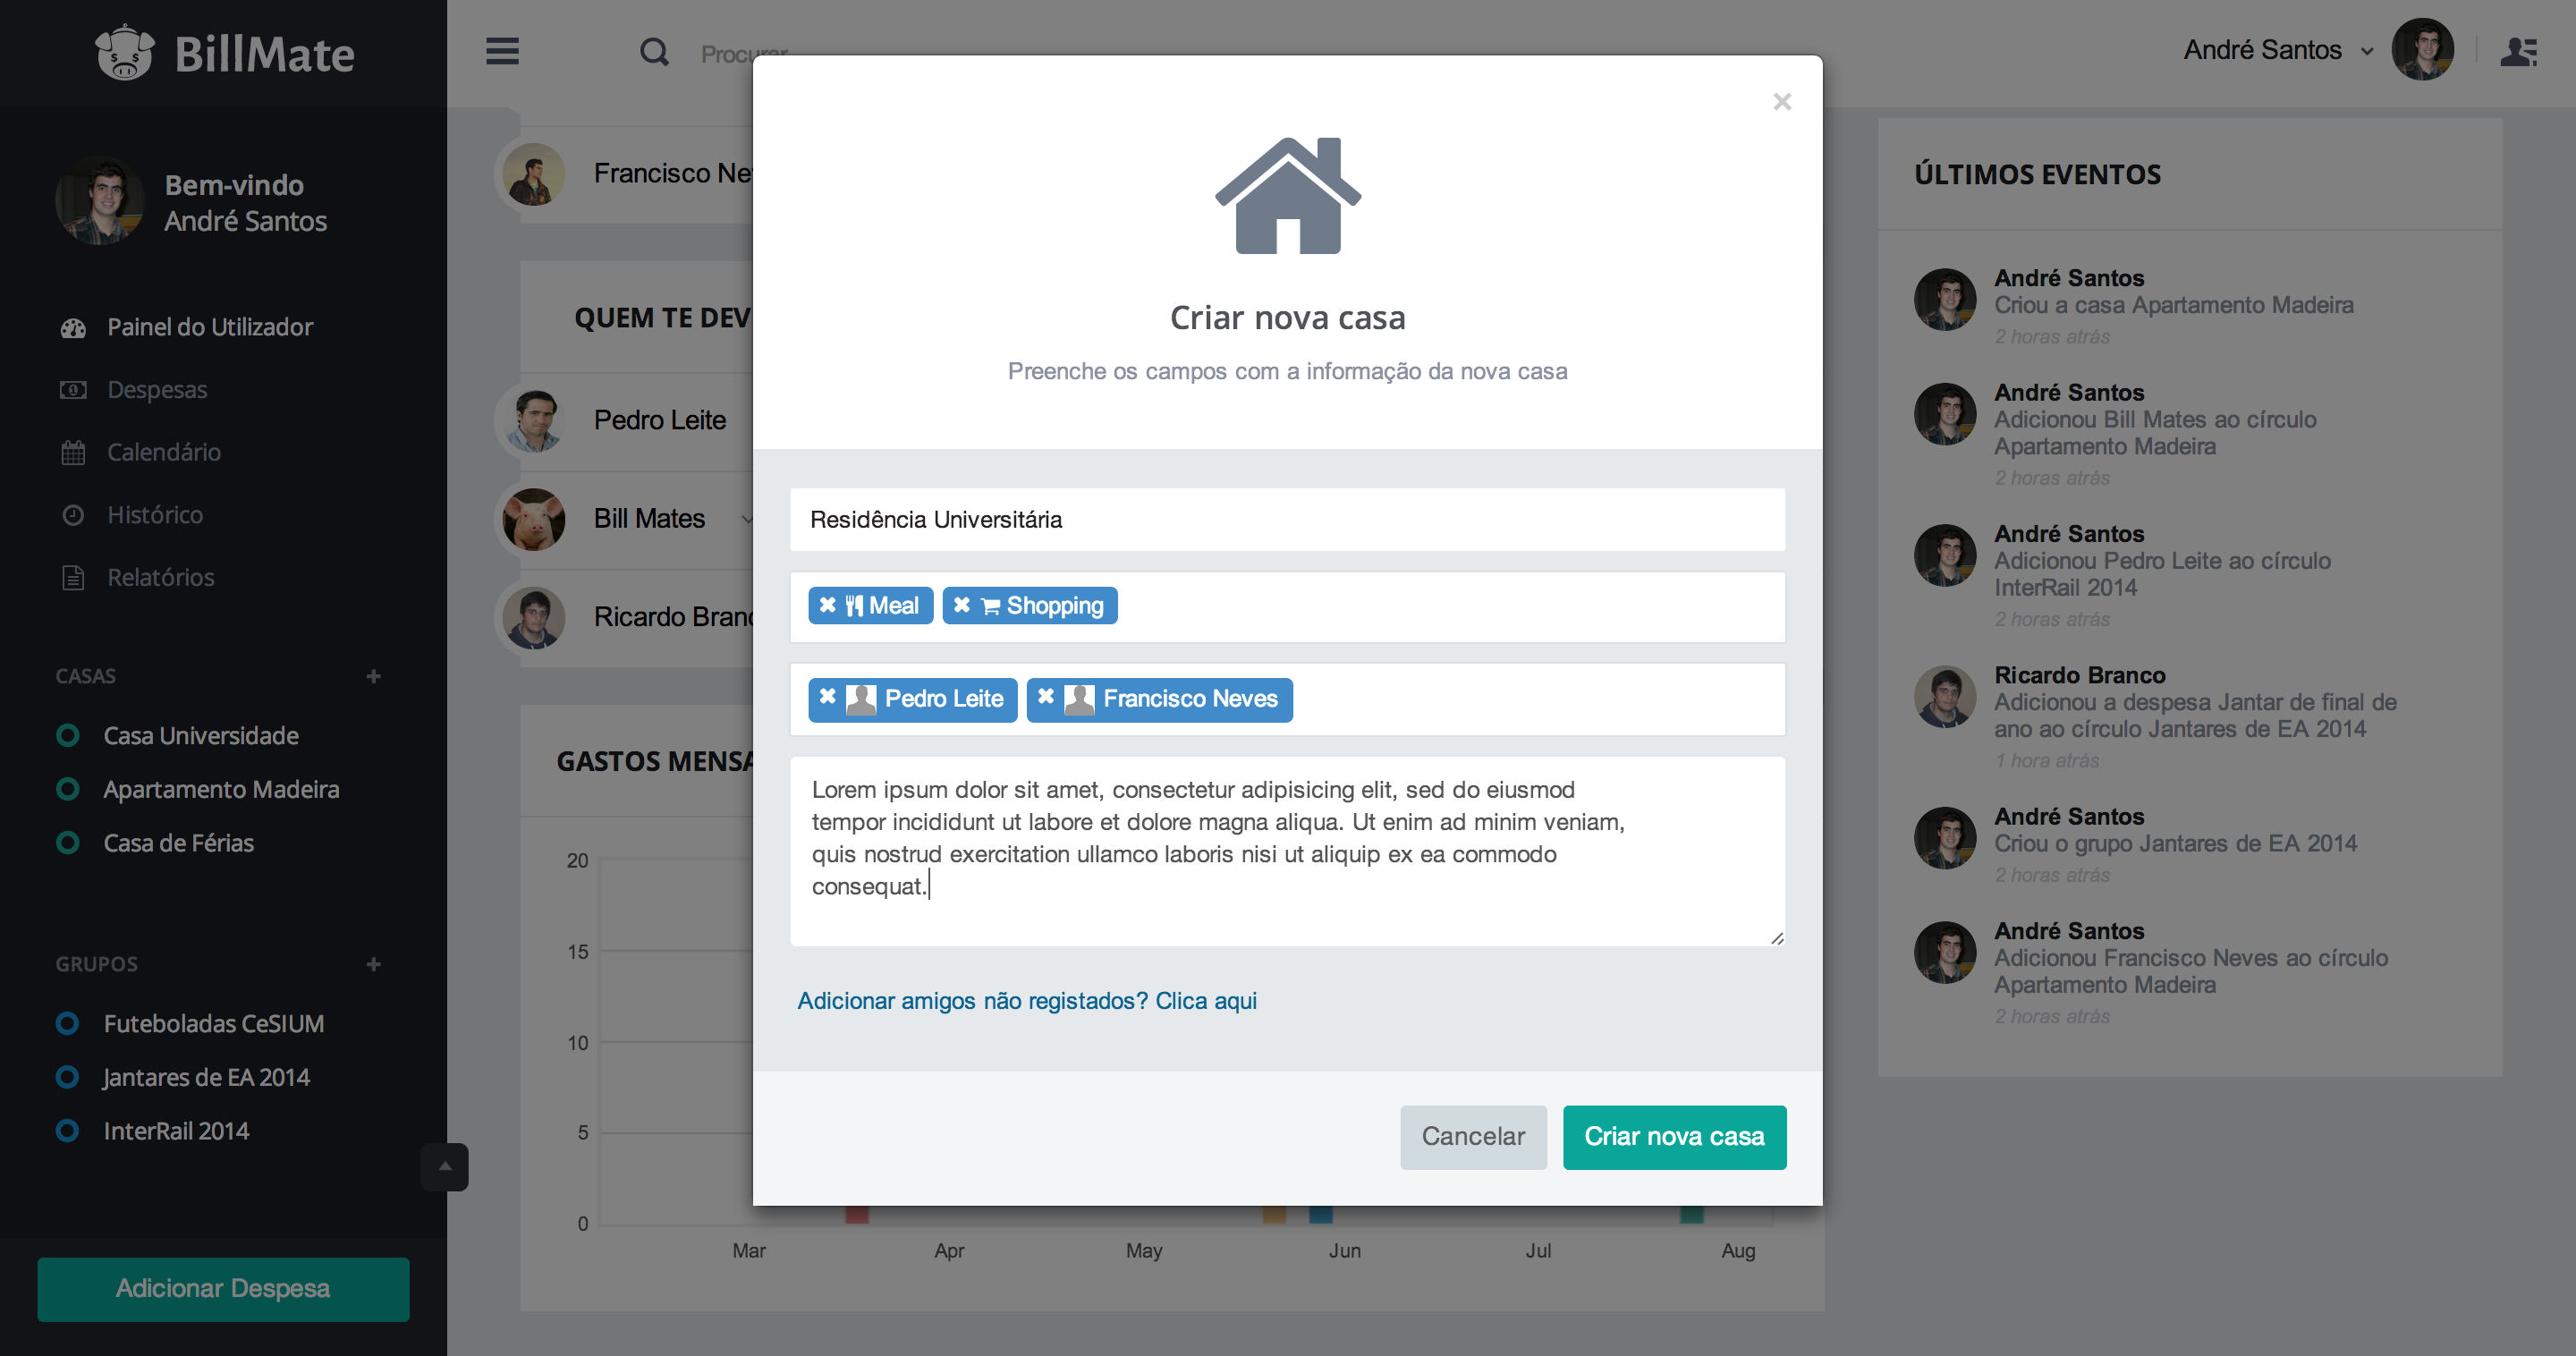
\includegraphics[width=.5\textwidth]{images/andre/create_house}
\caption{Criar Casa}
}
{
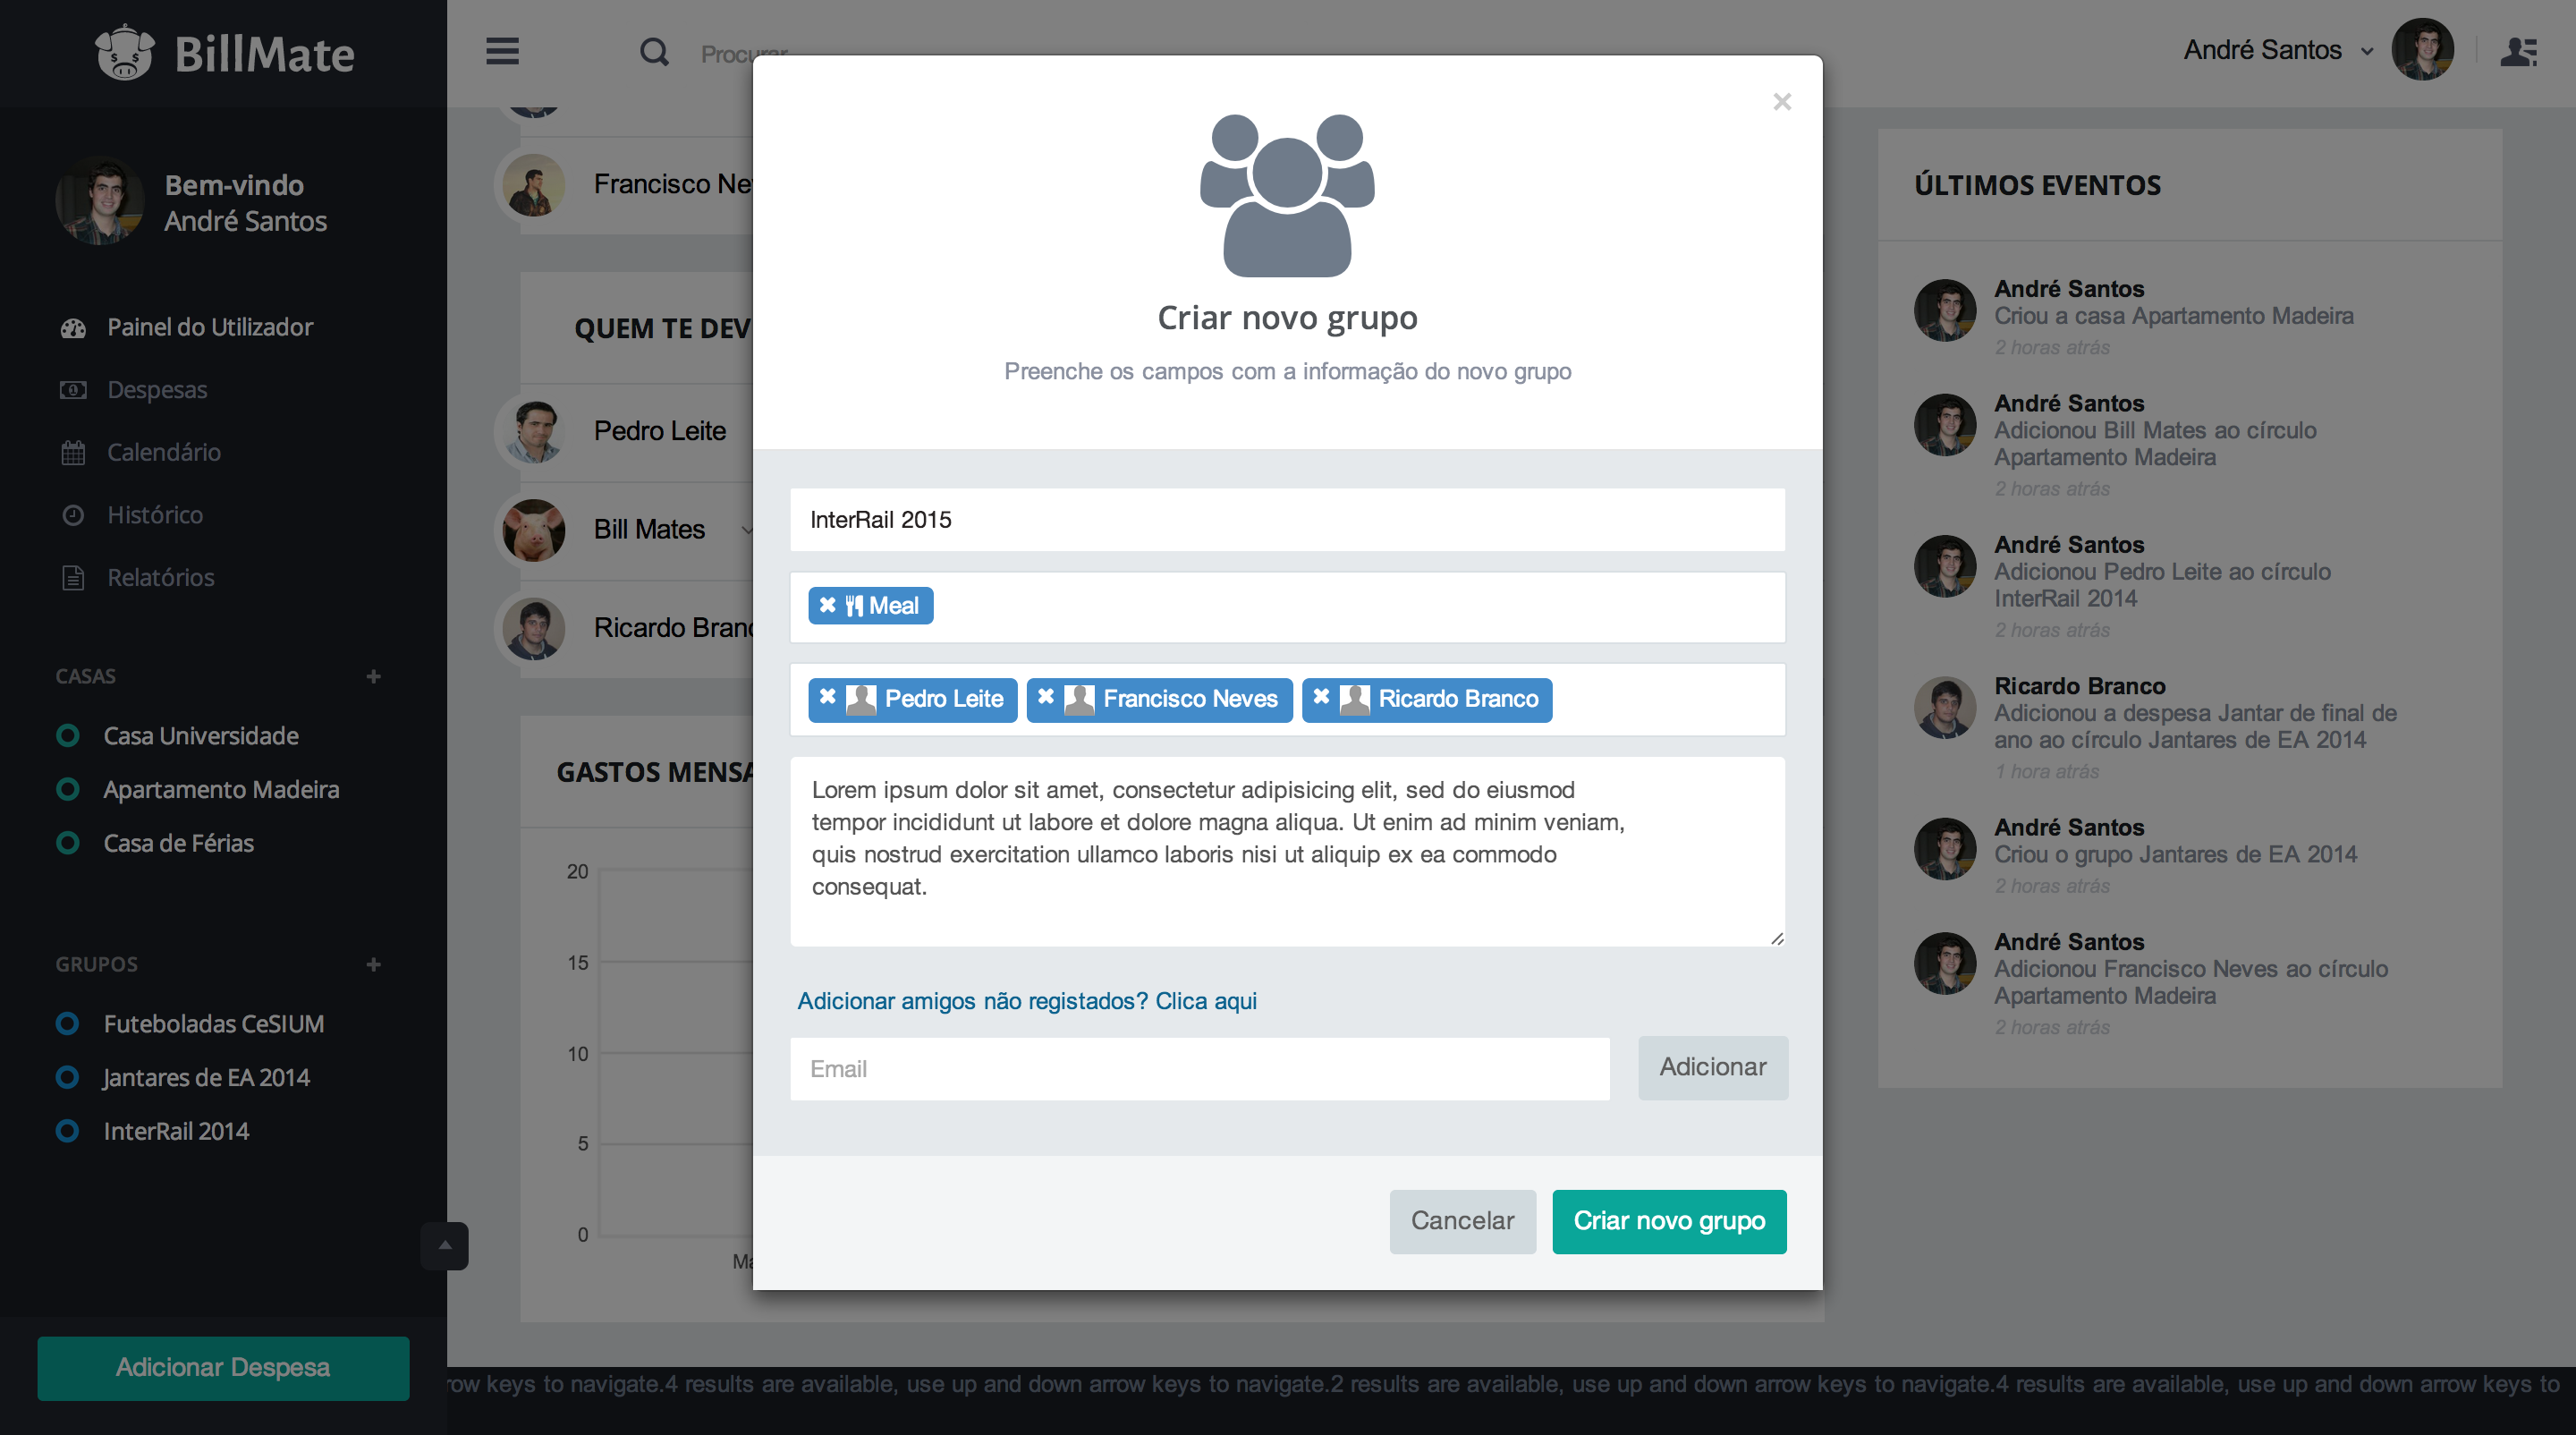
\includegraphics[width=.5\textwidth]{images/andre/create_collective}
\caption{Criar Grupo}
}
\end{figure}

\begin{figure}[ht]
\sidebyside{
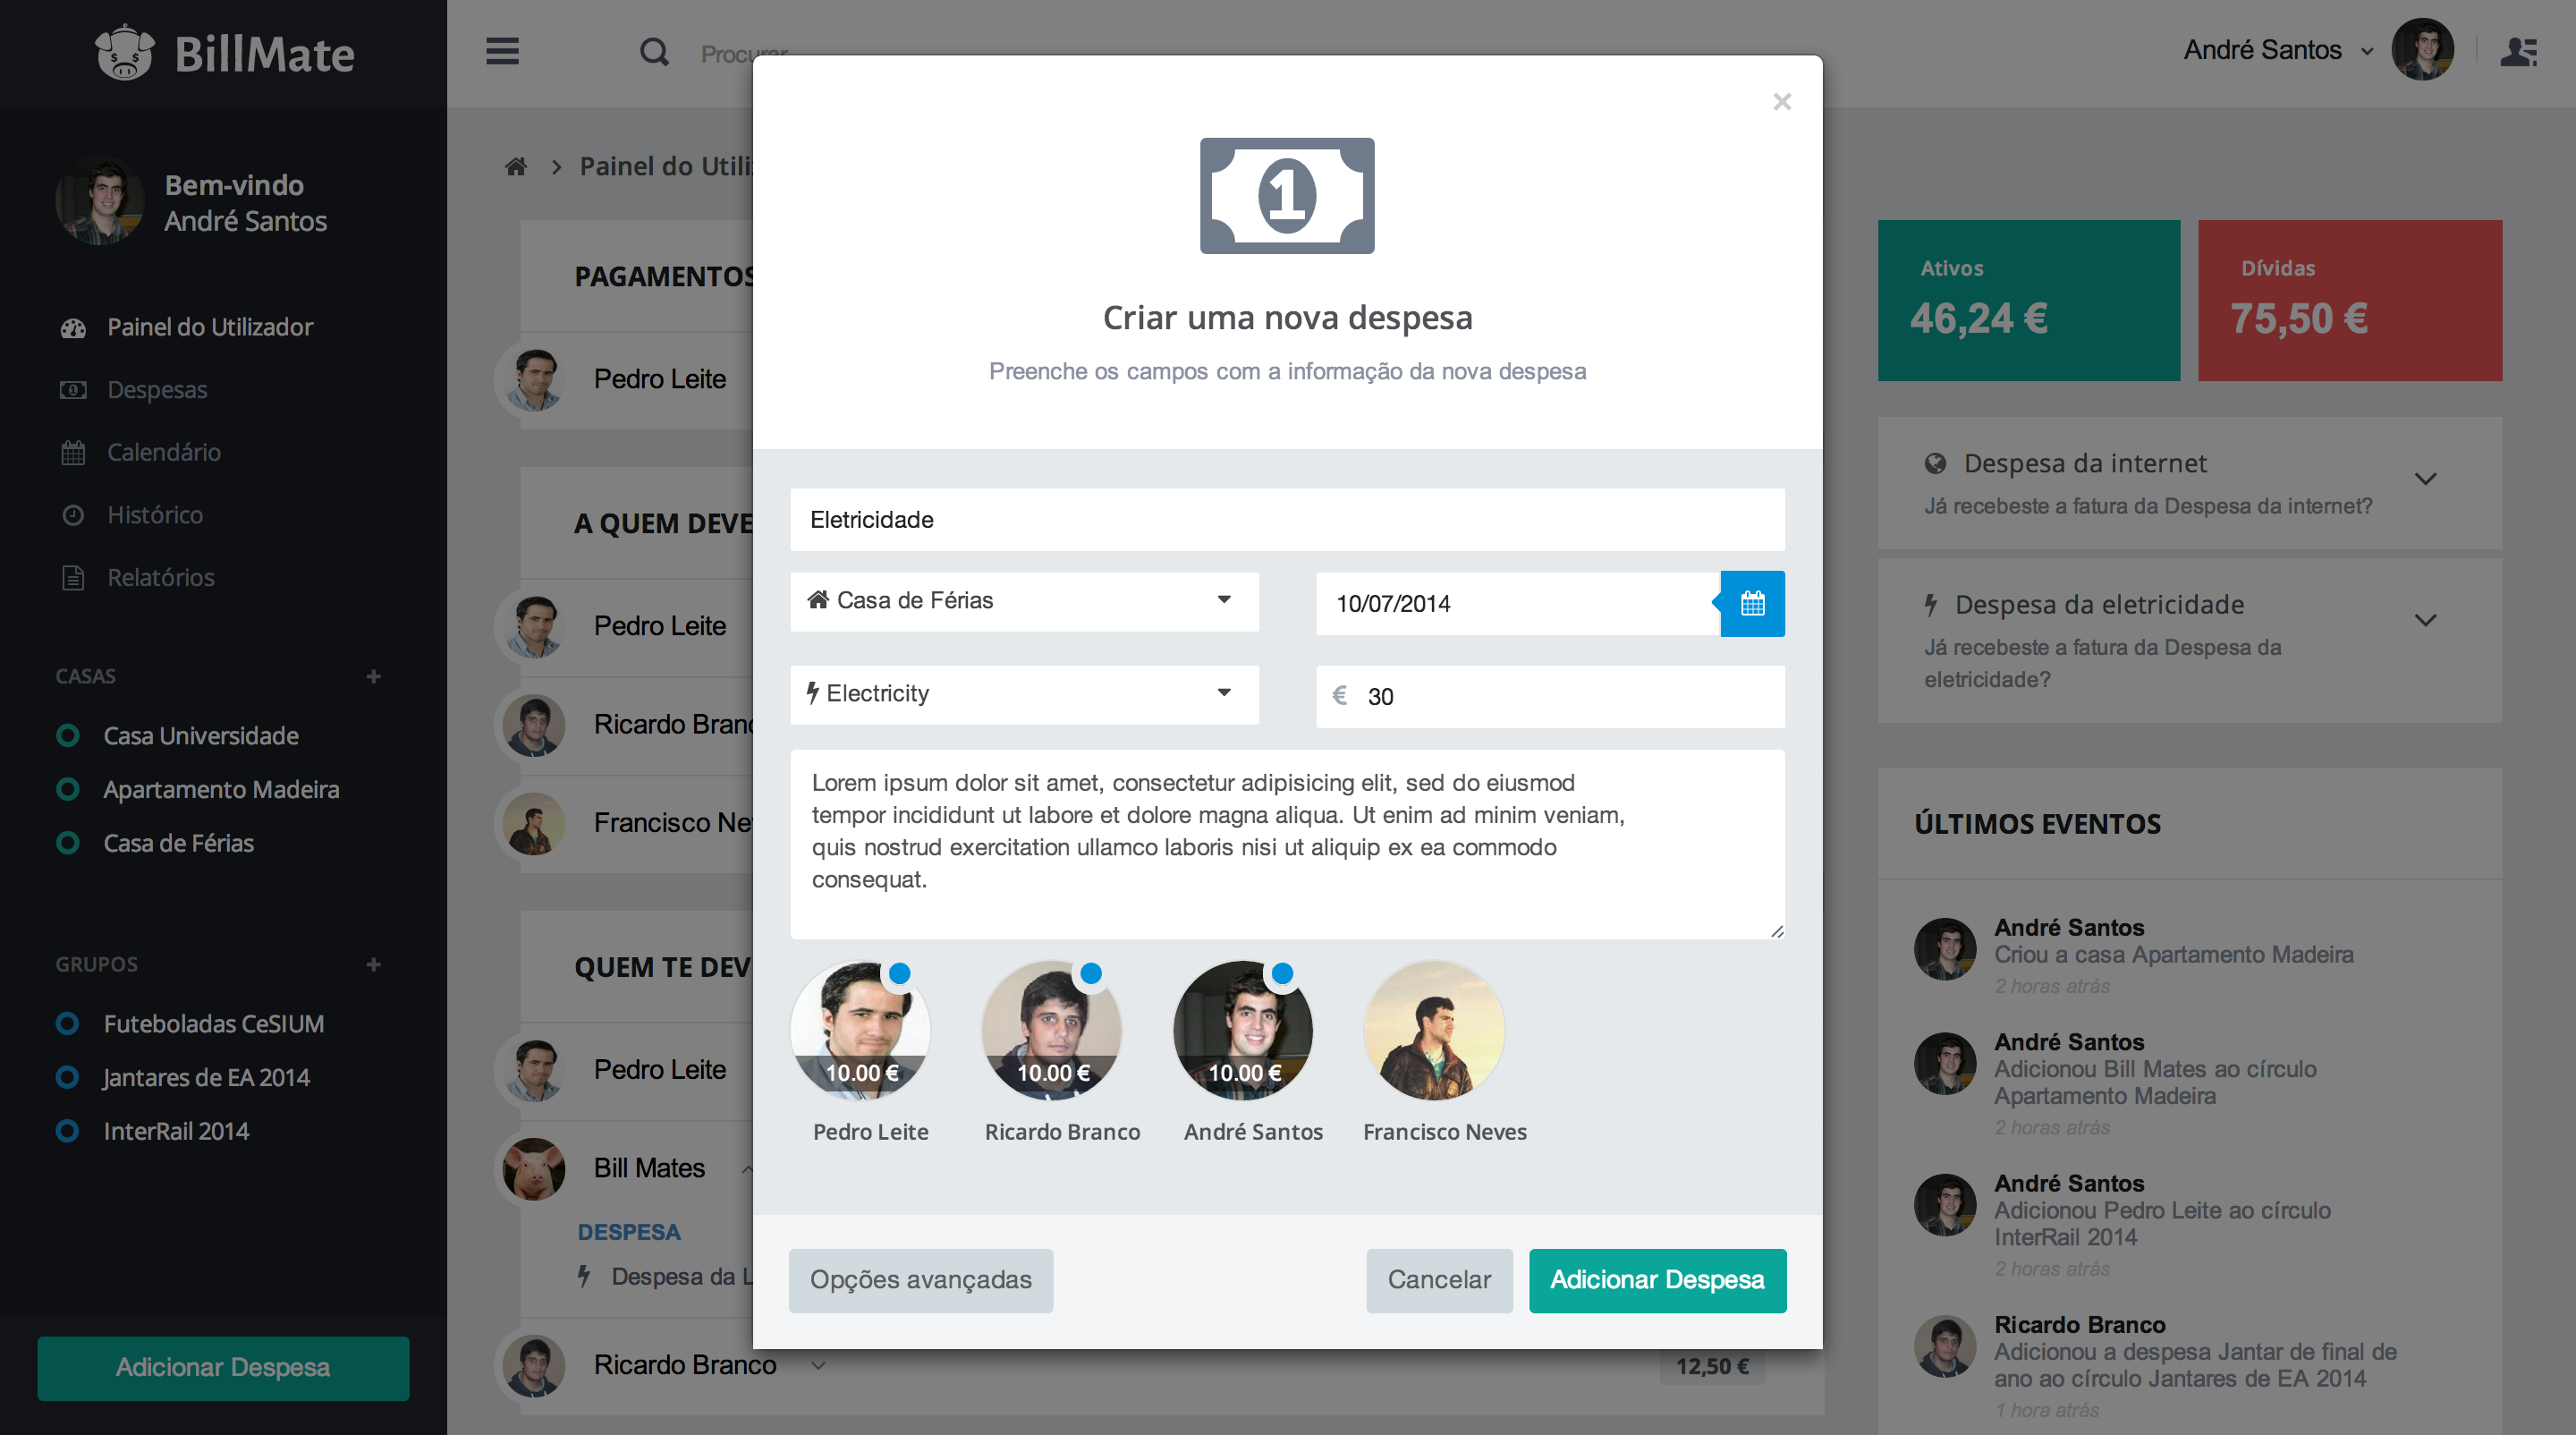
\includegraphics[width=.5\textwidth]{images/andre/create_expense}
\caption{Criar despesa}
}
{
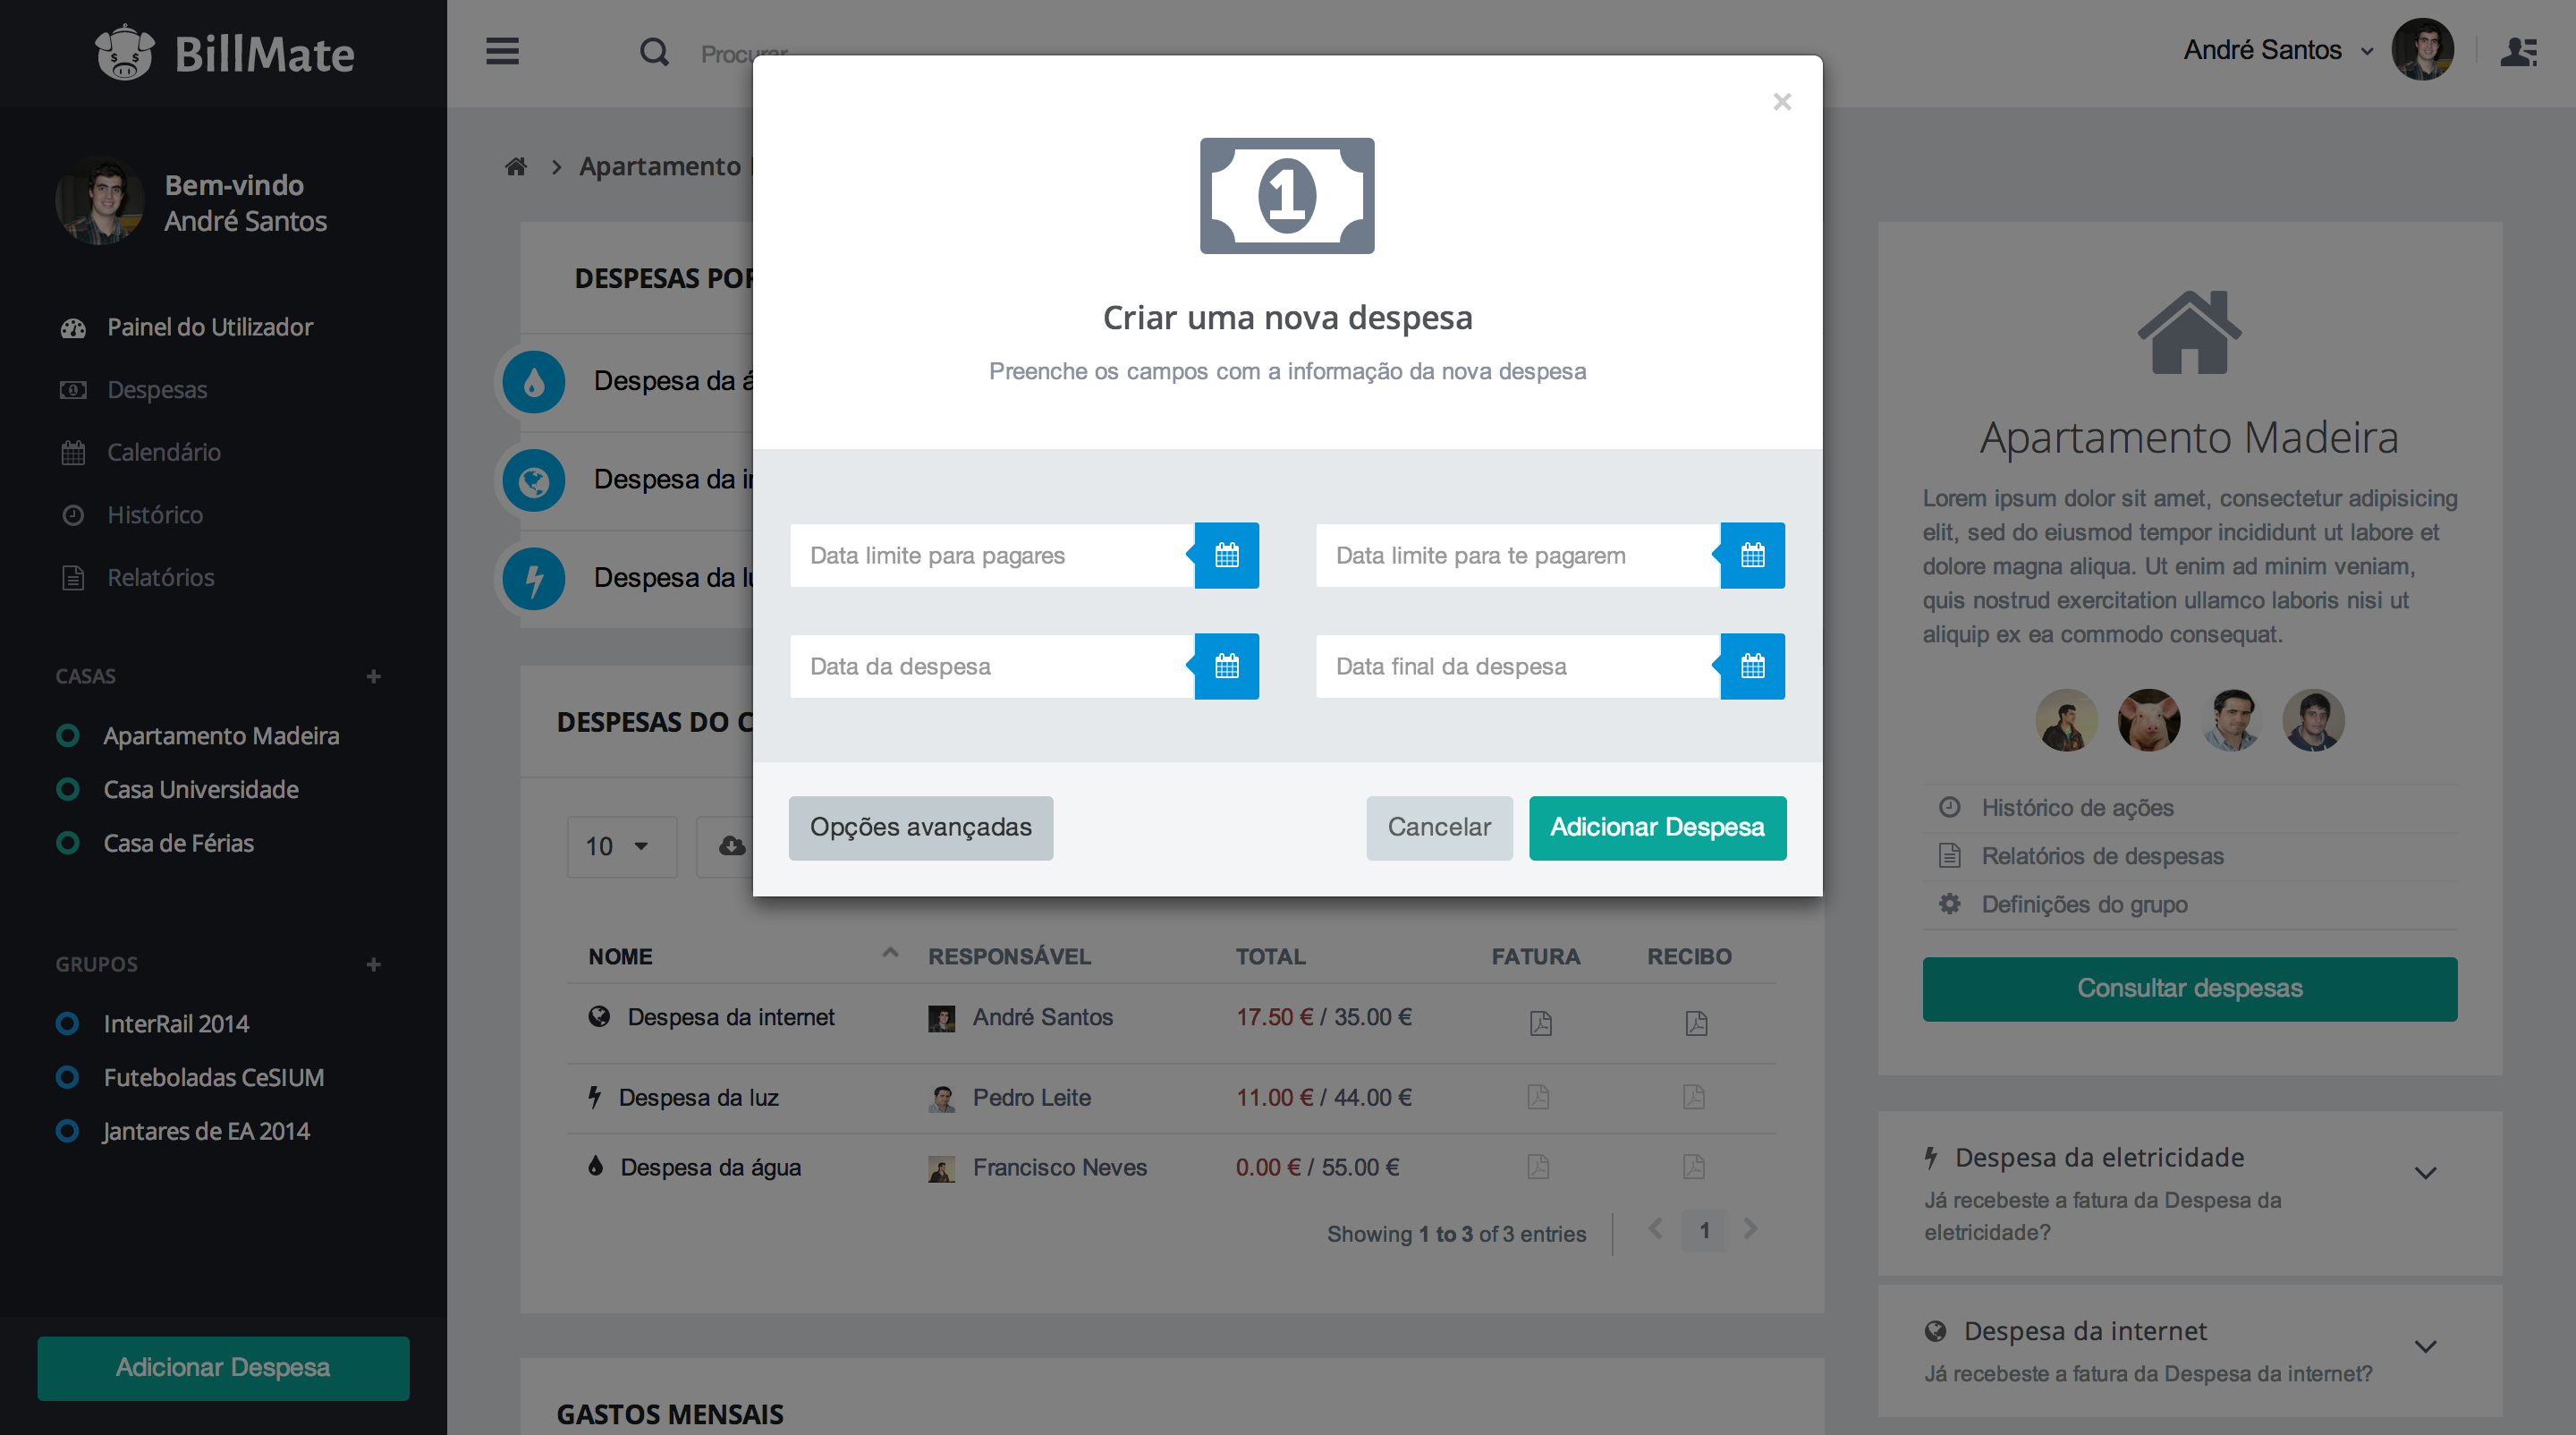
\includegraphics[width=.5\textwidth]{images/andre/cexpadv}
\caption{Criar despesa - Opções Avançadas}
}
\end{figure}

\begin{figure}[ht]
\sidebyside{
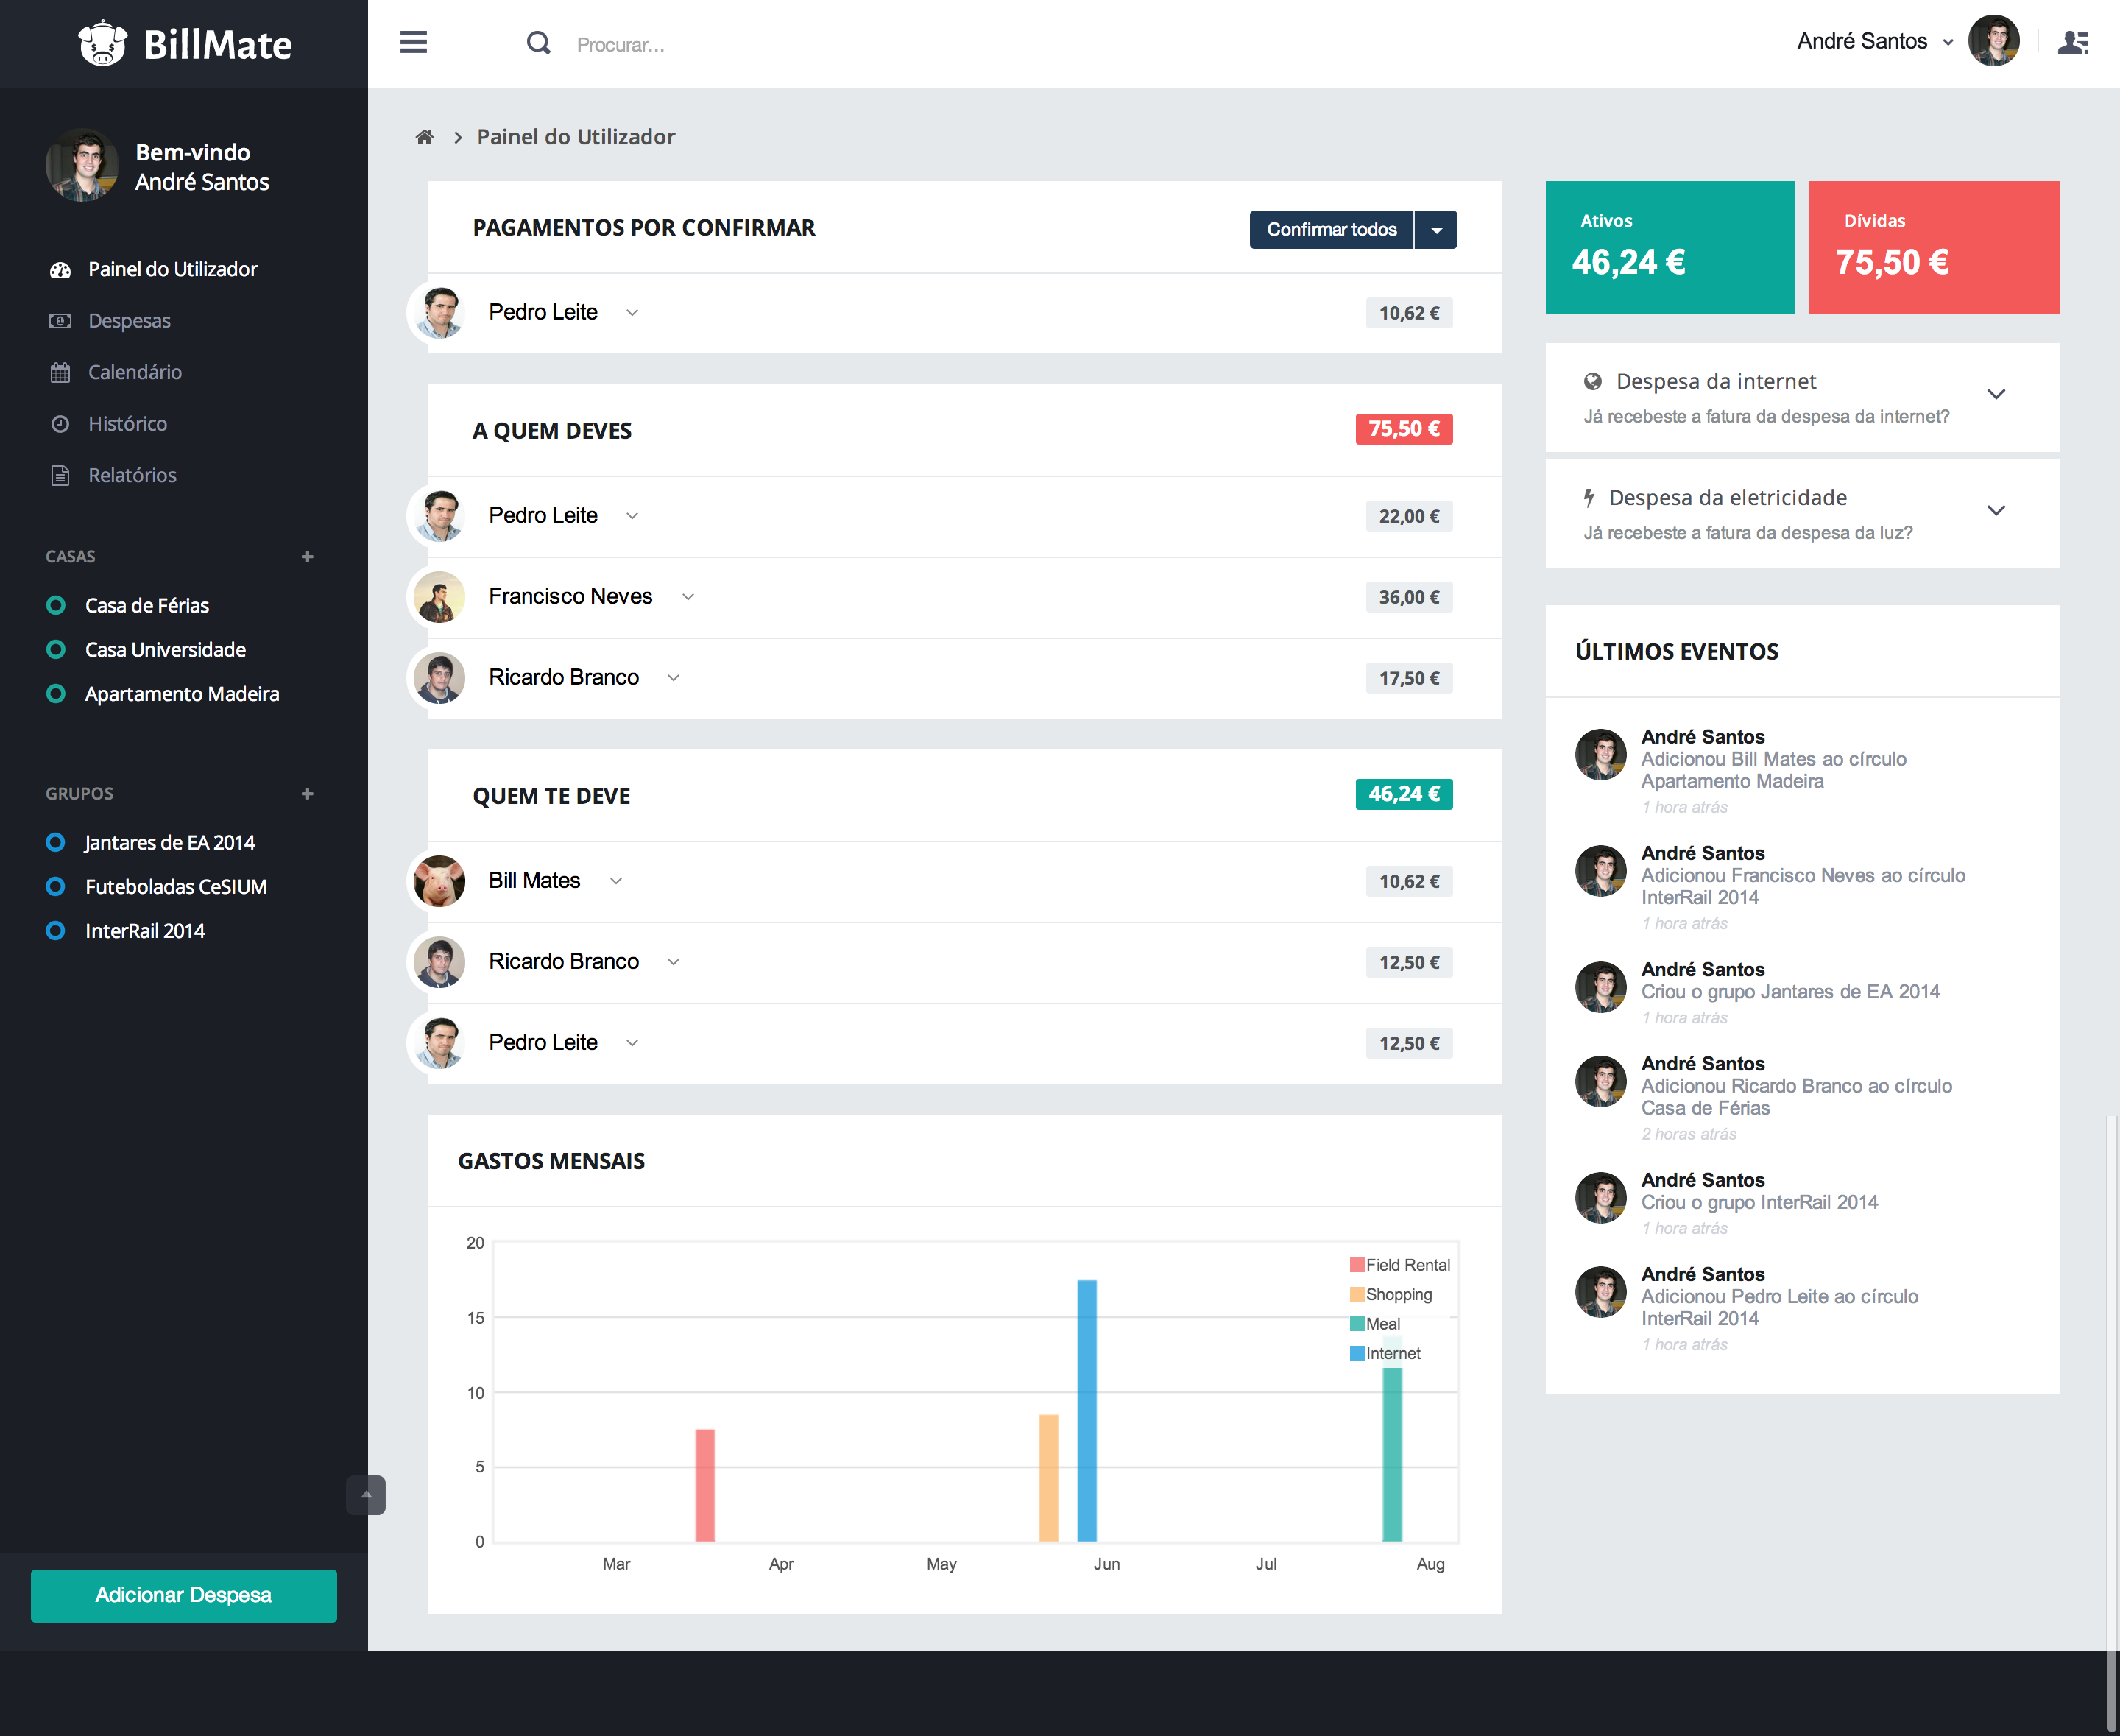
\includegraphics[width=.5\textwidth]{images/andre/dashboard_user}
\caption{Dashboard do utilizador}
}
{
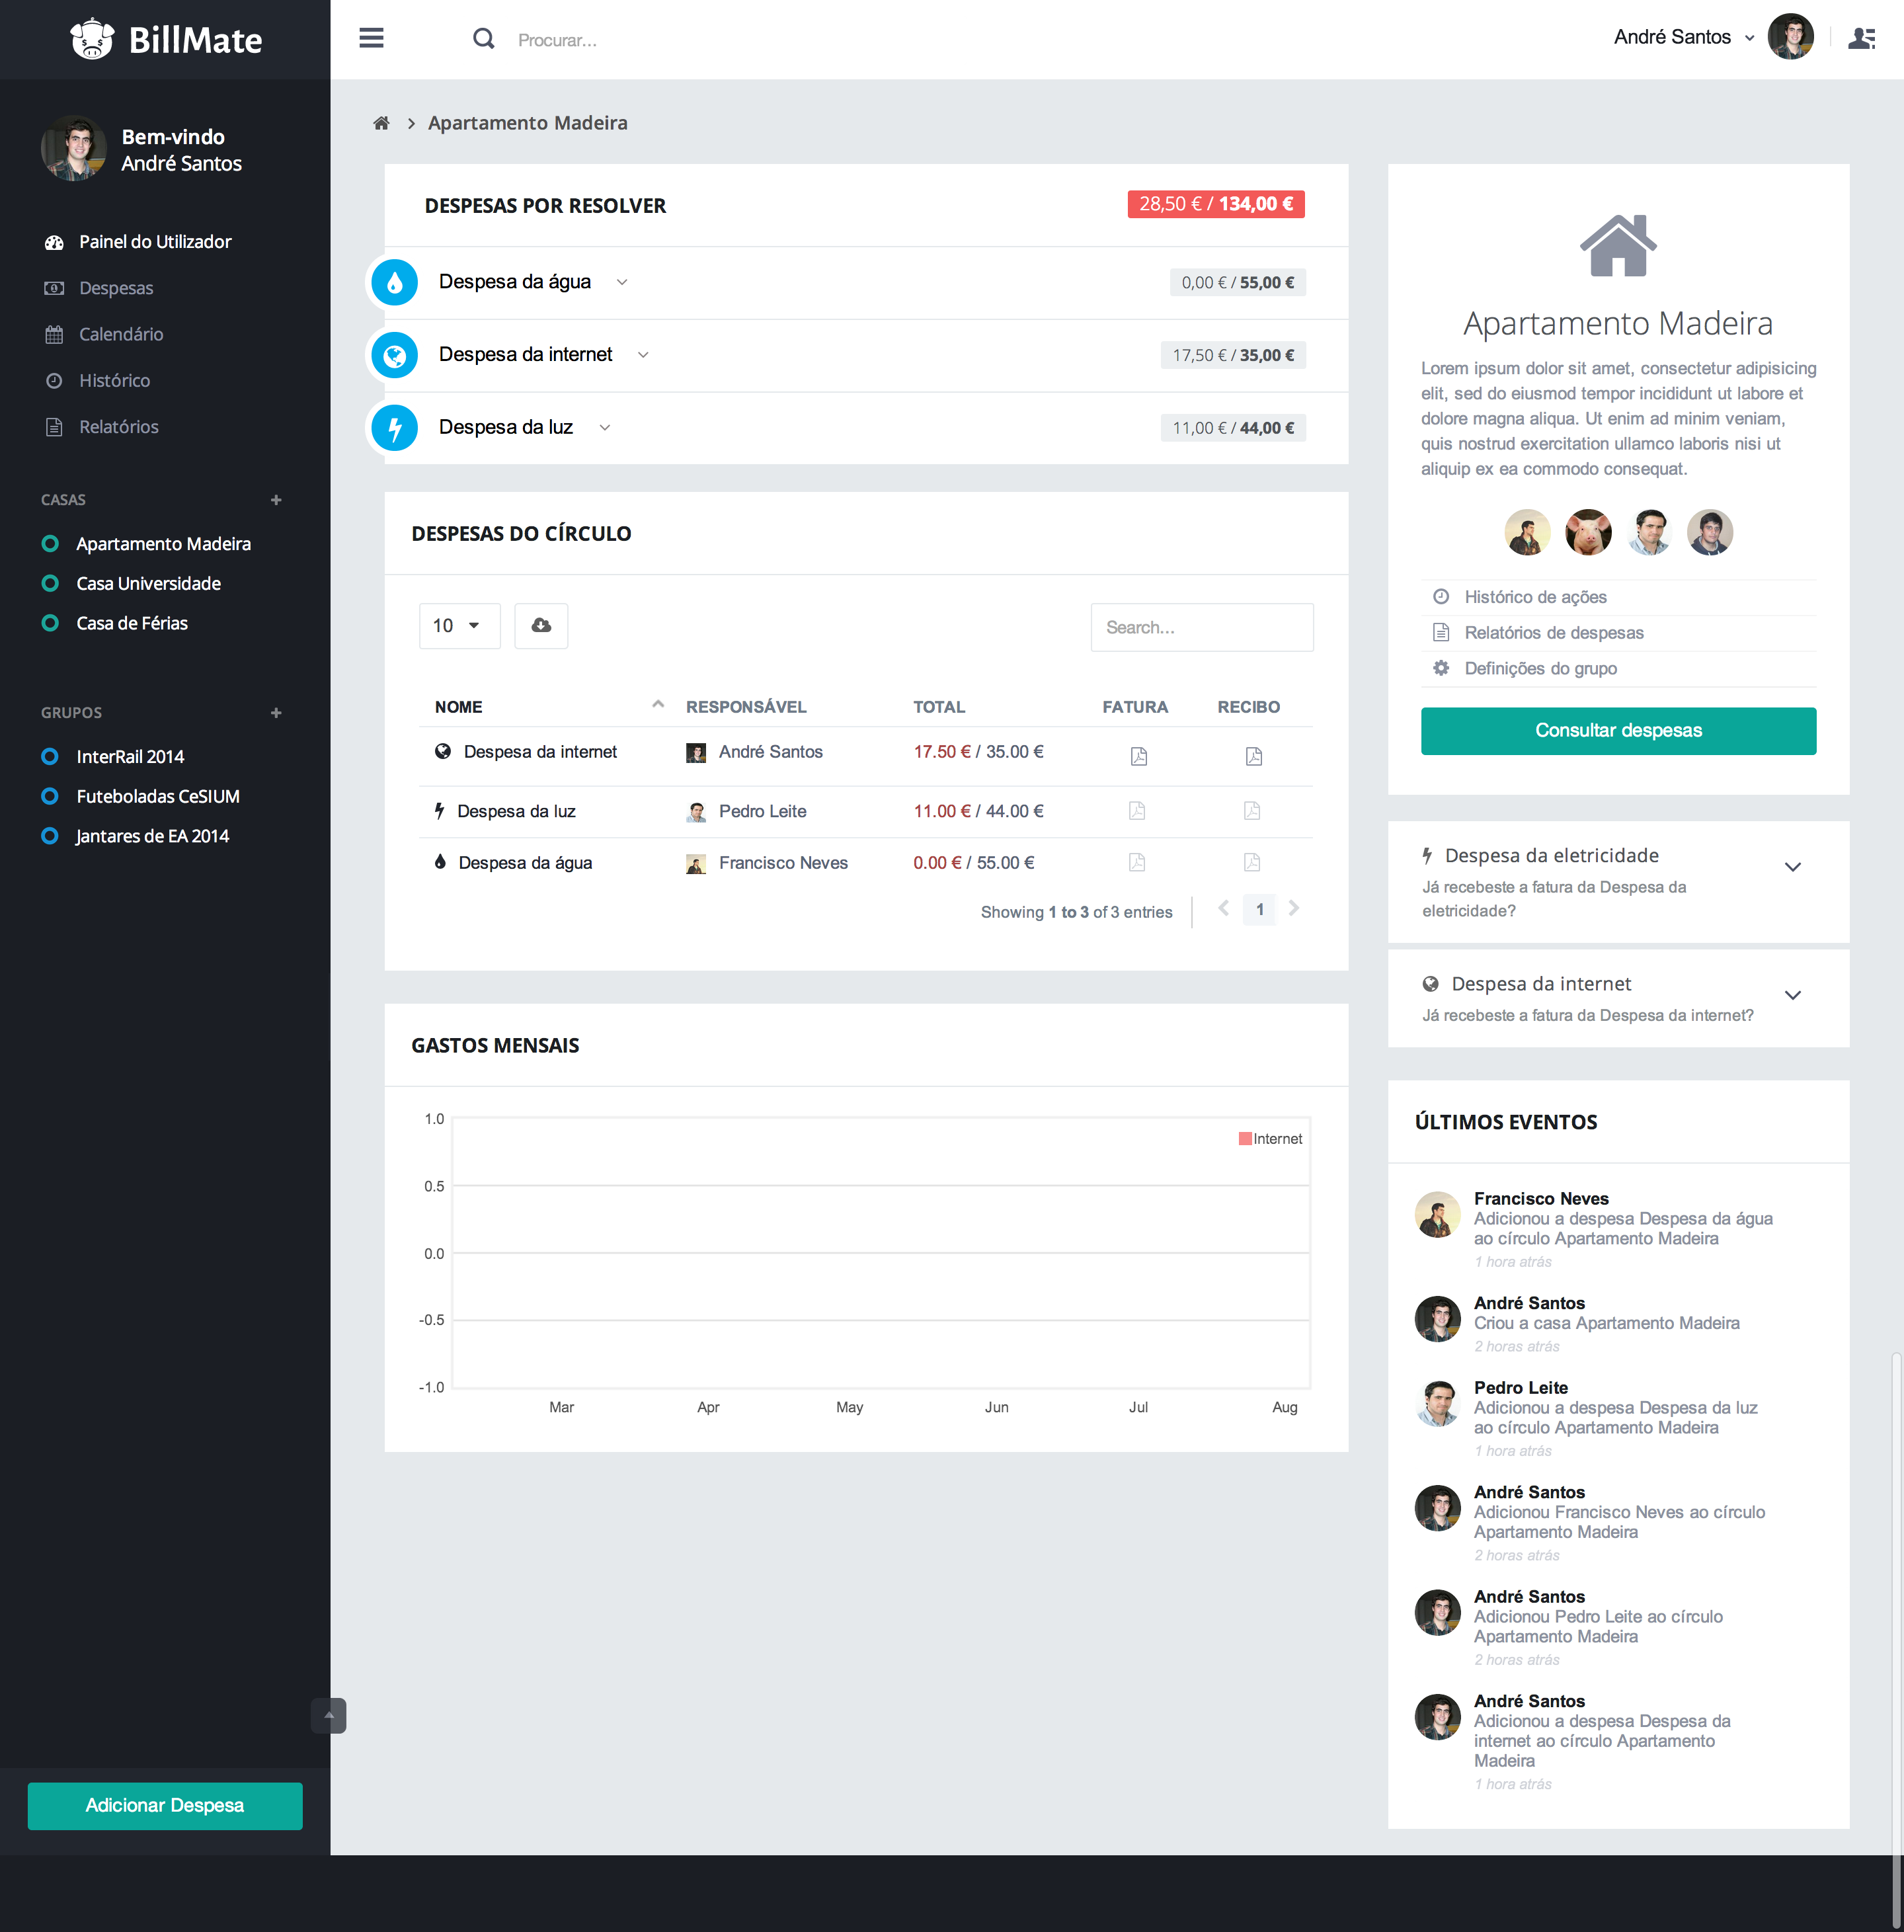
\includegraphics[width=.5\textwidth]{images/andre/dashboard_circle}
\caption{Dashboard do circulo}
}
\end{figure}

\begin{figure}[ht]
\sidebyside{
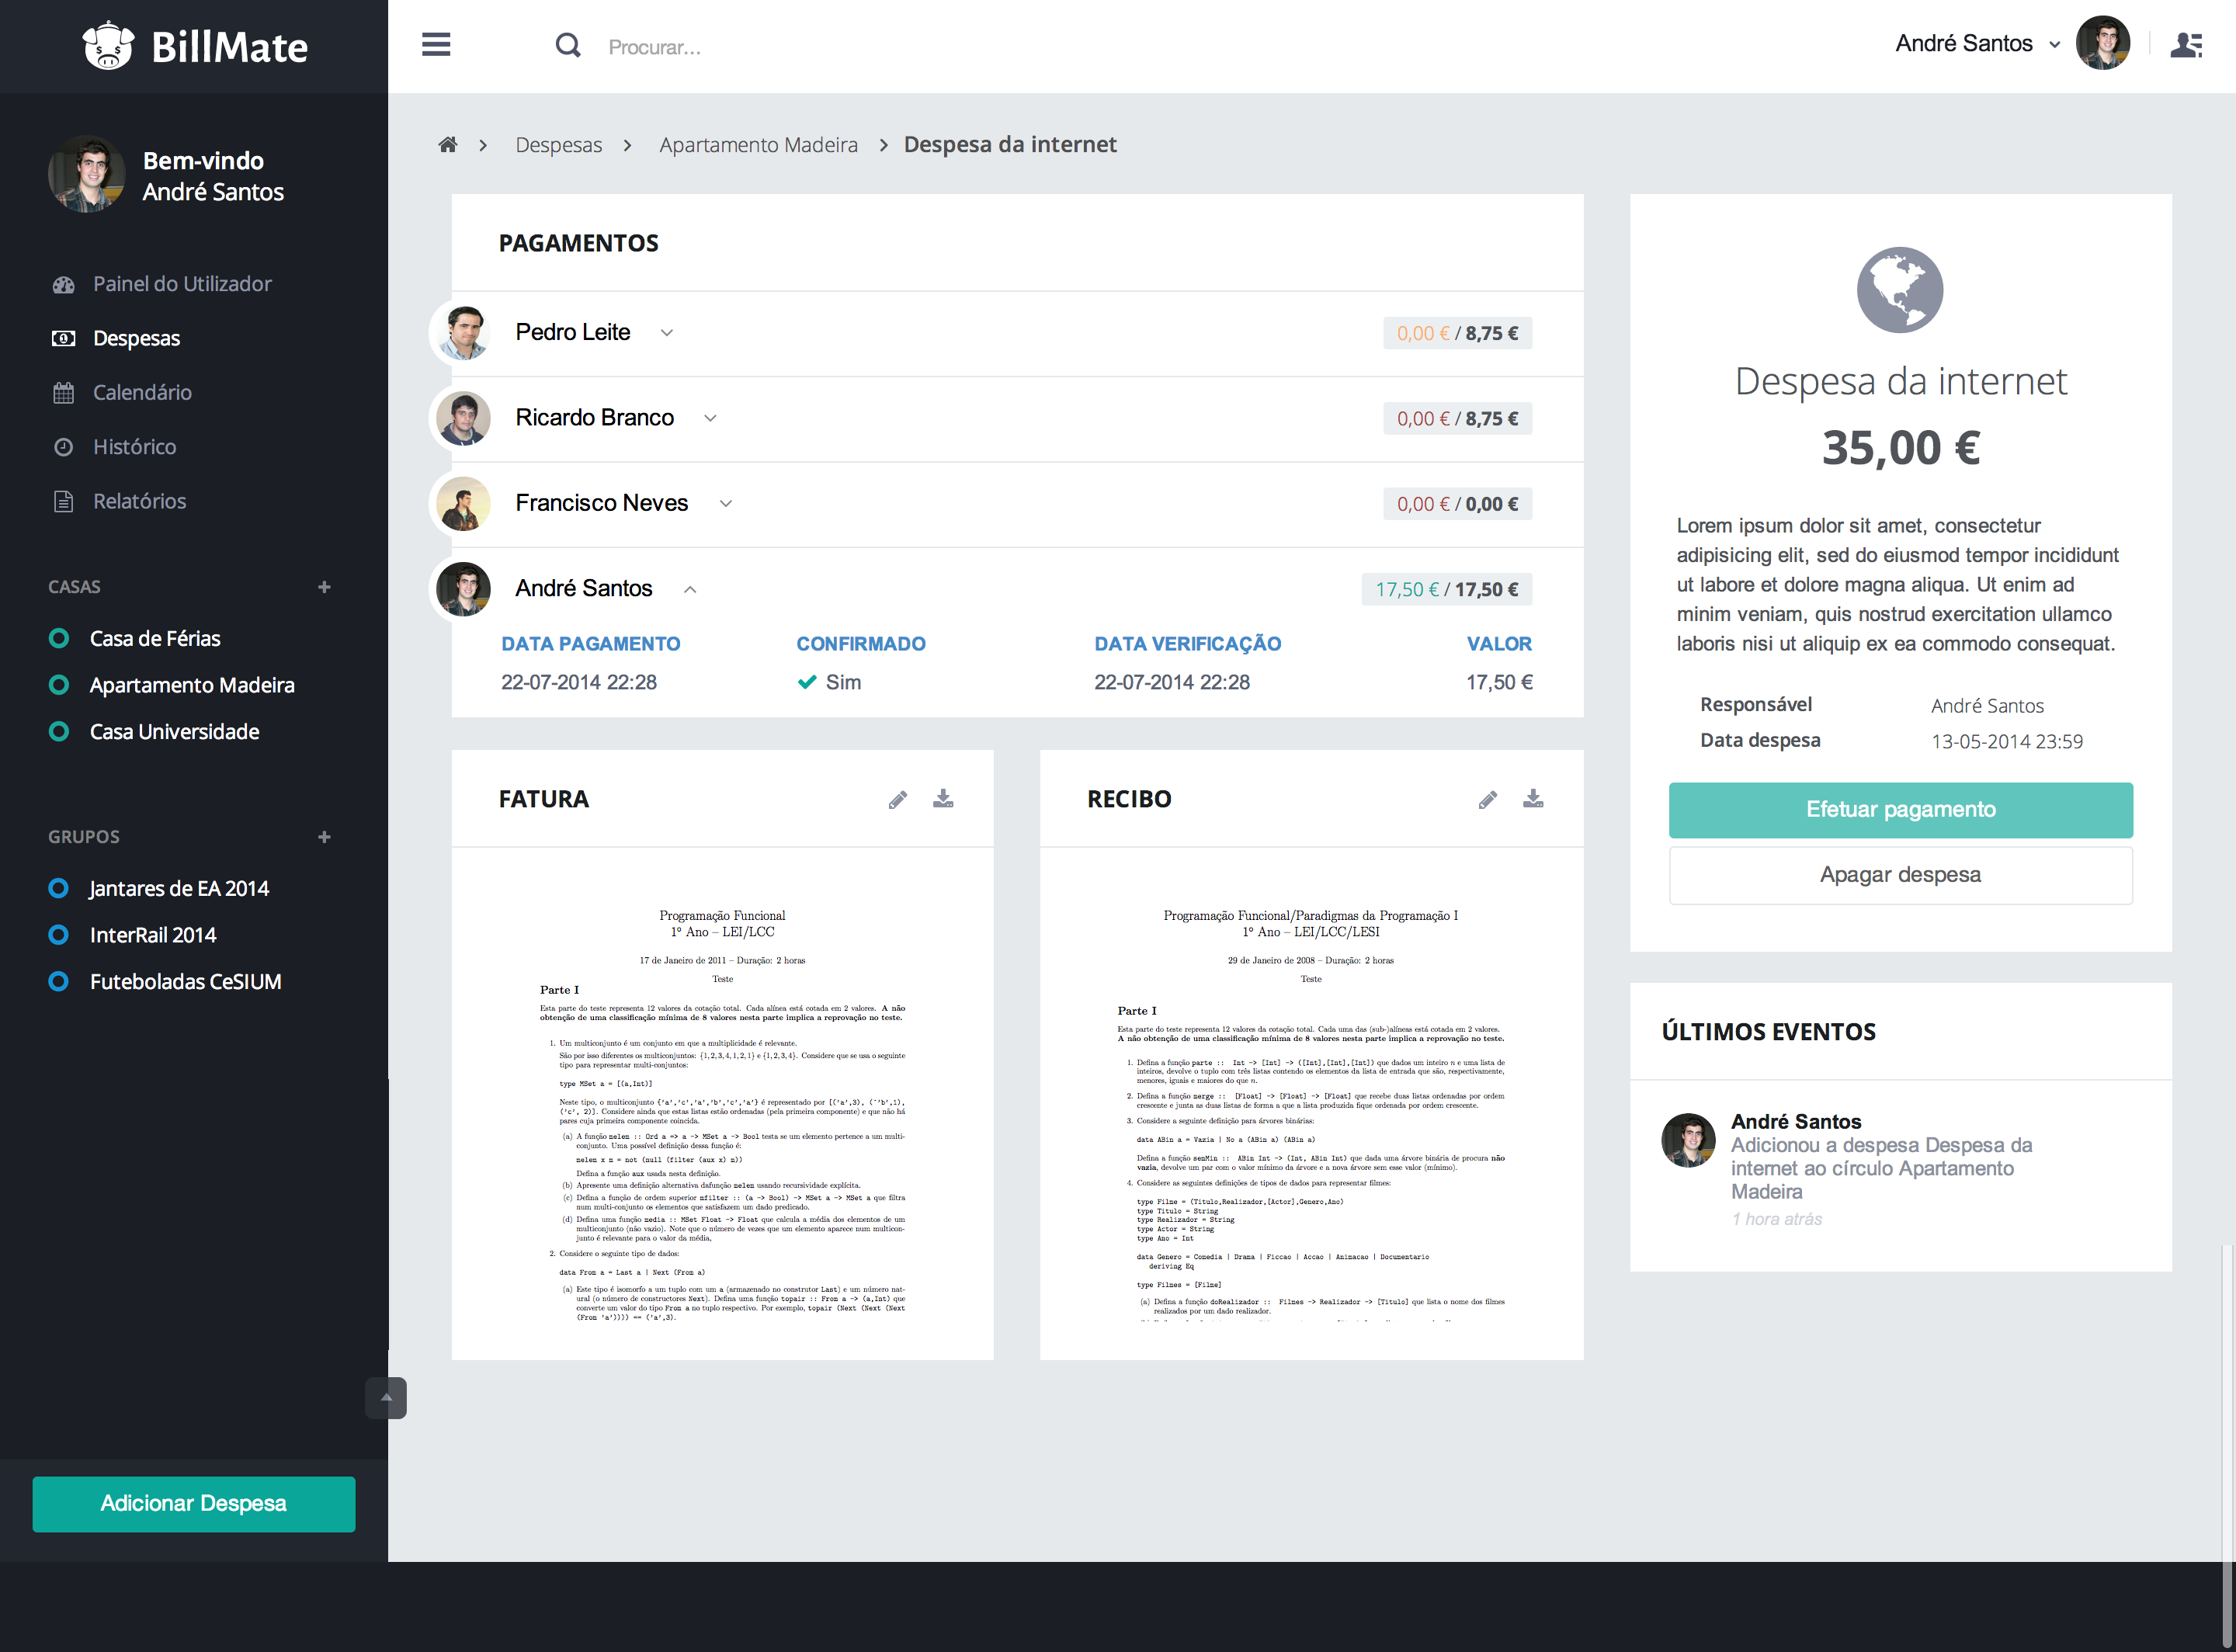
\includegraphics[width=.5\textwidth]{images/andre/expense}
\caption{Página de uma despesa}
}
{
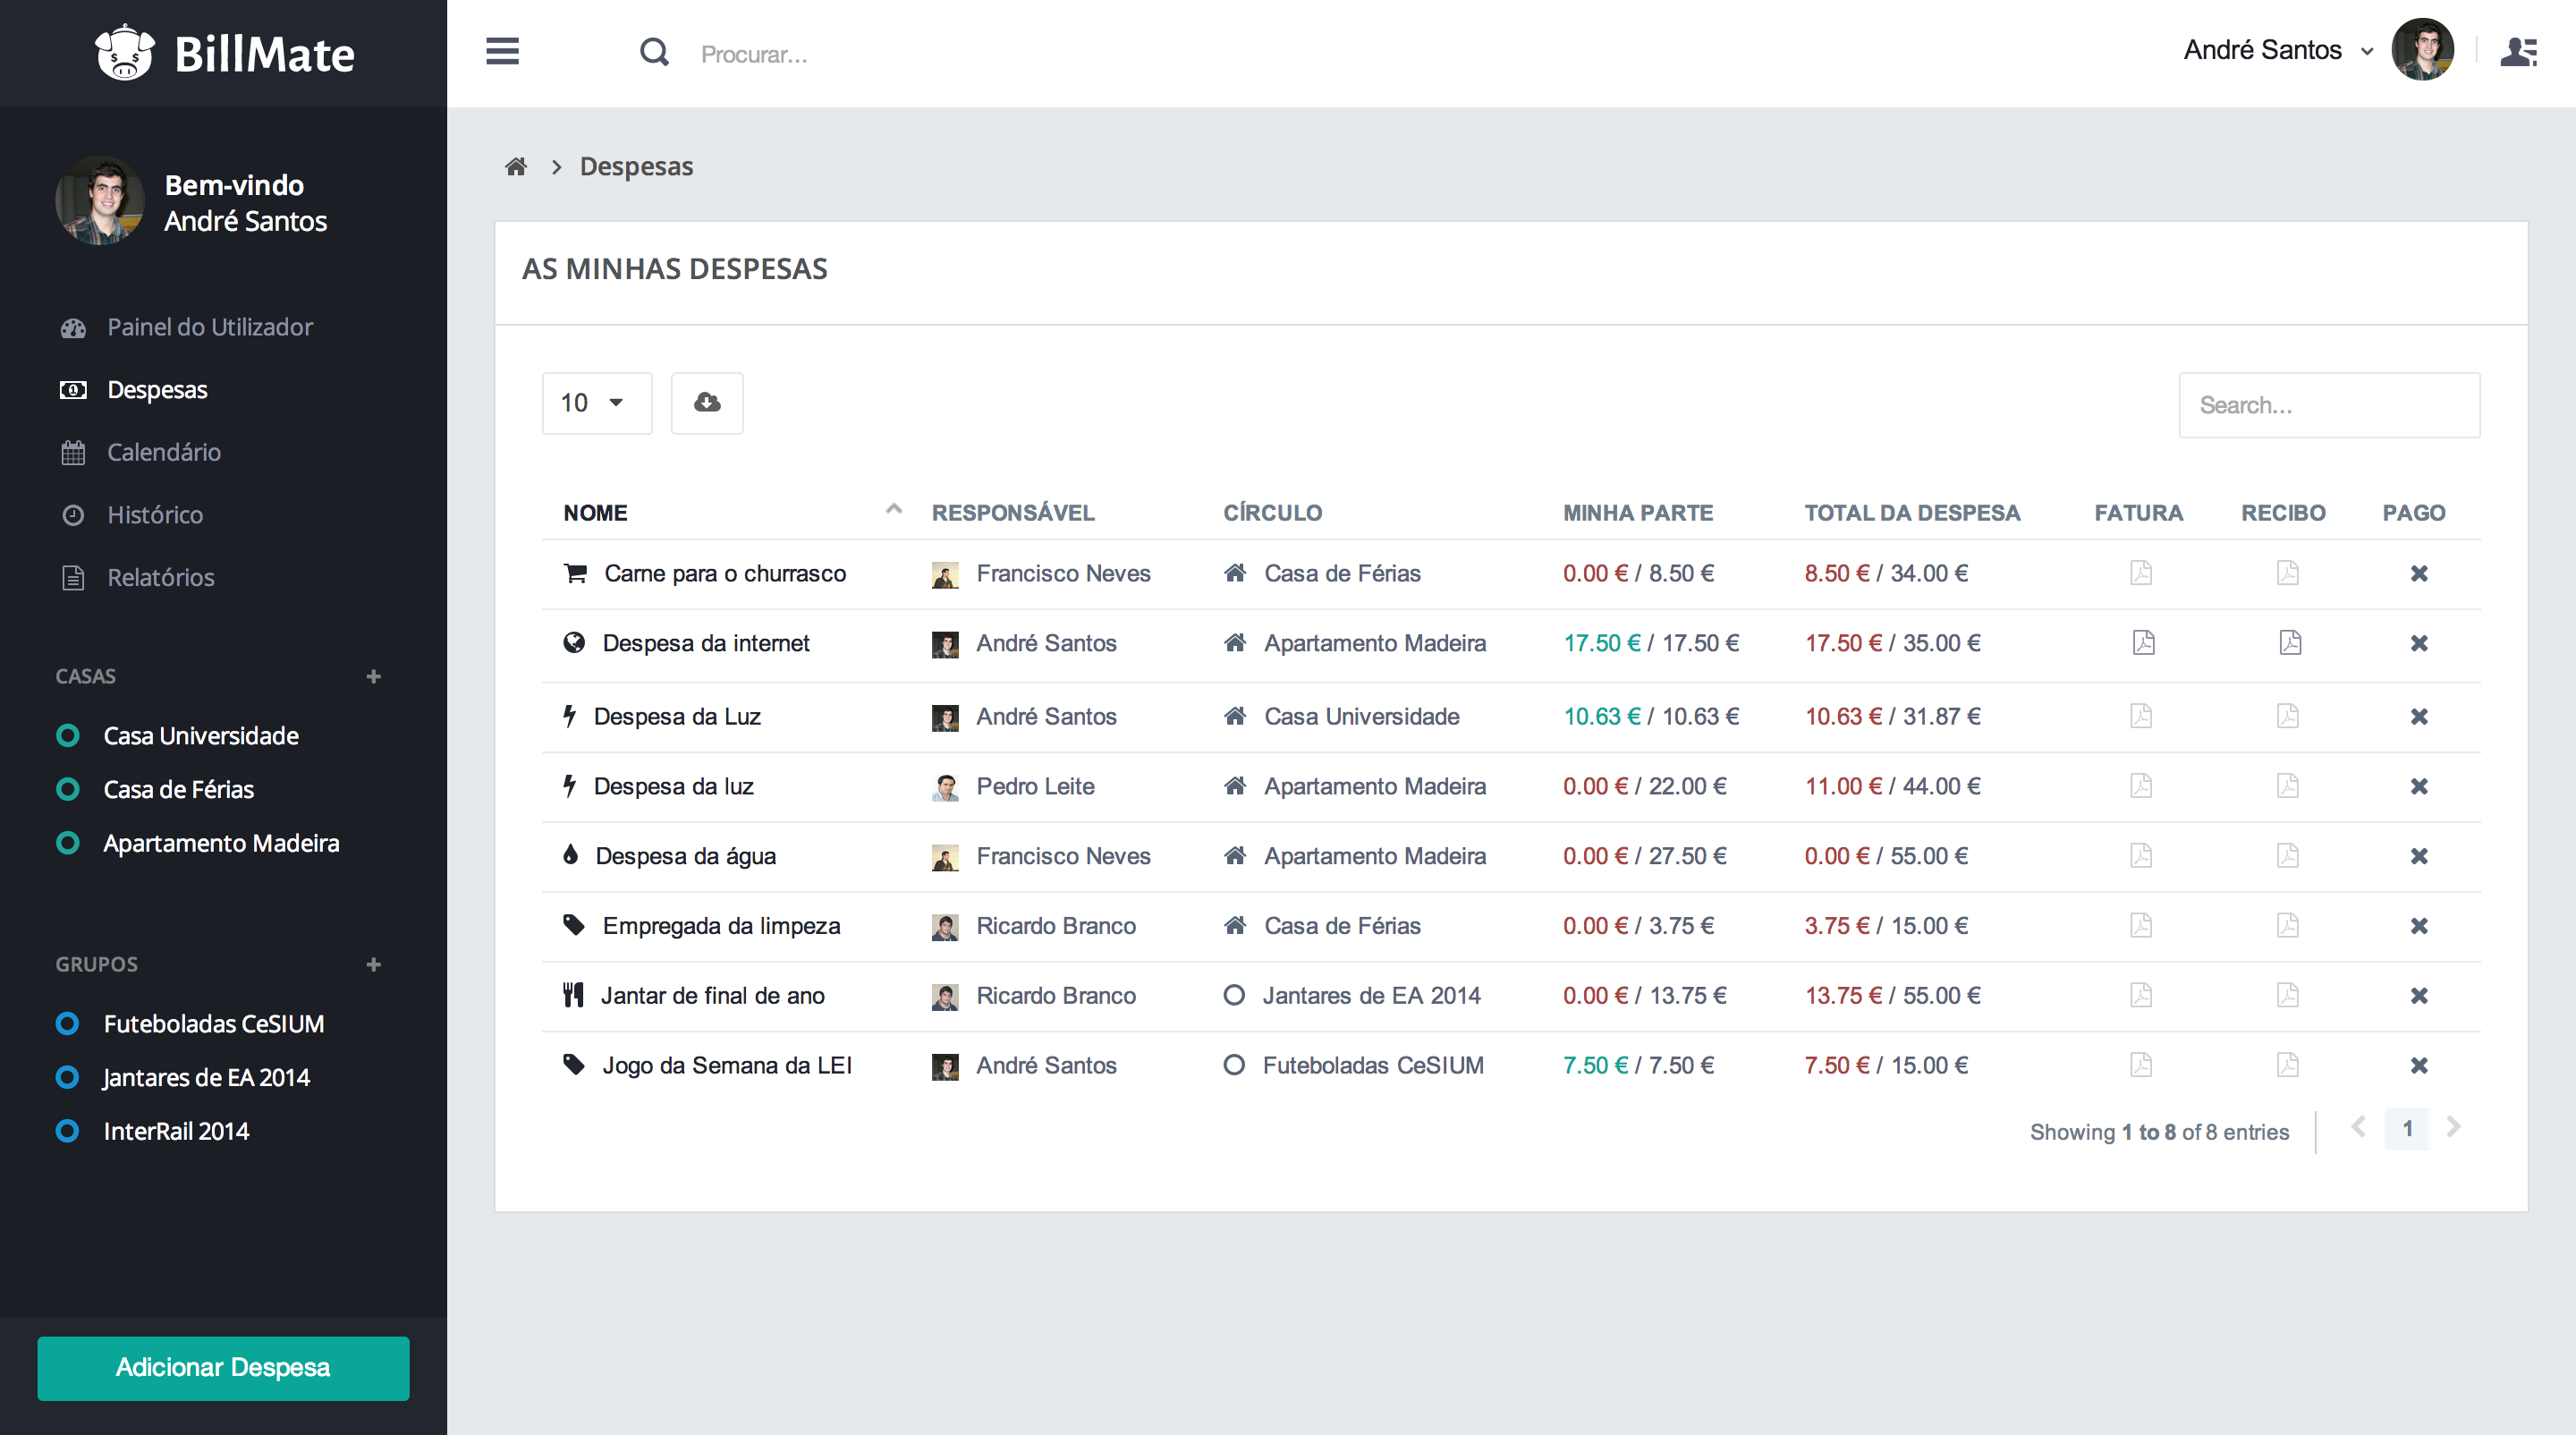
\includegraphics[width=.5\textwidth]{images/andre/expenses}
\caption{Lista de Despesas}
}
\end{figure}

\begin{figure}[ht]
\sidebyside{
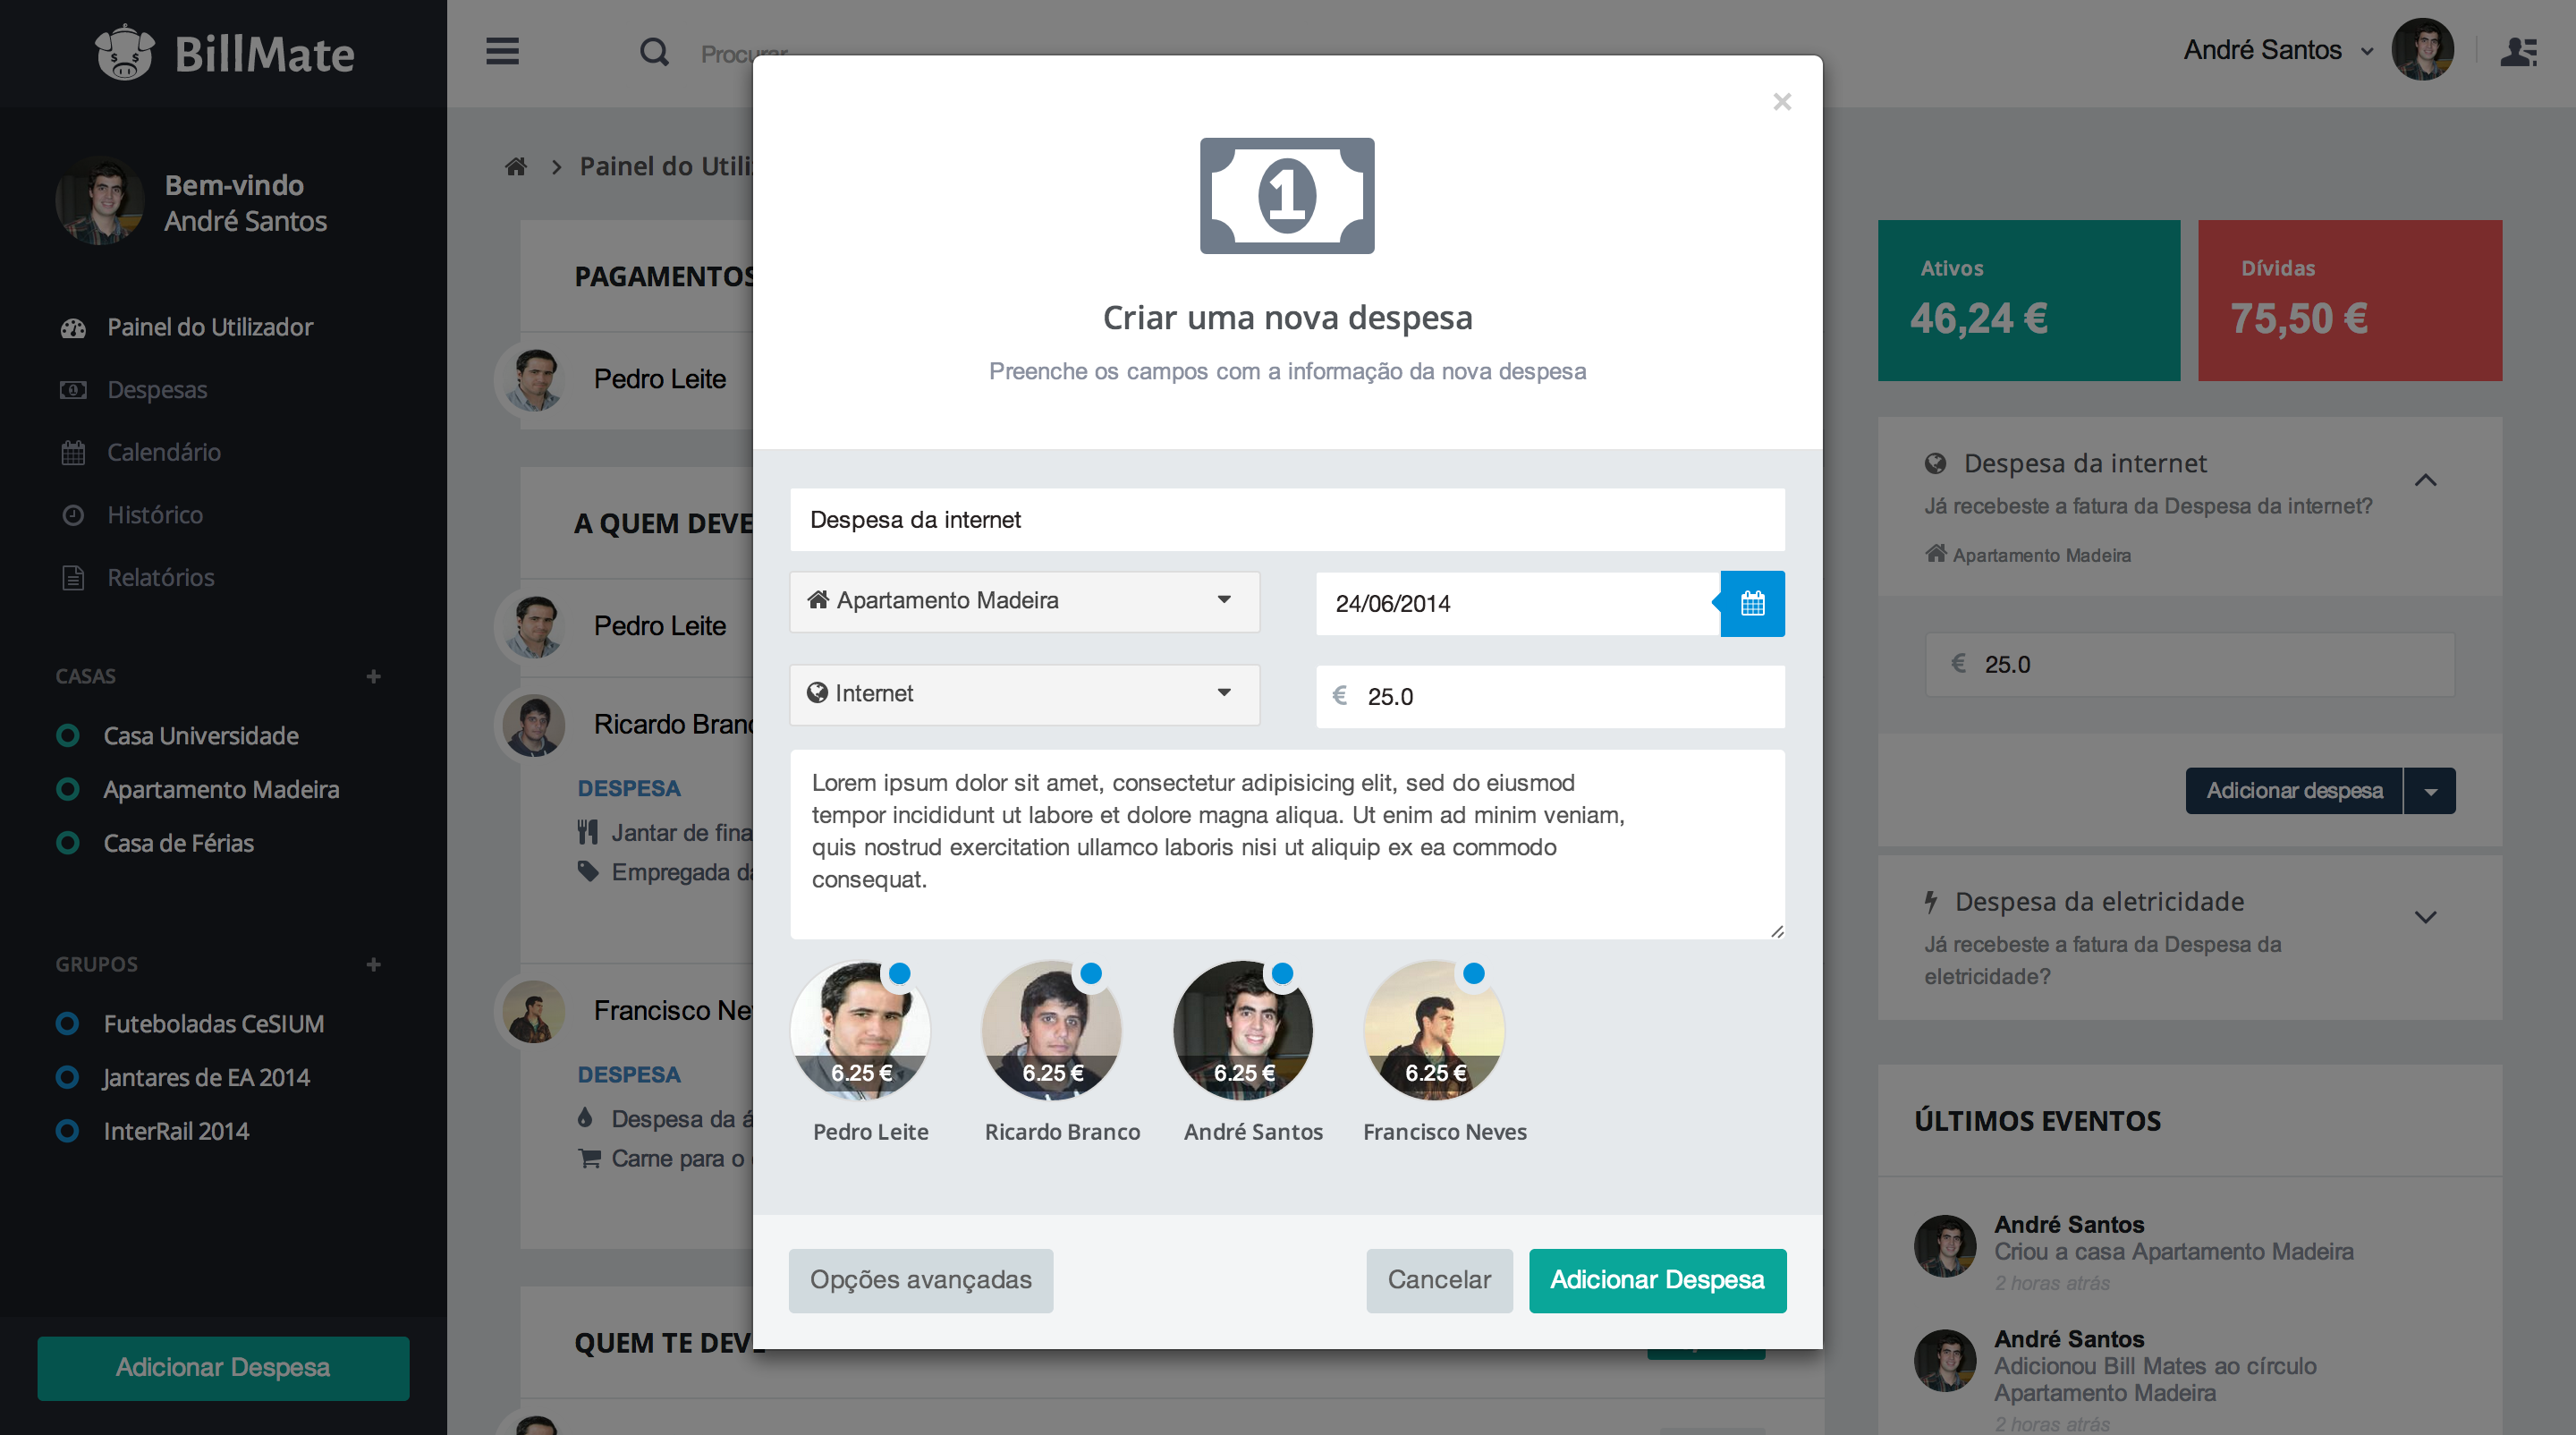
\includegraphics[width=.5\textwidth]{images/andre/create_regular_expense}
\caption{Criar despesa regular}
}
{
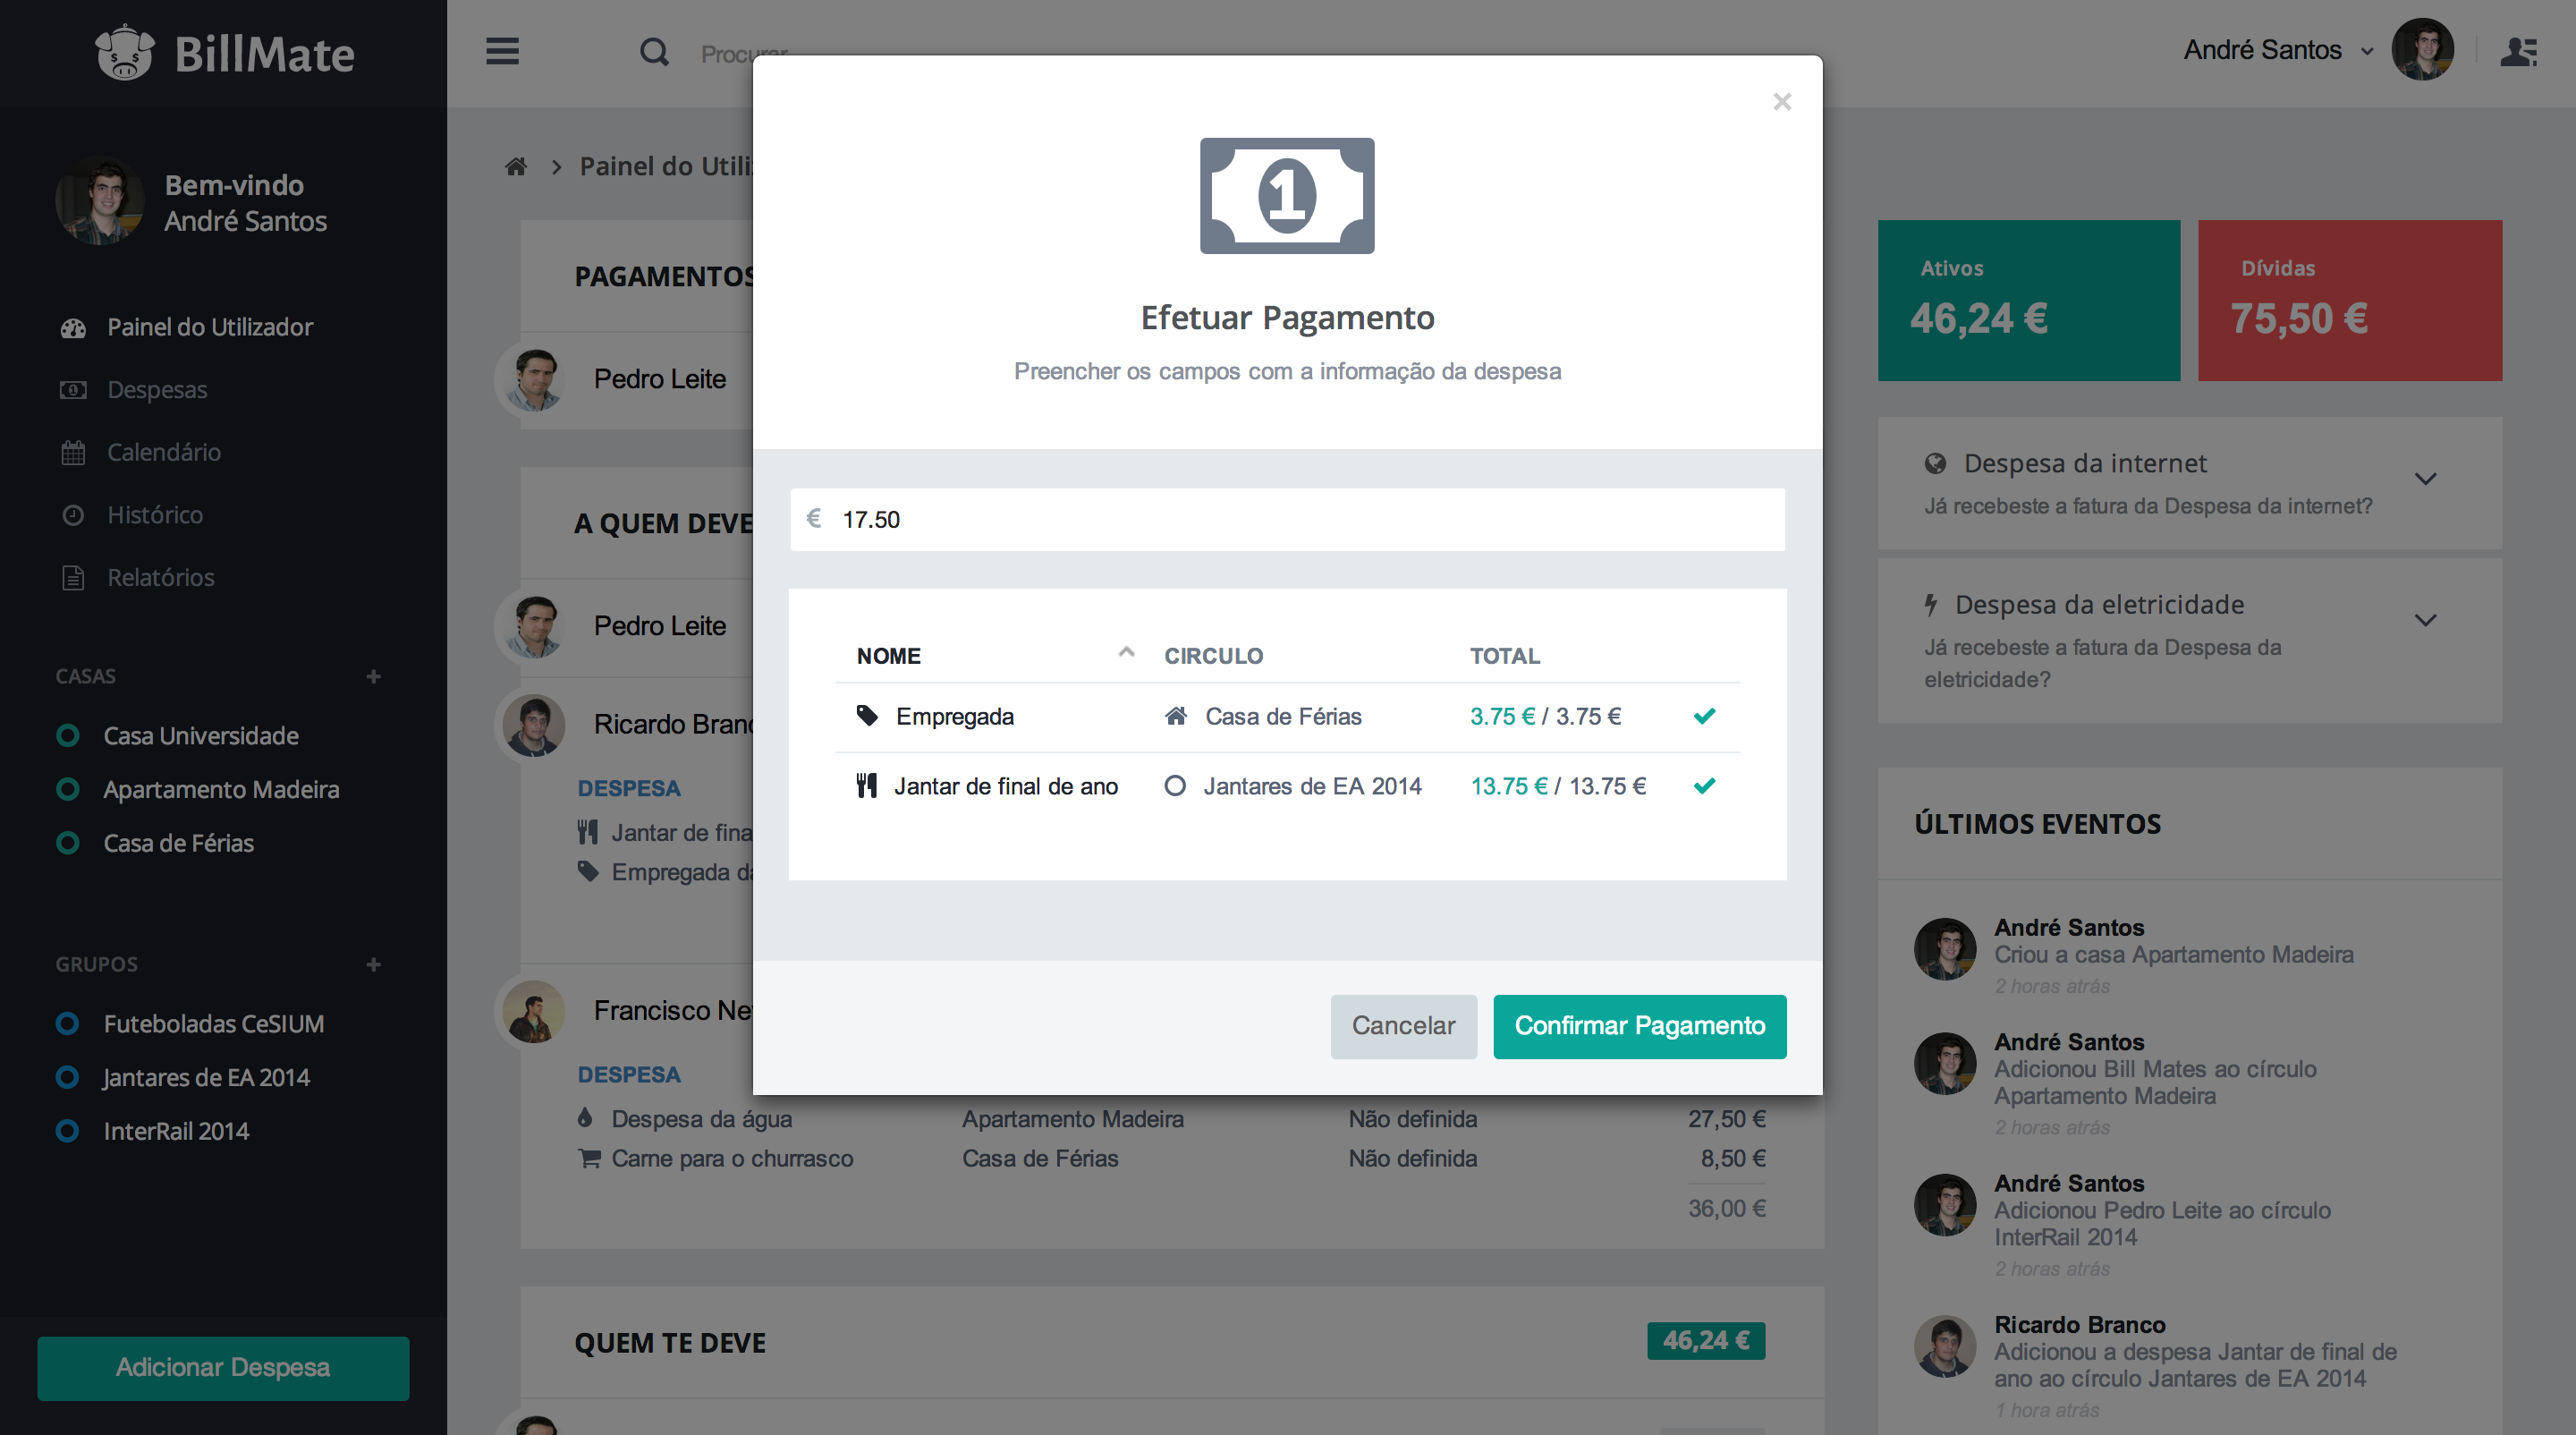
\includegraphics[width=.5\textwidth]{images/andre/payment}
\caption{Confirmar pagamento}
}
\end{figure}

\begin{figure}[ht]
\sidebyside{
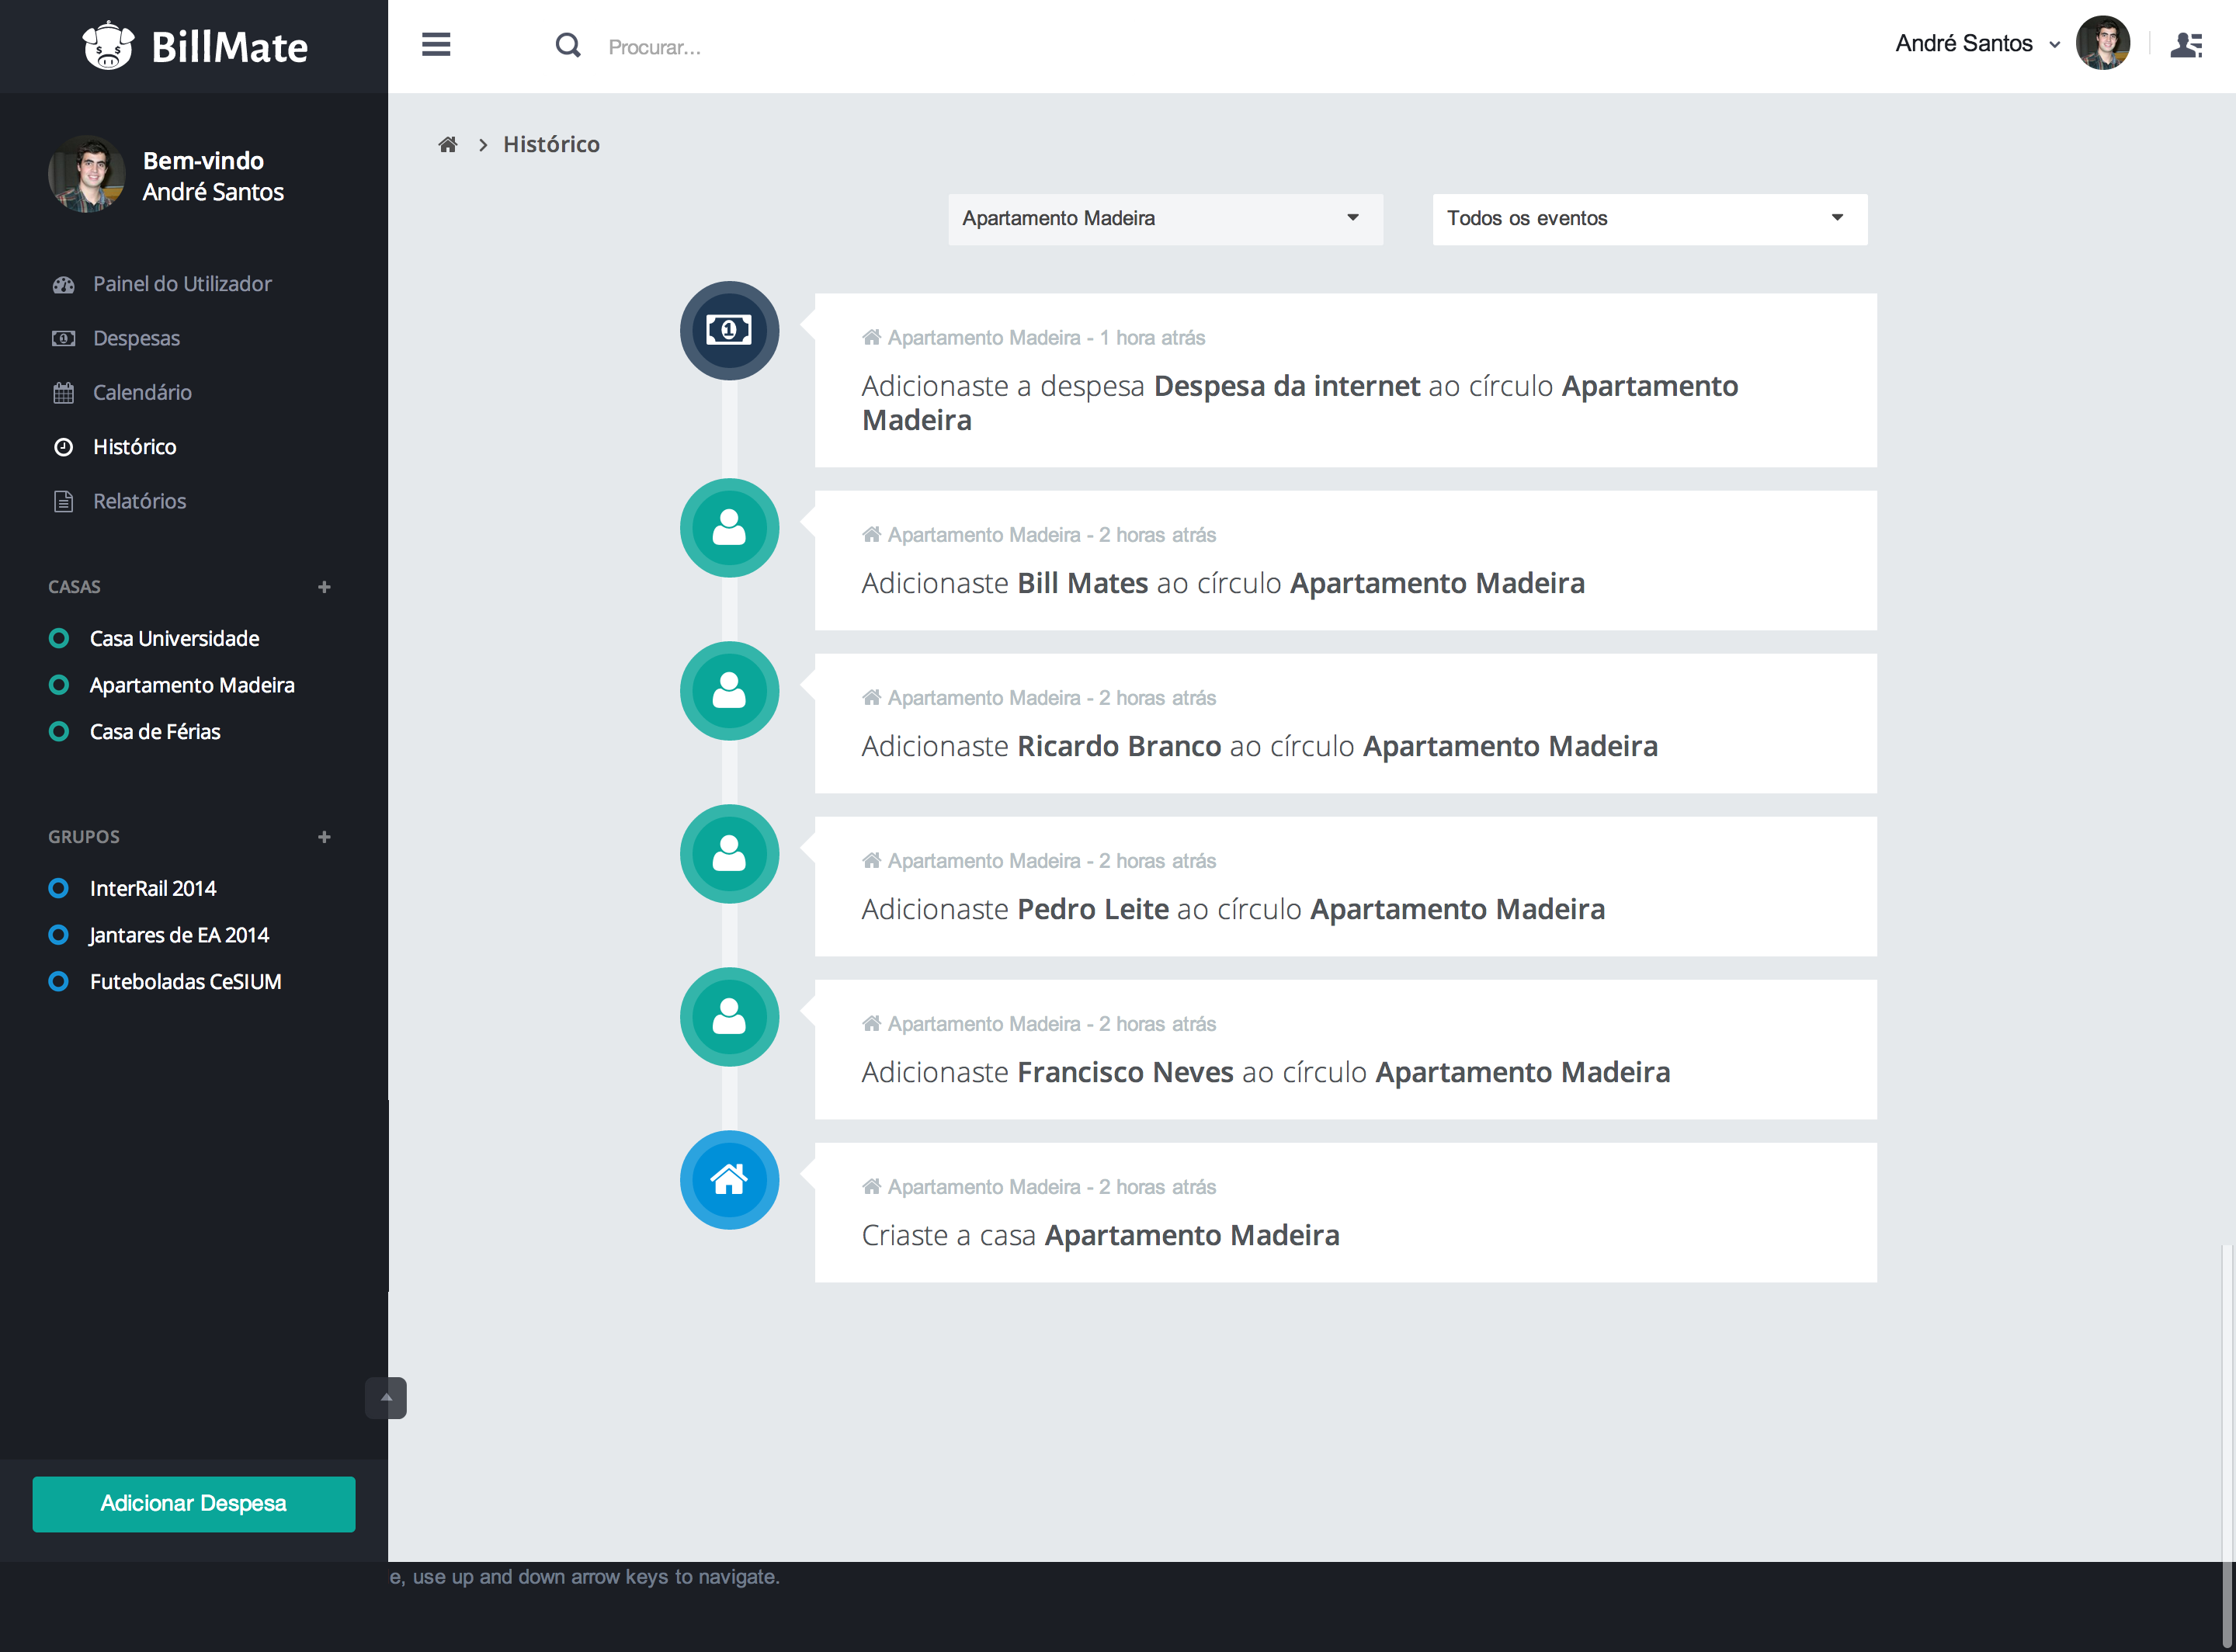
\includegraphics[width=.5\textwidth]{images/andre/history}
\caption{Histórico}
}
{
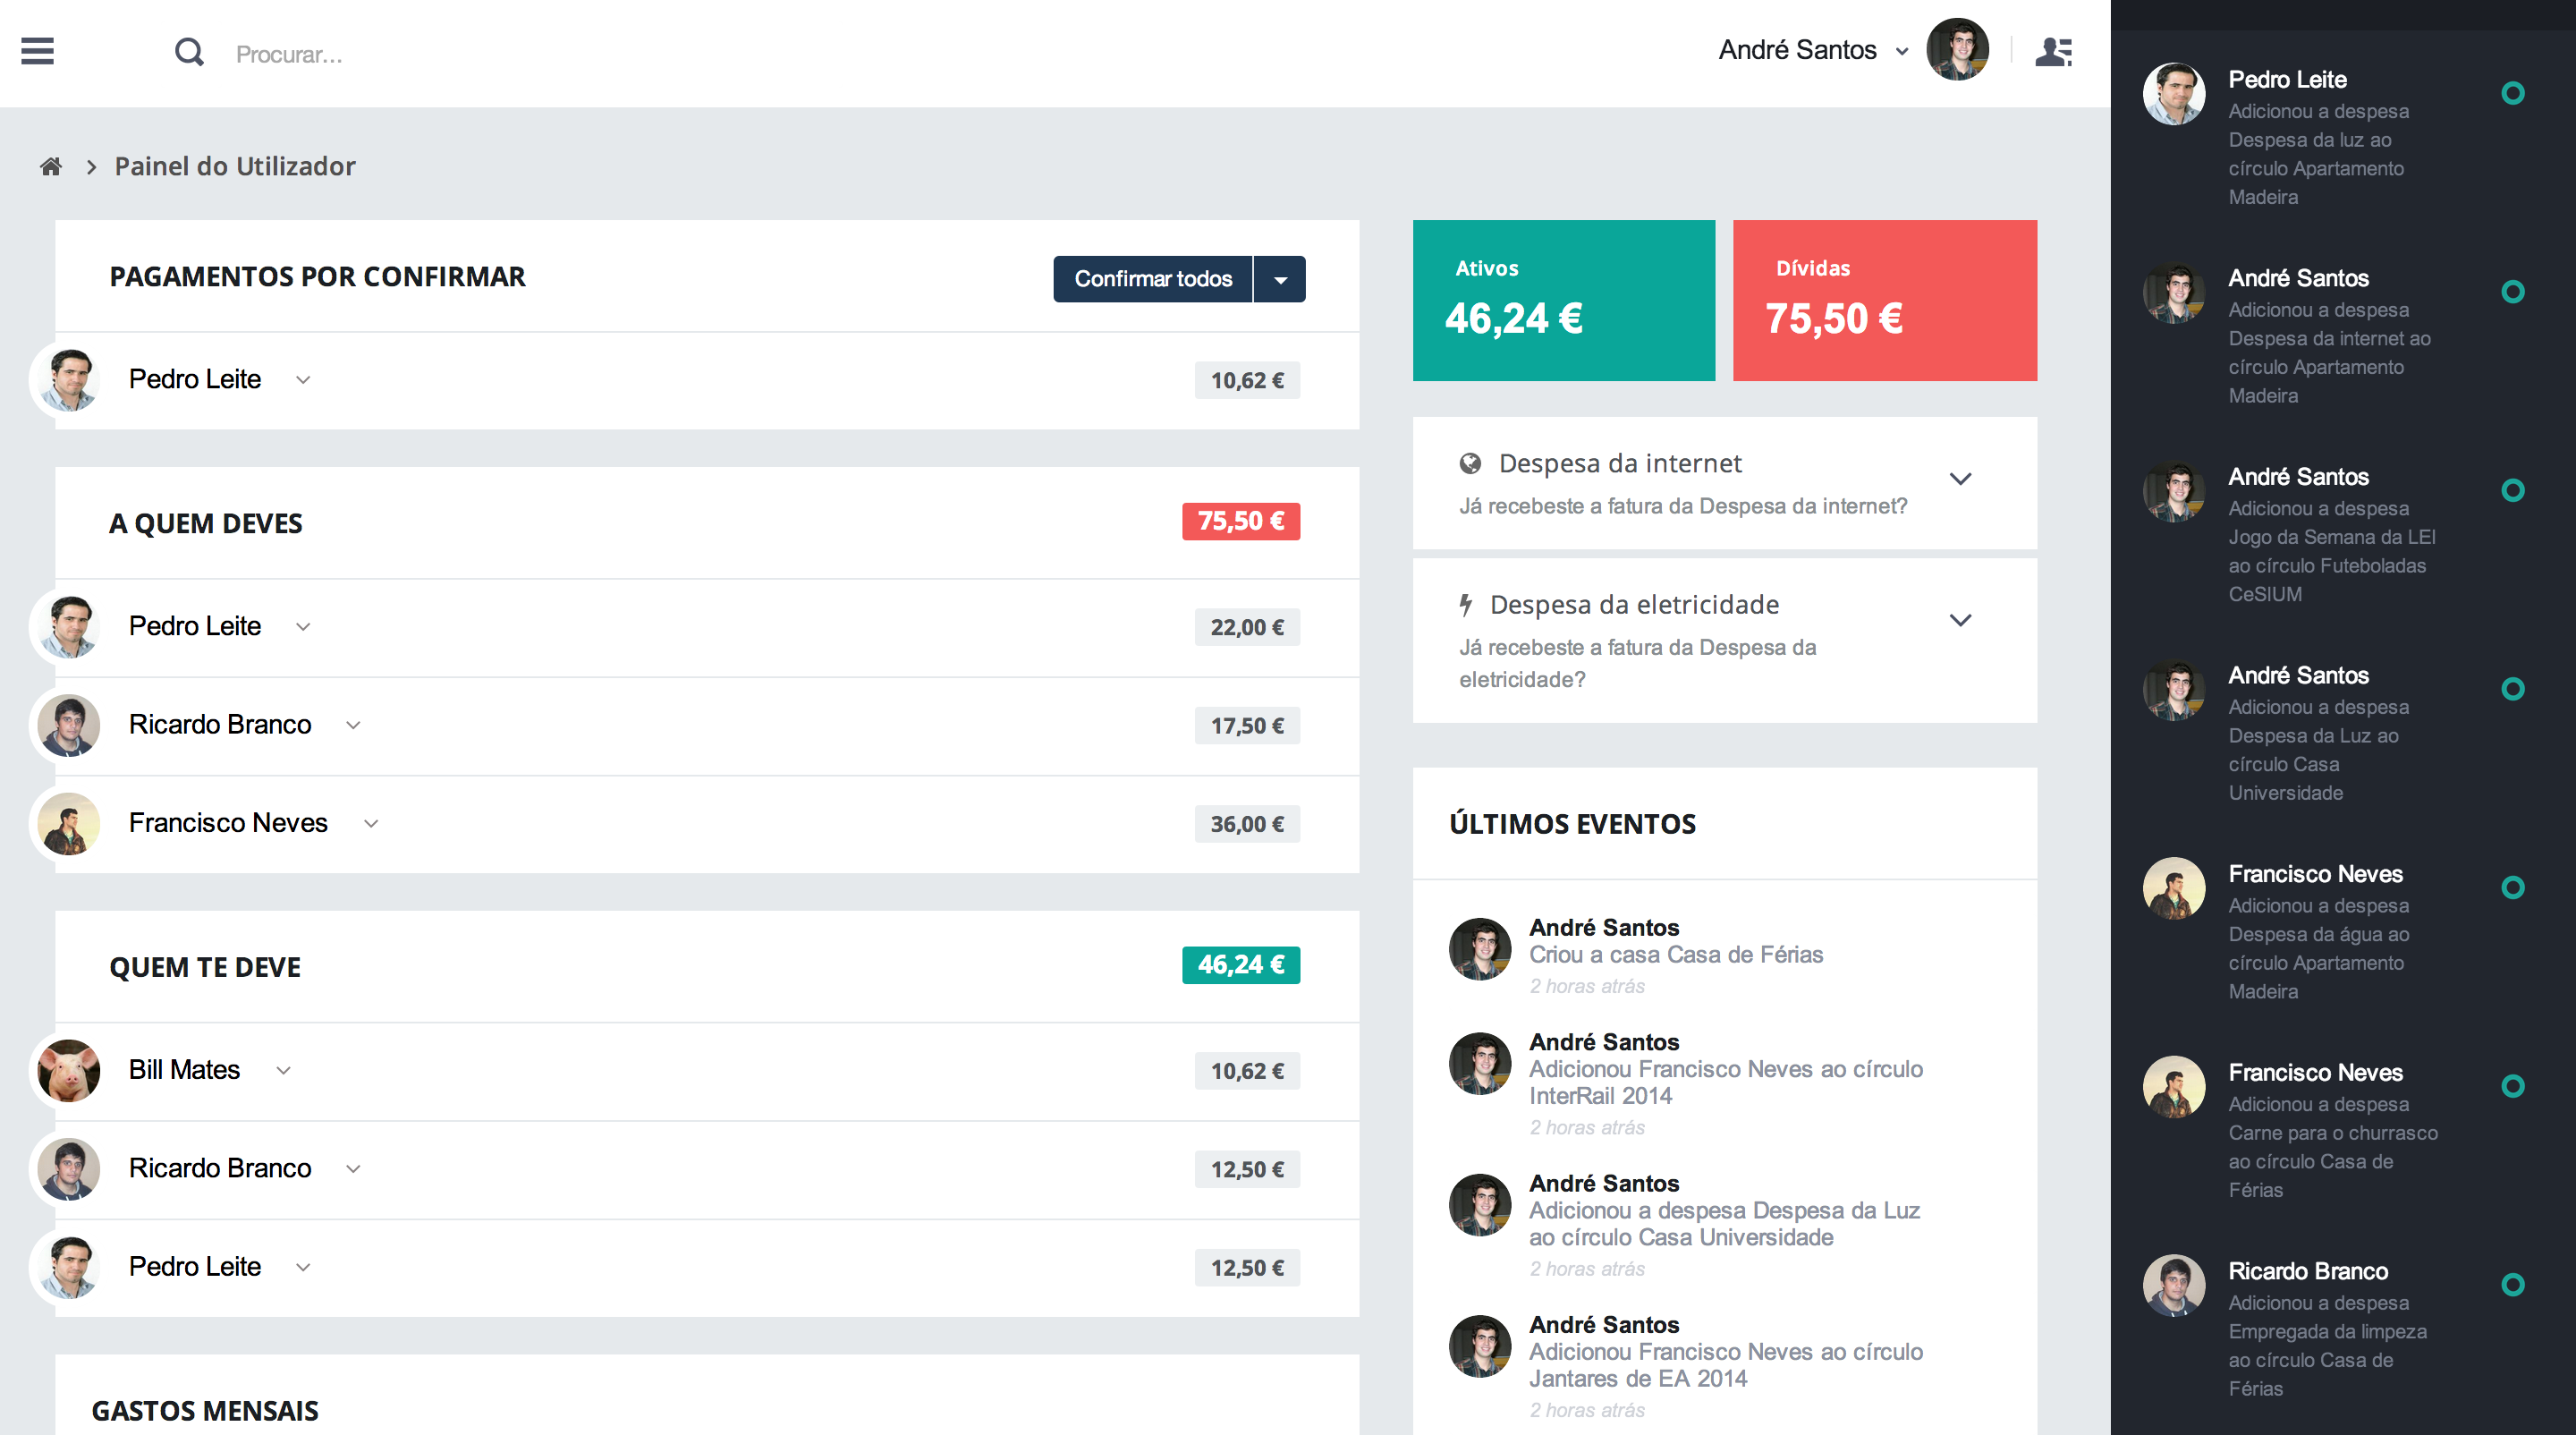
\includegraphics[width=.5\textwidth]{images/andre/notifications}
\caption{Notificações}
}
\end{figure}

\begin{figure}[ht]
\sidebyside{
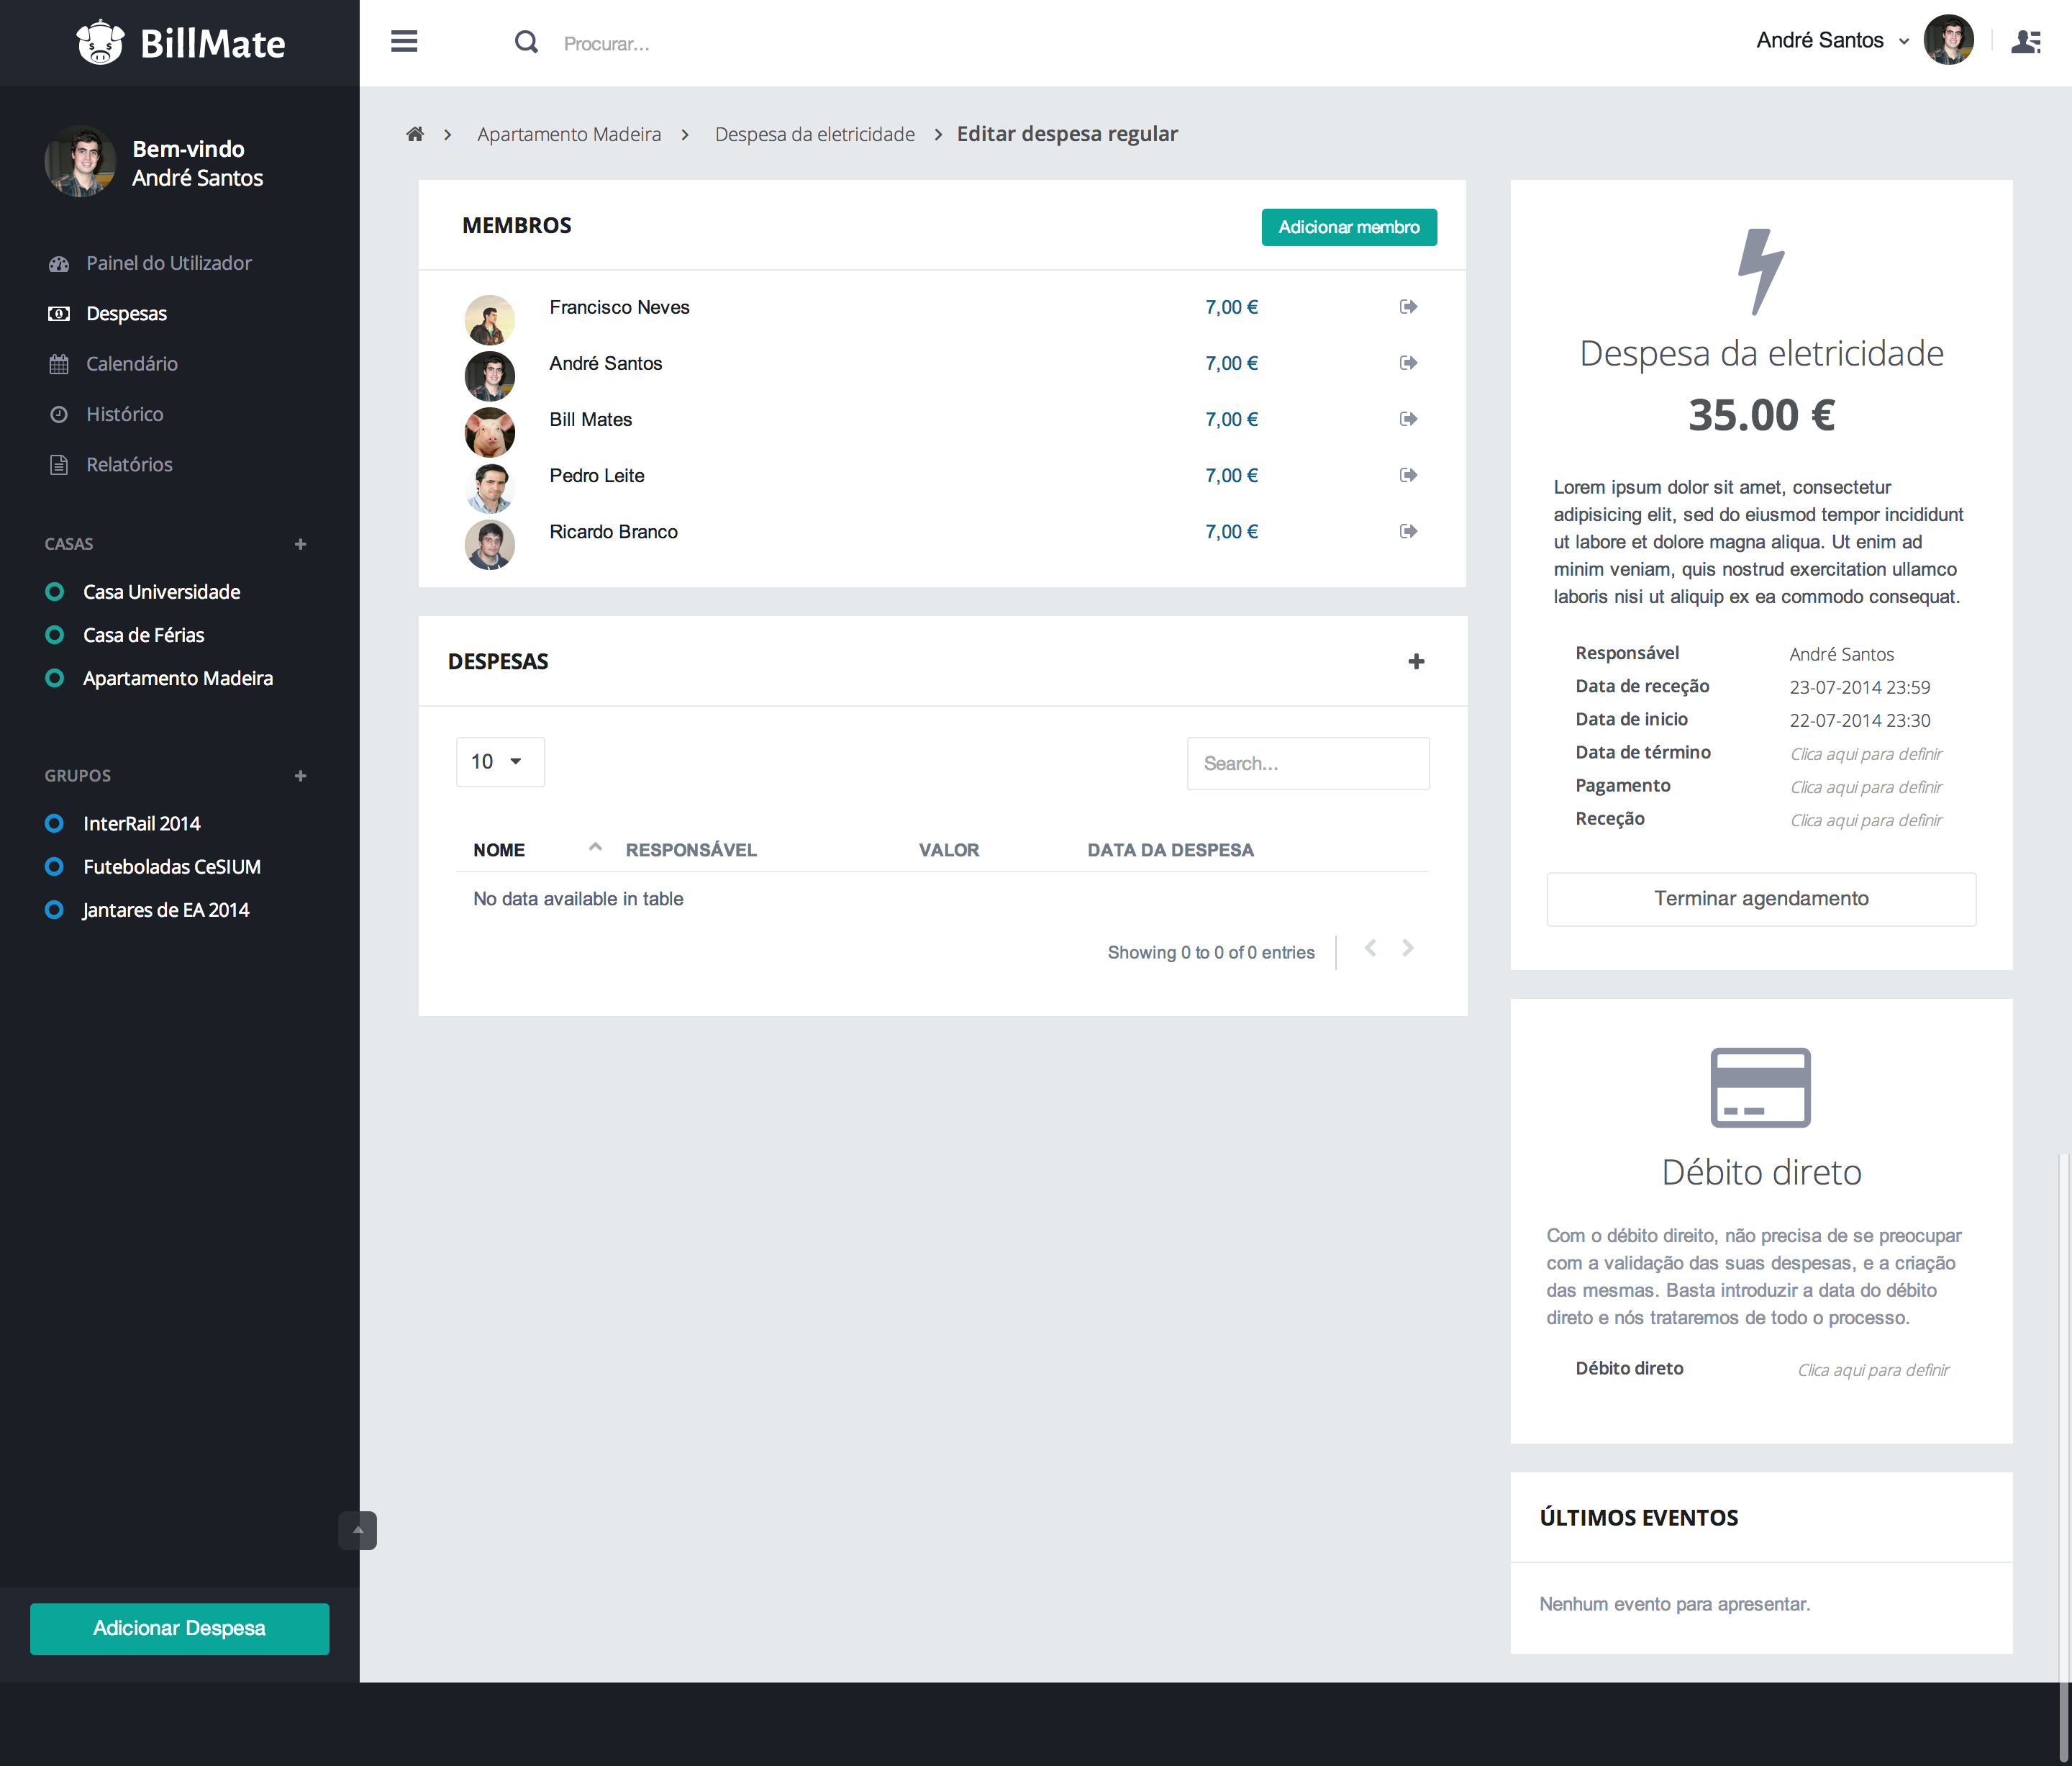
\includegraphics[width=.5\textwidth]{images/andre/regular_expense}
\caption{Editar despesa regular}
}
{
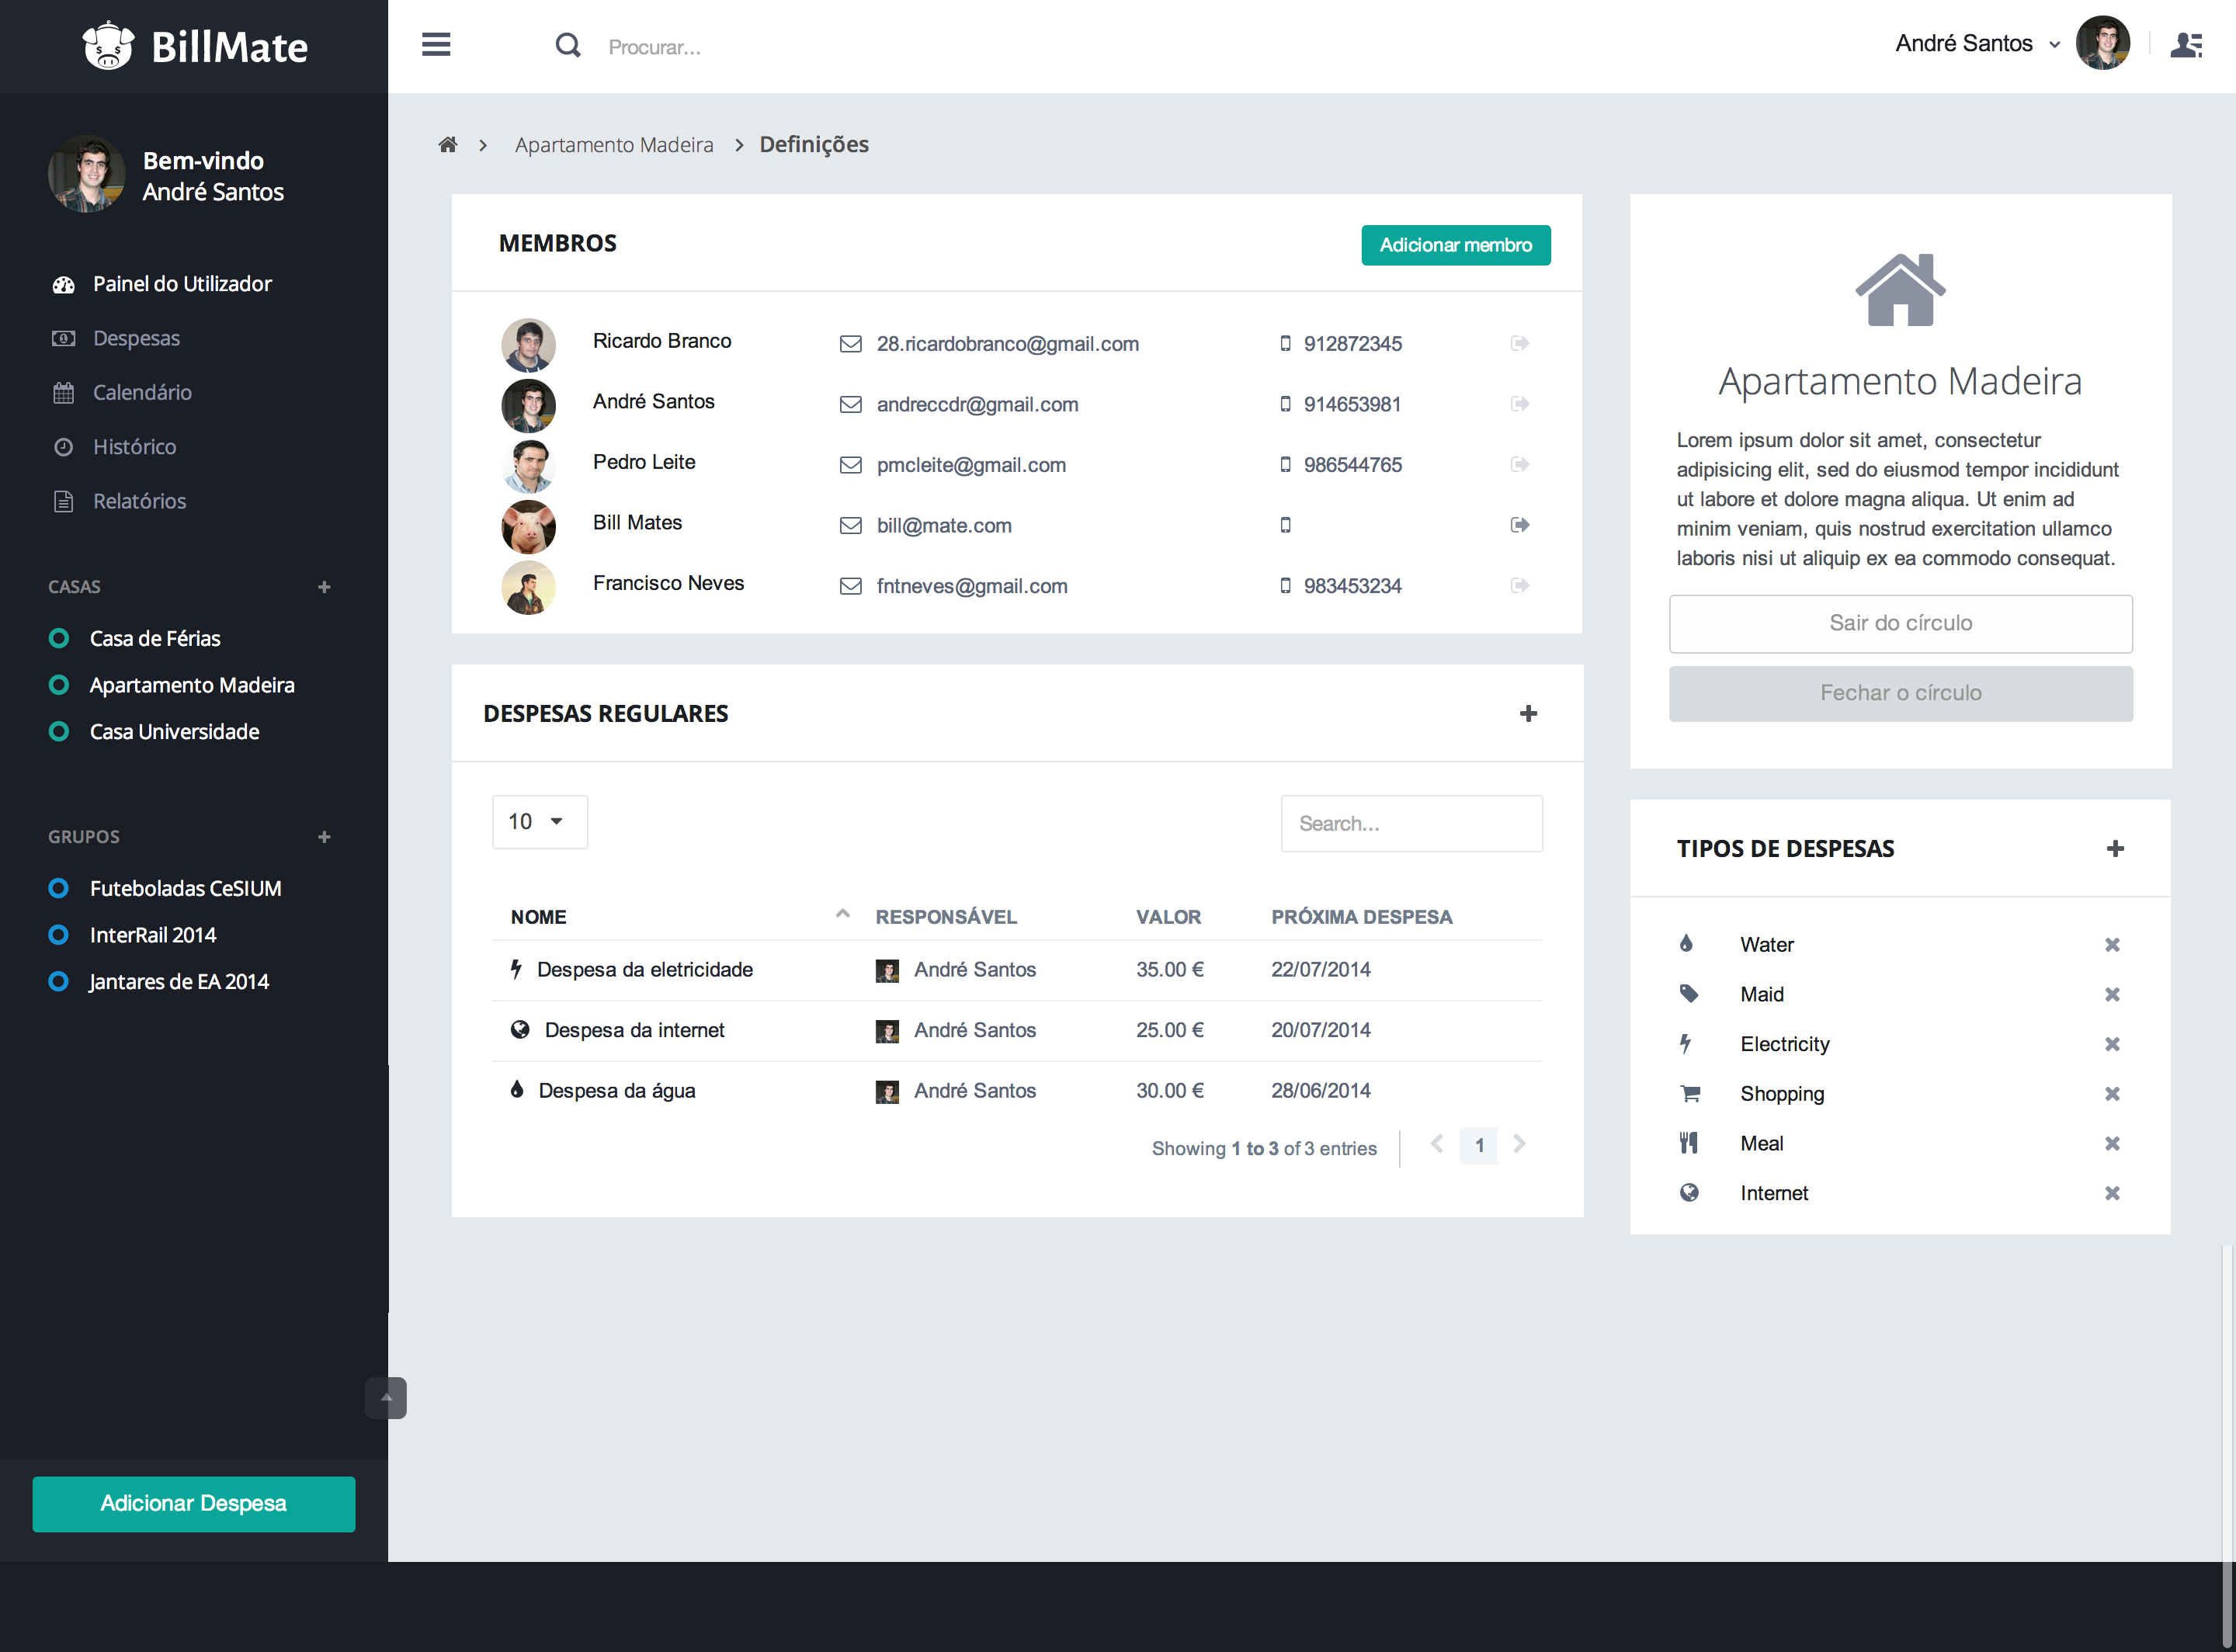
\includegraphics[width=.5\textwidth]{images/andre/settings_circle}
\caption{Definições de um círculo}
}
\end{figure}

\begin{figure}[ht]
\sidebyside{
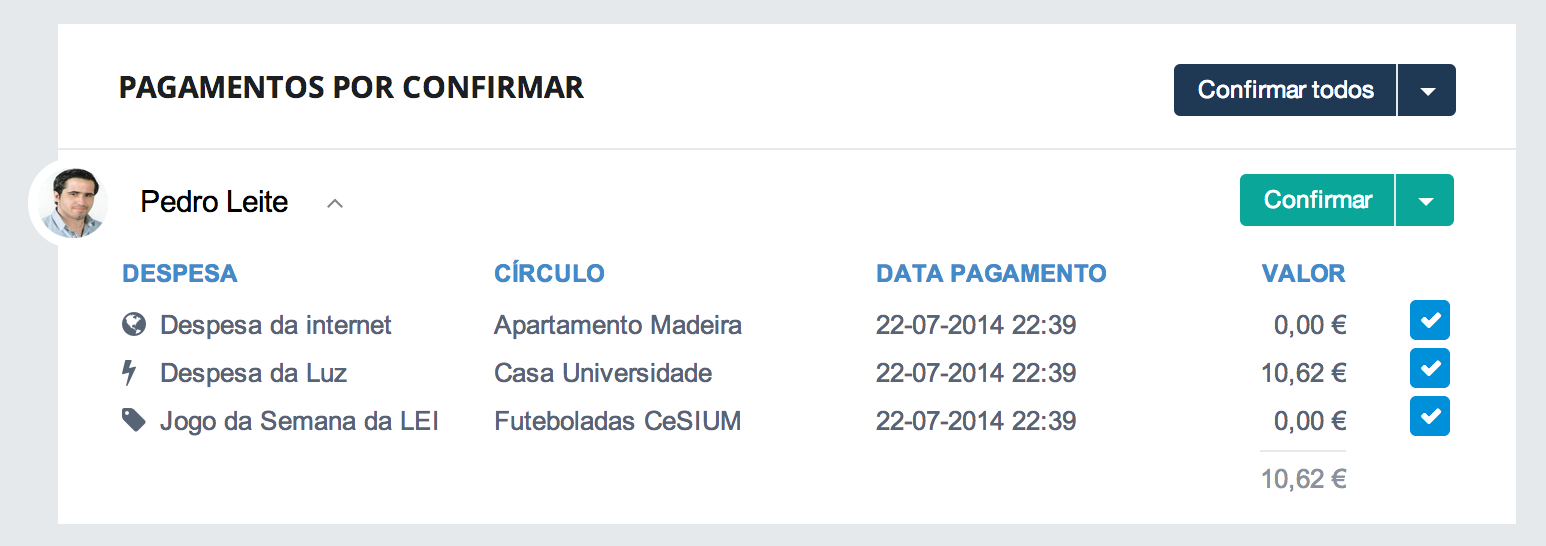
\includegraphics[width=.5\textwidth]{images/andre/confirmarpagamentos}
\caption{Confirmar Pagamentos}
}
{
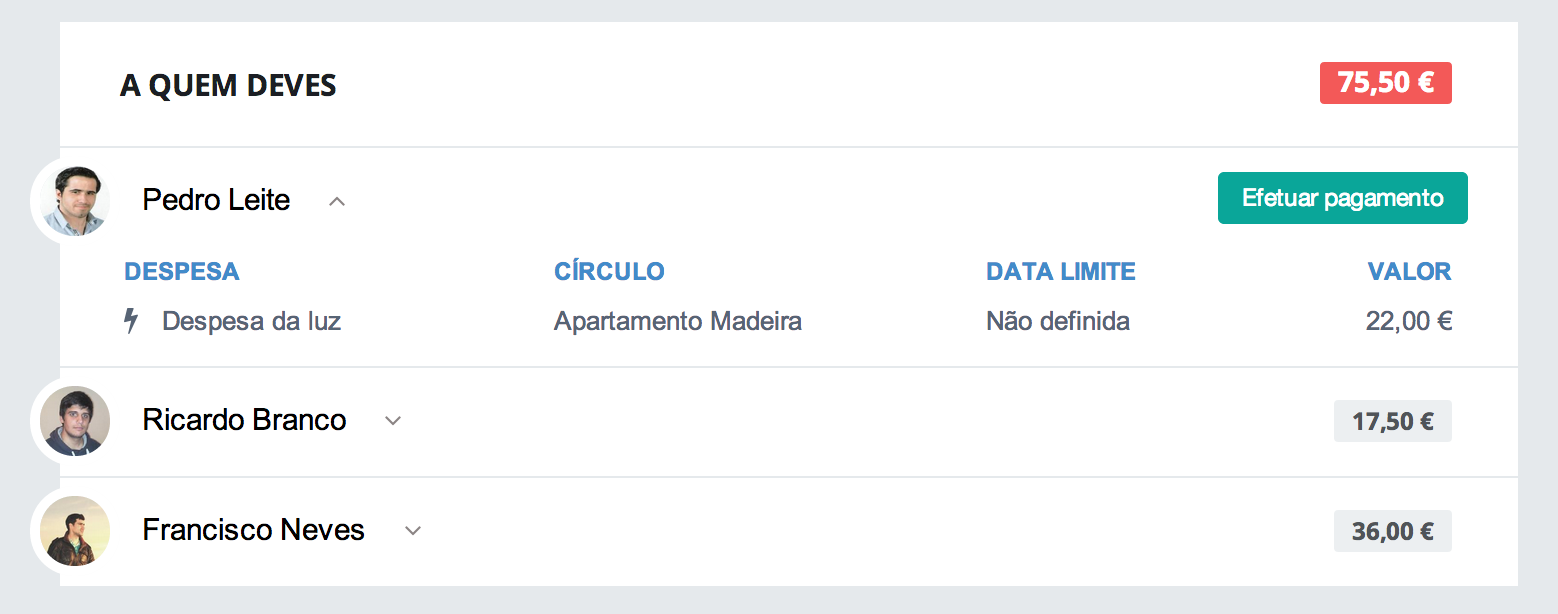
\includegraphics[width=.5\textwidth]{images/andre/dividas}
\caption{Listar dívidas}
}
\end{figure}

\begin{figure}[ht]
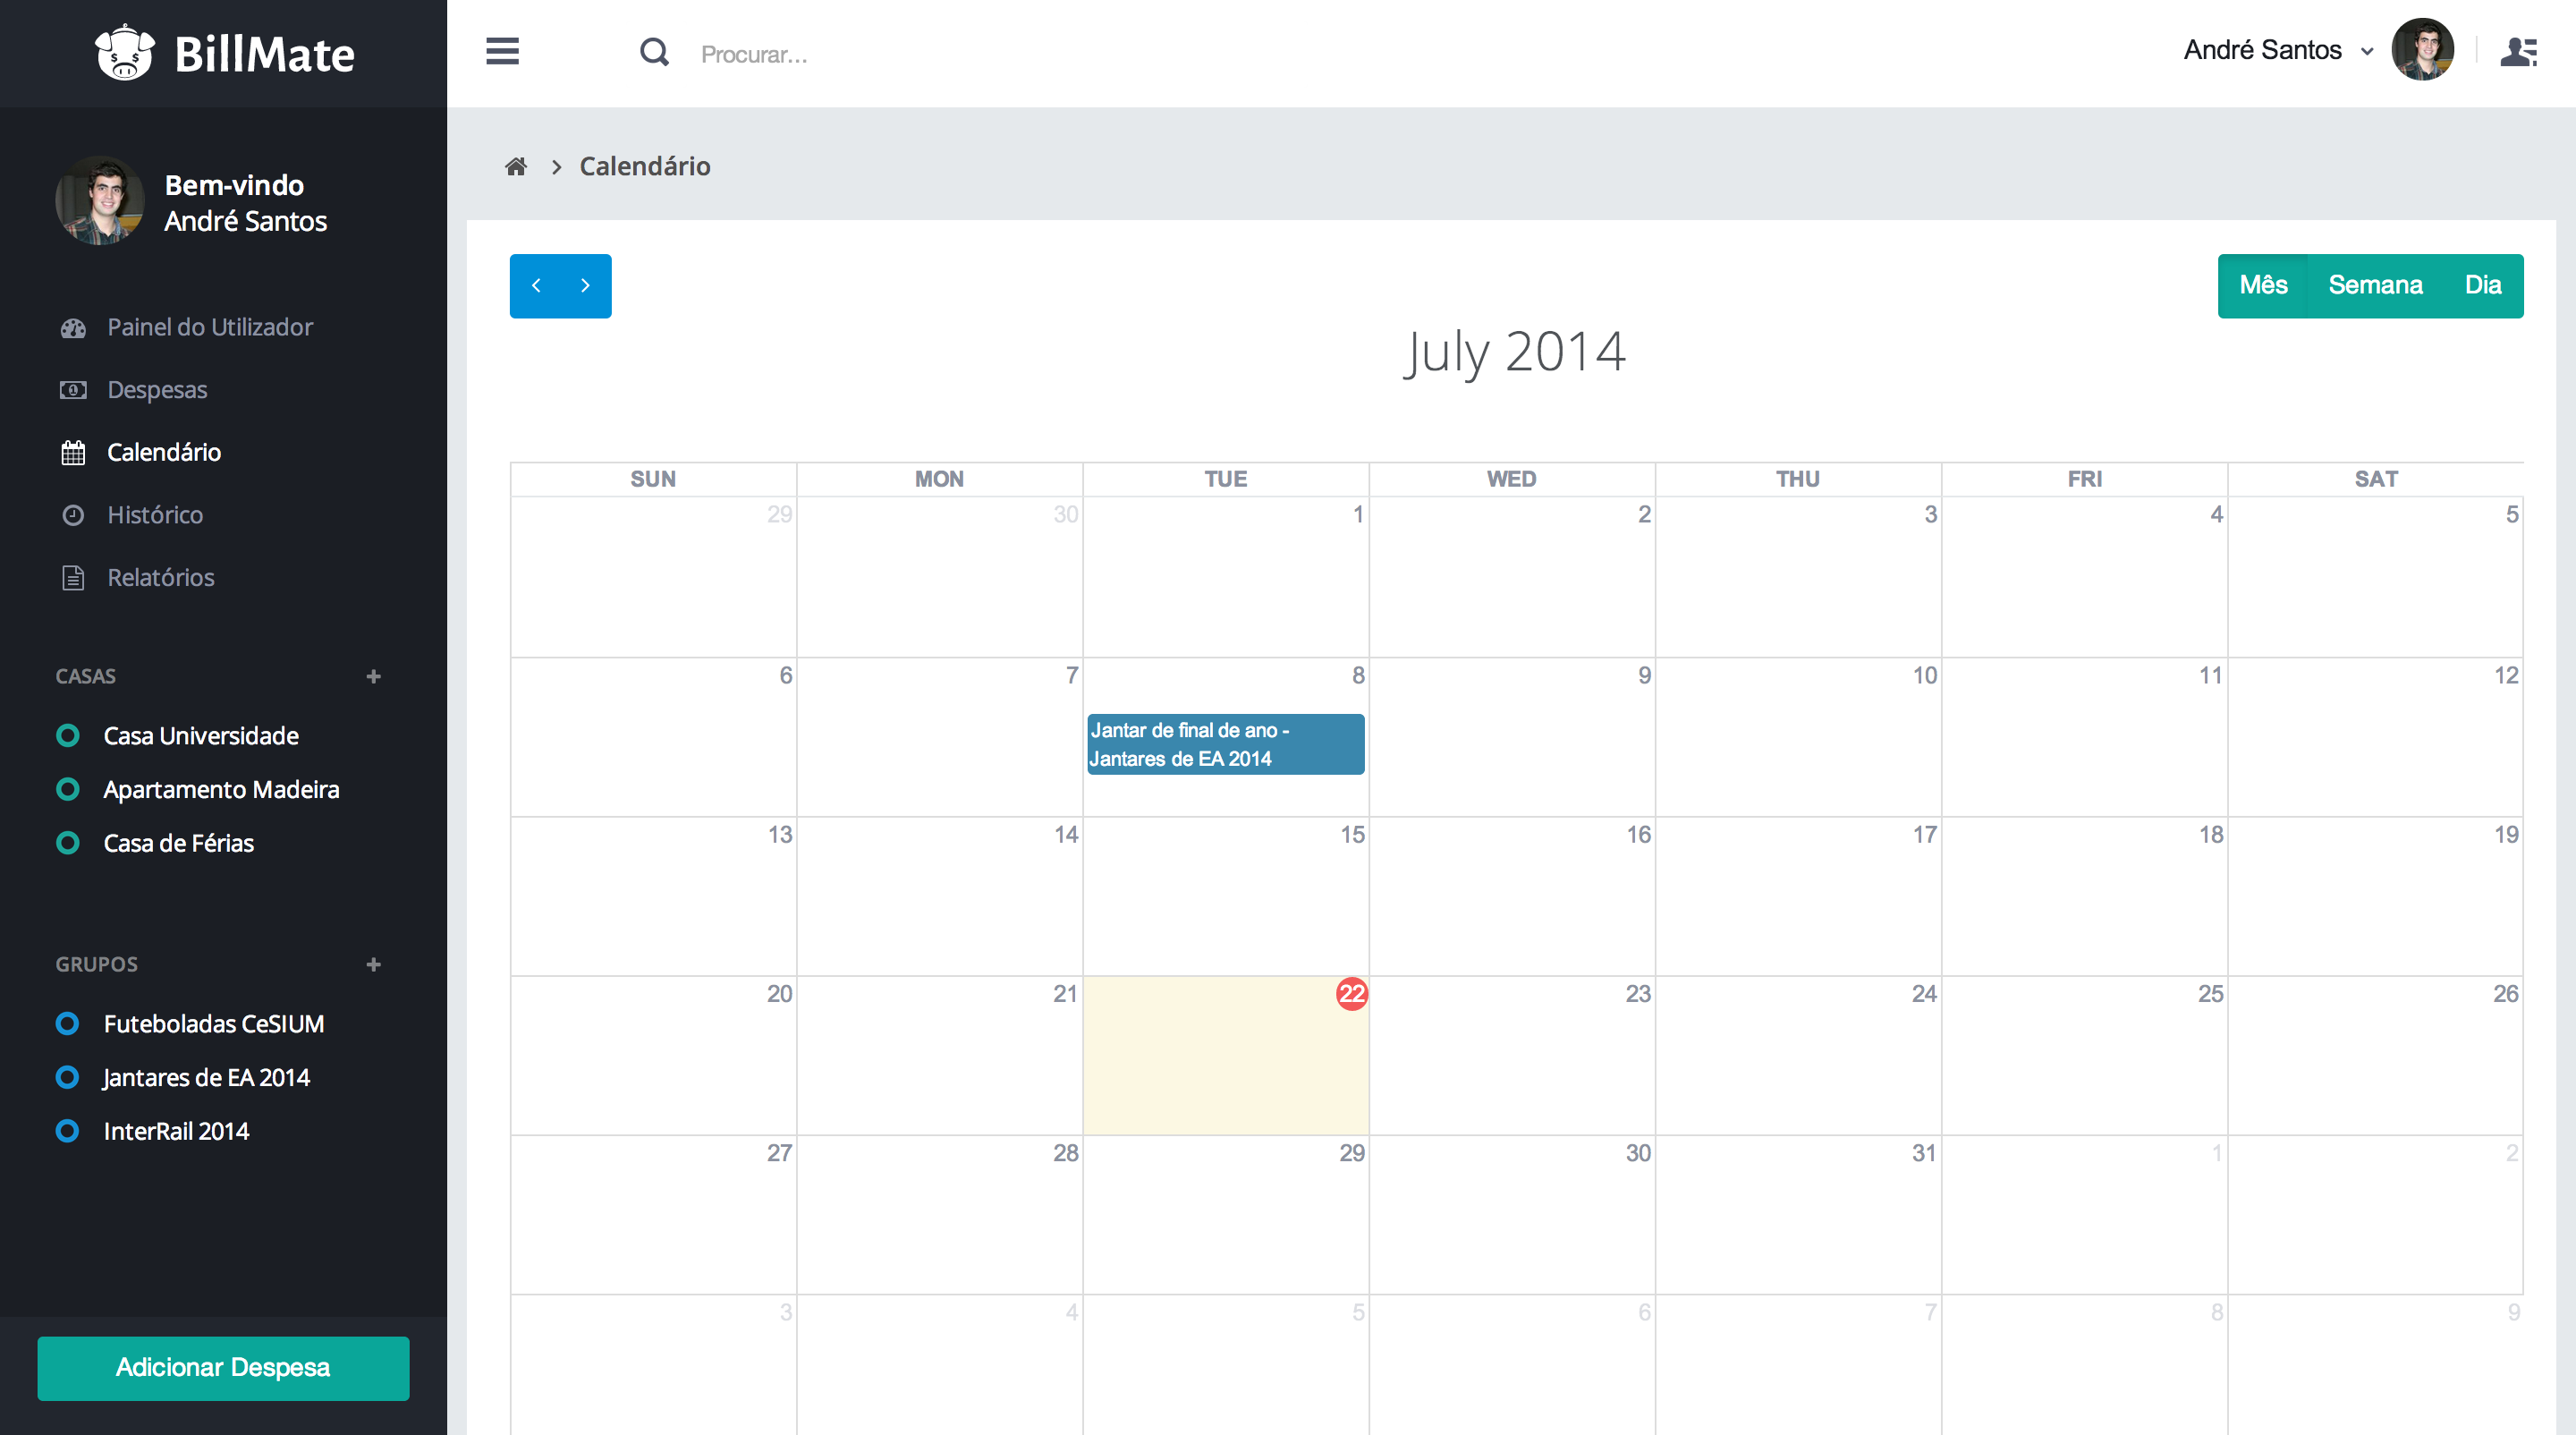
\includegraphics[width=.5\textwidth]{images/andre/calendar}
\caption{Calendário}
\end{figure}

\begin{figure}[ht]
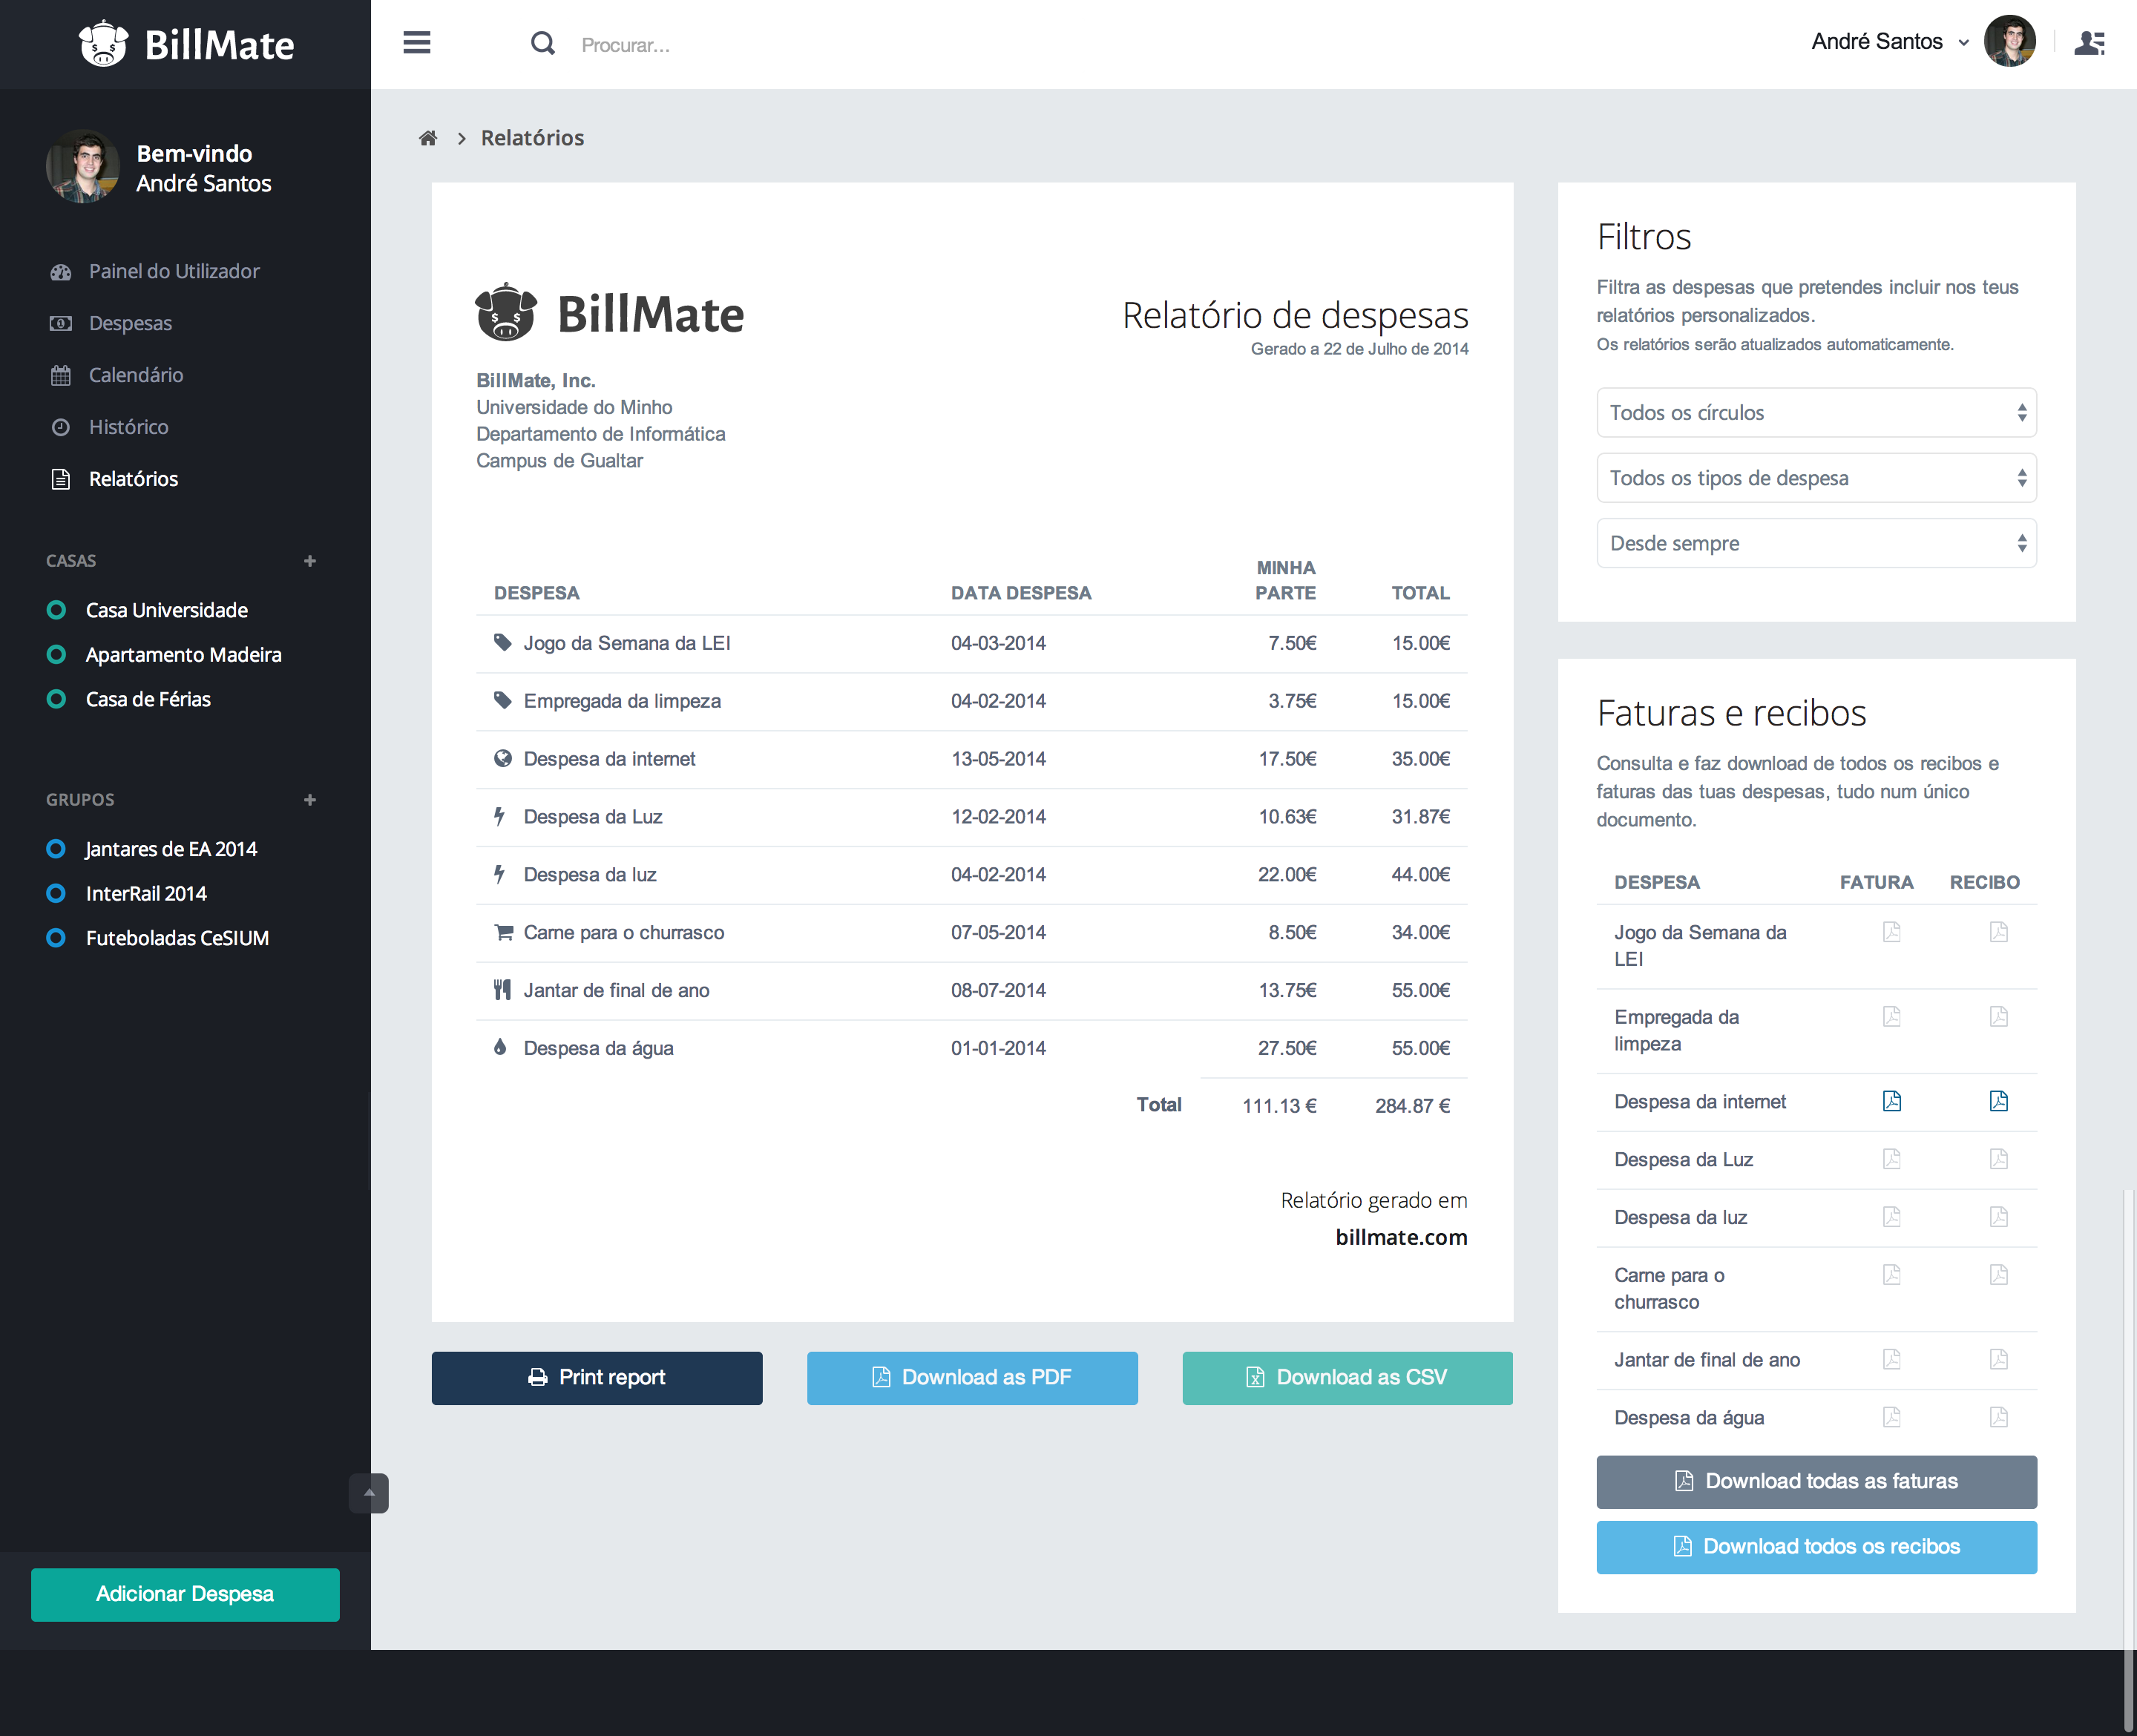
\includegraphics[width=.5\textwidth]{images/andre/reports}
\caption{Relatório}
\end{figure}

\end{referenciaswww}


%\chapter[How to?]
{Howto}

\section{Equações}

\begin{equation}
ABC {\cal DEF} \alpha\beta\Gamma\Delta\sum^{abc}_{def}
\end{equation}


\section{Referenciar a bibliografia}

zhamming - \cite{hamming} e ainda zHu - \cite{zHu}

\section{Inserir Imagem}

\begin{figure}[H]
\centerline{
\includegraphics[width=.5\textwidth]{images/dium}}
\caption{Legenda.}
\end{figure}

\pagebreak

Aqui está outra, mas inseri uma quebra de página para se conseguir separar as duas:

\begin{figure}[H]
\vskip2pt
\centerline{
\includegraphics[width=.5\textwidth]{images/dium}}
\caption{Oscillograph for  memory address access operations,
showing 500 ps
address access time and superimposed signals
of address access in 1 kbit
memory plane.}
\end{figure}


\pagebreak

\section{Inserir Tabela}

\begin{table}[ht]
\caption{Small Table}
\centering
\begin{tabular}{cccc}
\hline
one&two&three&four\\
\hline
C&D&E&F\\
\hline
\end{tabular}
\end{table}


\section{Inserir um Exemplo}
\vskip6pt
\begin{example}[Titulo do Exemplo]
Apresentar um exemplo de qualquer coisa.
\end{example}


\section{2 imagens lado a lado}

\begin{figure}[H]
\sidebyside{

\includegraphics[width=.5\textwidth]{images/dium}
\caption{Imagem da Esquerda}
}
{

\includegraphics[width=.5\textwidth]{images/dium}
\caption{Imagem da Direita}
}
\end{figure}


\section{Inserir Tabela de outro estilo}

\begin{table}[ht]
\caption{Effects of the two types of $\alpha\beta\sum^A_B$ scaling proposed by Dennard \newline
and
co-workers$^{a,b}$}
\begin{tabular*}{\textwidth}{@{\extracolsep{\fill}}lcc}
\hline
Parameter& $\kappa$ Scaling & $\kappa$, $\lambda$ Scaling\cr
\hline
Dimension&$\kappa^{-1}$&$\lambda^{-1}$\cr
Voltage&$\kappa^{-1}$&$\kappa^{-1}$\cr
Currant&$\kappa^{-1}$&$\lambda/\kappa^{2}$\cr
Dopant Concentration&$\kappa$&$\lambda^2/\kappa$\cr
\hline
\end{tabular*}
\begin{tablenotes}
$^a$Refs.~19 and 20.

$^b\kappa, \lambda>1$.
\end{tablenotes}
\end{table}


\section{Inserir Tabela lado a lado}

Tabelas lado a lado

 \begin{table}[ht]
 \sidebyside{
\caption{Table Caption}
\begin{tabular}{cccc}
one&two&three&four\\
a &little&sample&table
\end{tabular}
}
 {
\caption{Table Caption}
\begin{tabular}{cccc}
A&B&C&D\\
a &second little& sample&table
\end{tabular}
}
 \end{table}


\section{Usar Verbatim}

\begin{verbatim}
 \begin{table}
 \sidebyside{\caption{Table Caption}\label{tab1}
 first table}
 {\caption{Table Caption}\label{tab2} second table}
 \end{table}
\end{verbatim}



\section{Colocar Snippets}

\insertcode{snippets/example.pl}{Nena would be proud.}


\section{Colocar Algoritmo}

\begin{algorithm}
{\bf state\_transition algorithm} $\{$
\        for each neuron $j\in\{0,1,\ldots,M-1\}$
\        $\{$
\            calculate the weighted sum $S_j$ using Eq. (6);
\            if ($S_j>t_j$)
\                    $\{$turn ON neuron; $Y_1=+1\}$
\            else if ($S_j<t_j$)
\                    $\{$turn OFF neuron; $Y_1=-1\}$
\            else
\                    $\{$no change in neuron state; $y_j$ remains %
unchanged;$\}$
\        $\}$
$\}$
\end{algorithm}

\section{Inserir Citação}

\begin{quote}
	This is a sample of extract or quotation.
\end{quote}


\section{Criar Listas}

Tipo 1 \newline\newline

\begin{enumerate}
\item
This is the first item in the numbered list.

\item
This is the second item in the numbered list.
This is the second item in the numbered list.
This is the second item in the numbered list.
\end{enumerate}

Tipo 2 \newline\newline

\begin{itemize}
\item
This is the first item in the itemized list.

\item
This is the first item in the itemized list.
This is the first item in the itemized list.
This is the first item in the itemized list.
\end{itemize}

Tipo 3 \newline\newline

\begin{itemize}
\item[]
This is the first item in the itemized list.

\item[]
This is the first item in the itemized list.
This is the first item in the itemized list.
This is the first item in the itemized list.
\end{itemize}


\section{Criar Problemas}

\begin{problems}
\prob
For Hooker's data, Problem 1.2, use the Box and Cox and Atkinson procedures to determine a appropriate transformation of PRES
in the regression of PRES on TEMP. find $\hat\lambda$, $\tilde\lambda$,
the score test, and the added variable plot for the score.
Summarize the results.

\prob
The following data were collected in a study of the effect of dissolved sulfur
on the surface tension of liquid copper (Baes and Killogg, 1953).

{\centering
\vskip6pt
\begin{tabular}{rlcc}
\hline
&&\multicolumn2c{$Y$= Decrease in Surface Tension}\\
\multicolumn2c{$x$ = Weight \% sulfur}
&\multicolumn2c{(dynes/cm), two Replicates}\\
\hline
0.&034&301&316\\
0.&093&430&422\\
0.&30&593&586\\
\hline
\end{tabular}
\vskip6pt
}


\subprob
Find the transformations of $X$ and $Y$ sot that in the transformed scale
the regression is linear.

\subprob
Assuming that $X$ is transformed to $\ln(X)$, which choice of $Y$ gives
better results,
$Y$ or $\ln(Y)$? (Sclove, 1972).

\sidebysidesubprob{In the case of $\alpha_1$?}{In the case of $\alpha_2$?}

\prob
Examine the Longley data, Problem 3.3, for applicability of assumptions of the
linear model.

\sidebysideprob{In the case of $\Gamma_1$?}{In the case of $\Gamma_2$?}

\end{problems}


\section{Criar Exercícios}


\begin{exercises}
\exer
For Hooker's data, Exercise 1.2, use the Box and Cox and Atkinson procedures to determine a appropriate transformation of PRES
in the regression of PRES on TEMP. find $\hat\lambda$, $\tilde\lambda$,
the score test, and the added variable plot for the score.
Summarize the results.

\exer
The following data were collected in a study of the effect of dissolved sulfur
on the surface tension of liquid copper (Baes and Killogg, 1953).

{\centering
\vskip6pt
\begin{tabular}{rlcc}
\hline
&&\multicolumn2c{$Y$= Decrease in Surface Tension}\\
\multicolumn2c{$x$ = Weight \% sulfur}
&\multicolumn2c{(dynes/cm), two Replicates}\\
\hline
0.&034&301&316\\
0.&093&430&422\\
0.&30&593&586\\
\hline
\end{tabular}
\vskip6pt
}


\subexer
Find the transformations of $X$ and $Y$ sot that in the transformed scale
the regression is linear.

\subexer
Assuming that $X$ is transformed to $\ln(X)$, which choice of $Y$ gives
better results,
$Y$ or $\ln(Y)$? (Sclove, 1972).

\sidebysidesubexer{In the case of $\Delta_1$?}{In the case of $\Delta_2$?}

\exer
Examine the Longley data, Problem 3.3, for applicability of assumptions of the
linear model.

\sidebysideexer{In the case of $\Gamma_1$?}{In the case of $\Gamma_2$?}

\end{exercises}


\section{Criar Apêndice com o título}

\chapappendix{Titulo do Apêndice}
Aqui mete-se a descrição. Nota: O NOME DA LABEL FICA DIFERENTE, REALÇANDO QUE É UM APÊNDICE. EXEMPLO: FICA FIGURA 4-A.1
\begin{equation}
\alpha\beta\Gamma\Delta
\end{equation}


\begin{figure}[H]
\caption{This is an appendix figure caption.}
\end{figure}

\begin{table}[ht]
\caption{This is an appendix table caption}
\centering
\let\hline\savehline
\begin{tabular}{@{\vrule height 11pt depth 4pt width0pt}|l|p{.65\textwidth}|c}
\hline
{\bf Date} & \multicolumn1{c|}{\bf Event} \\
\hline \hline
1867 & Maxwell speculated the existence of electromagnetic waves.\\
1887 & Hertz showed the existence of electromagnetic waves. \\
1890 & Branly developed technique for detecting radio waves. \\
1896 & Marconi demonstrated wireless telegraph. \\
1897 & Marconi patented wireless telegraph.  \\
1898 & Marconi awarded patent for tuned communication. \\
1898 & Wireless telegraphic connection between England and France established. \\
\hline
\end{tabular}
\end{table}



\section{Criar Índice Remissivo}

pedro leite \index{pedro leite}.
andre santos \index{andre santos}.
francisco neves \index{francisco neves}.
ricardo branco \index{ricardo branco}.
Universidade do Minho \index{Universidade do Minho}.
Departamento de Informática \index{Universidade do Minho!Departamento de Informática}.
Departamento de Produção e Sistemas \index{Universidade do Minho!Departamento de Produção e Sistemas}.
Engenharia Informática \index{Departamento de Informática!Engenharia Informática}.


\begin{verbatim}
	pedro leite \index{pedro leite}.
	andre santos \index{andre santos}.
	francisco neves \index{francisco neves}.
	ricardo branco \index{ricardo branco}.
	Universidade do Minho \index{Universidade do Minho}.
	Departamento de Informática \index{Universidade do Minho!Departamento de Informática}.
	Departamento de Produção e Sistemas \index{Universidade do Minho!Departamento de Produção e Sistemas}.
	Engenharia Informática \index{Departamento de Informática!Engenharia Informática}.
\end{verbatim}



\printindex
\end{document}

